\documentclass[12pt]{article}
\usepackage{setspace}
\usepackage[margin=1in]{geometry}
\usepackage{graphicx}
\usepackage{amsmath}
\usepackage{amssymb}
\usepackage{amsthm}
\usepackage{amsbsy}
\newtheorem{proposition}{Proposition}
\newtheorem{aproposition}{Proposition}
\renewcommand{\theaproposition}{A.\arabic{theaproposition}}
\newtheorem{corollary}{Corollary}
\newtheorem{lemma}{Lemma}
\renewcommand{\theequation}{A.\arabic{theequation}}
\renewcommand{\theequation}{A.\arabic{equation}}
\newtheorem{assumption}{Assumption}
\usepackage{bbm}
\usepackage{varwidth}
\usepackage{enumitem}
\usepackage{float}
\usepackage[bottom]{footmisc}
\usepackage{natbib} %longnamesfirst
\bibpunct{(}{)}{;}{a}{}{,} % remove comma between author and year (fifth argument)

\usepackage[colorlinks=true, allcolors=blue]{hyperref}

\usepackage{scrextend}

\usepackage{array}
\usepackage{multirow}
\usepackage{float}

\usepackage{pdflscape}
\usepackage{comment}

\usepackage{indentfirst}

\usepackage{longtable}
\usepackage{pdfpages}

\usepackage{booktabs}

\renewcommand\thefigure{\thesection.\arabic{figure}}
\renewcommand\thetable{\thesection.\arabic{table}}

\title{\vspace*{2em} Appendix: Democracy in America? \\ Partisanship, Polarization, and the Robustness of Support for Democracy in the United States}
\author{Matthew H. Graham\thanks{Ph.D. Candidate, Department of Political Science, Yale University, \href{email:matthew.graham@yale.edu}{matthew.graham@yale.edu}.} \hspace{1mm} and Milan W. Svolik\thanks{Professor, Department of Political Science, Yale University, \href{email:milan.svolik@yale.edu}{milan.svolik@yale.edu}.}}
\date{First draft: March 2018, current version: December 2019}


\begin{document}

\maketitle

\newpage

\tableofcontents

\normalsize

\newpage
%\restoregeometry
\appendix
\onehalfspacing


\section{The Model}


Here we give formal statements, proofs, and illustrations of the theoretical results presented in the section ``A Model of the Public as a Democratic Check.’’ We first consider predictions 1-4 about $\Delta \downarrow$, then build on those results to support prediction 5.

The following proposition summarizes our analysis in the paper of the deterministic case with a single policy position $k$:
\begin{proposition} \label{prop: case1}
Let candidate~1's platform be to the right of candidate~2's platform, $x_{1k} > x_{2k}$. Then the fraction of voters who always vote for the more democratic of the two candidates is
\begin{equation*}
\Delta = F(x_{s}^1)- F(x_{s}^2),
\end{equation*}
where $F(x_{ik})$ is the distribution of voters' ideal points and $x_{s}^1, x_{s}^2$ are the swing voters
\begin{eqnarray*}
x_{s}^1 &=& \frac{x_{1k} + x_{2k}}{2} + \frac{\delta}{2 \alpha_k (x_{1k} - x_{2k})} \, , \\
x_{s}^2 &=& \frac{x_{1k} + x_{2k}}{2} - \frac{\delta}{2 \alpha_k (x_{1k} - x_{2k})} \, .
\end{eqnarray*}
\renewcommand{\labelenumi}{(\roman{enumi})}
\begin{enumerate}
\item $\Delta$ is increasing in support for democracy $\delta$;
\item $\Delta$ is decreasing in the intensity of voters' policy preferences $\alpha_k$;
\item $\Delta$ is decreasing in the distance between candidate platforms $x_{1k} - x_{2k}$;
\item $\Delta$ is decreasing in the degree to which the distribution of voters' ideal points is U-shaped, defined here the fraction of ideal points located below and above two values symmetric around the median $m$ of $F$, i.e. the sum $F(m-a) + [1-F(m+a)]$, where $0<a<|m|$.
\end{enumerate}
\end{proposition}

\begin{proof}
Parts (i)-(iii) are straightforward comparative statics on expressions for the swing voters $x_{s}^1$ and $x_{s}^2$ with respect to $\delta$, $\alpha$, and $x_{1k} - x_{2k}$.

To see part (iv), observe that, by our definition, the distribution $F(x_{ik})$ is more U-shaped than the distribution $G(x_{ik})$ if
\begin{equation*}
F(m-a) + [1-F(m+a)] > G(m-a) + [1-G(m+a)] \quad \text{for any} \quad 0<a<|m| \, .
\end{equation*}
In turn, a more U-shaped distribution will have a smaller fraction of voters located on the interval $(x_{s}^2, x_{s}^1)$, resulting in a smaller fraction $\Delta$ of voters who always vote for the more democratic of the two candidates.
\end{proof}

The following proposition summarizes our analysis in the paper of the stochastic case with a single policy position $k$:
\begin{proposition} \label{prop: case1}
Let candidate~1's platform be to the right of candidate~2's platform, $x_{1k} > x_{2k}$. Then the fraction of voters who defect from the candidate~1 when he adopts undemocratic position $M_1$ is
\begin{equation*}
\Delta = \int_{-\infty}^{\infty} \left(\frac{1}{1+e^{-\alpha_k D}}-\frac{1}{1+e^{-(\alpha_k D - \delta M_1)}}\right) dF(x_i),
\end{equation*}
where $F(x_i)$ is the distribution of voters' ideal points, $\frac{1}{1+e^{-X}}$ is the logistic function in $X$, and $D= (x_{ik} - x_{2k})^2 - (x_{ik} - x_{1k})^2$ is the difference in voter's policy payoff between the two candidate's platforms (in favor of candidate~1.)

\renewcommand{\labelenumi}{(\roman{enumi})}
\begin{enumerate}
\item $\Delta$ is increasing in support for democracy $\delta$,
\item $\Delta$ is decreasing in the intensity of voters' policy preferences $\alpha_k$,
\item $\Delta$ is decreasing in the distance between candidate platforms $x_{1k} - x_{2k}$,
\item $\Delta$ is decreasing in the degree to which the distribution of voters' ideal points is U-shaped, defined here by the sum $F(m-a) + [1-F(m+a)]$, where $0<a<|m|$ (the fraction of ideal points located below and above two values symmetric around the median $m$ of $F$.)
\end{enumerate}
\end{proposition}

\begin{proof}
Assuming that the error terms $\epsilon_{ij}$ are (independently) drawn from type I extreme value distribution (also known as the standard Gumbel distribution) implies that voter $i$'s probability of voting for candidate~1 is shaped by the difference in voter $i$'s payoff from the two candidates according to the logistic function,\footnote{For an explicit derivation of how type I extreme value distributed error terms imply the logistic model, see e.g. \citet[476-478, 486-487]{Cameron2005}.}
\begin{equation*}
\text{Pr}(i \text{ votes for candidate~1}) = \frac{1}{1+e^{-[u_i(X_1, M_1)-u_i(X_2, M_2)]}} \, .
\end{equation*}
The difference in voter $i$'s payoff from the two candidates $u_i(X_1, M_1)-u_i(X_2, M_2)$ then becomes $\alpha_k D$ when $M_1=M_2=0$ and $\alpha_k D - \delta M_1$ when $M_1=1$ and $M_2=0$.

Parts (i)-(iii) are straightforward comparative statics on the $\frac{1}{1+e^{-\alpha_k D}}-\frac{1}{1+e^{-(\alpha_k D - \delta M_1)}}$ part of $\Delta$ with respect to $\delta$, $\alpha$, and $x_{1k} - x_{2k}$.

To see part (iv), observe that the difference $\frac{1}{1+e^{-\alpha_k D}}-\frac{1}{1+e^{-(\alpha_k D - \delta M_1)}}$ has a unique global maximum at the ideal point
\begin{equation*}
x^1_{\Delta} = \frac{x_{1k} + x_{2k}}{2} + \frac{\delta}{4 \alpha_k (x_{1k} - x_{2k})} \, ,
\end{equation*}
and is strictly increasing for any $x_{ik}<x^1_{\Delta}$ and strictly decreasing for any $x_{ik}>x^1_{\Delta}$. Furthermore,
\begin{equation*}
\frac{x_{1k} + x_{2k}}{2} < x^1_{\Delta} < x_{s}^1 \, ,
\end{equation*}
that is, voter $x^1_{\Delta}$ is to the right of the median but to the left of the swing voter $x_{s}^1$. By the same argument, when $M_1=0$ and $M_2=1$, the difference $-(\frac{1}{1+e^{-\alpha_k D}}-\frac{1}{1+e^{-(\alpha_k D + \delta M_2)}})$ has the unique global maximum
\begin{equation*}
x^2_{\Delta} = \frac{x_{1k} + x_{2k}}{2} - \frac{\delta}{4 \alpha_k (x_{1k} - x_{2k})} \, ,
\end{equation*}
and is strictly increasing for any $x_{ik}<x^2_{\Delta}$ and strictly decreasing for any $x_{ik}>x^2_{\Delta}$. Furthermore,
\begin{equation*}
x_{s}^2 < x^2_{\Delta} < \frac{x_{1k} + x_{2k}}{2} \, .
\end{equation*}
This implies that voters with ideal points on the interval $(x_{s}^2, x_{s}^1)$ vote for the more democratic of the two candidates with a probability greater than one-half, regardless of which of the two candidates adopts an undemocratic platform. (By our definition of a swing voter, swing voter $x_{s}^1$ votes for candidate~1 with the probability one-half when $M_1=1$ and $M_2=0$; swing voter $x_{s}^2$ votes for candidate~2 with the probability one-half when $M_1=0$ and $M_2=1$.) Voters outside the interval $(x_{s}^2, x_{s}^1)$ vote for the \emph{less} democratic candidate when that candidate is closer to them policy-wise with a probability greater than one-half. 
By our definition, the distribution $F(x_{ik})$ is more U-shaped than the distribution $G(x_{ik})$ if
\begin{equation*}
F(m-a) + [1-F(m+a)] > G(m-a) + [1-G(m+a)] \quad \text{for any} \quad 0<a<|m| \, .
\end{equation*}
In turn, a more U-shaped distribution will have a smaller fraction of voters located on the interval $(x_{s}^2, x_{s}^1)$, resulting in a smaller fraction voters who always vote for the more democratic of the two candidates with a probability greater than one-half and a greater fraction voters who for the less democratic candidate when that candidate is closer to them policy-wise.
\end{proof}

Figure \ref{fig: beta} illustrates part (iv) of Proposition 2 by plotting the fraction of voters who defect from an undemocratic candidate as the distribution of voters becomes more U-shaped. We do this by drawing voters' ideal policies from the symmetrical $Beta(\gamma, \gamma)$ density. The left panel shows that a decrease in the parameter $\gamma$ from 5 to $\frac{1}{5}$ corresponds to the shift from a centrist distribution of voter ideal points to one that is U-shaped.\footnote{The remaining parameter values are $\alpha_k= 8$, $\delta= 2$, $x_{1k}= 1/5$, $x_{2k}= -1/5$, $M_1=1$, which implies $x_{s}^1=-x_{s}^2=5/16$.} The right panel plots the resulting decrease in the fraction of voters who defect from candidate~1 when he adopts undemocratic position $M_1$.

\begin{figure}[t]
\centering
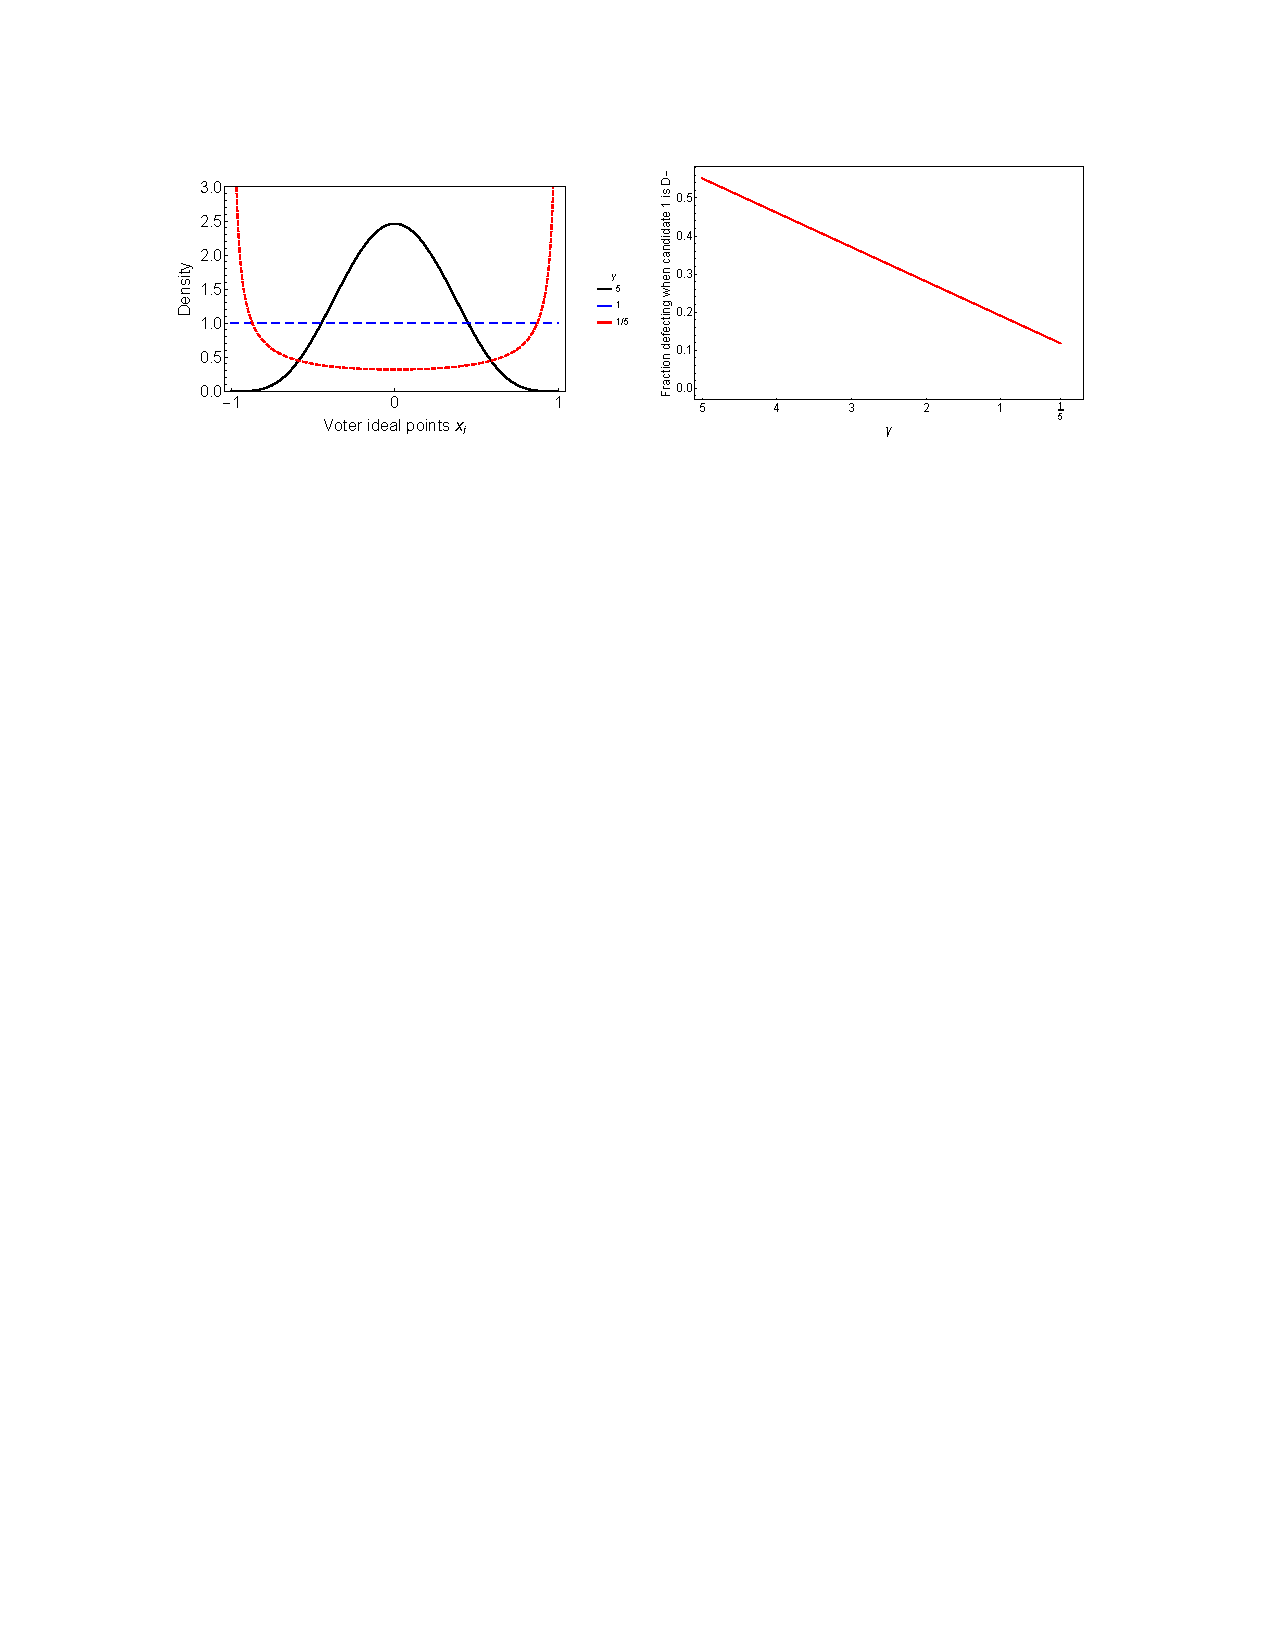
\includegraphics{figures/appendix_model_beta.pdf}
\caption{$Beta(\gamma, \gamma)$ distribution of voters' ideal points (left) and the decline in the less democratic candidate's vote share (right) associated the shift from a centrist distribution of voter ideal points ($\gamma=5$) to a U-shaped one ($\gamma=1/5$) }
\label{fig: beta}
\end{figure}

The proof of part (iv) of Proposition 2 contains two corollaries that we evaluate using data from our candidate-choice experiment. We therefore state them explicitly below: 
\begin{corollary} 
The segment between the two swing voters, $(x_{s}^2, x_{s}^1)$, delineates voters who in the treatment condition $D^- \text{ vs. } D^+$ vote for the $D^+$ candidate with a probability greater than one-half, regardless of which of the two candidates is closer to them policy-wise,
\begin{equation*}
\text{Pr}(i \text{ votes for the $D^+$ candidate } | D^- \text{ vs. } D^+ ) > \frac{1}{2} \quad \text{for all} \quad x_{ik} \in (x_{s}^2, x_{s}^1).
\end{equation*}
\end{corollary}
This segment of voters is shown in the left panel of Figure 1 in the main text.

\begin{corollary} 
Denote the ideal point of voters who in the treatment condition $D^- \text{ vs. } D^+$ defect from the $D^-$ candidate at the highest rate by $x^1_{\Delta}$, 
\begin{equation*}
x^1_{\Delta} = \frac{x_{1k} + x_{2k}}{2} + \frac{\delta}{4 \alpha_k (x_{1k} - x_{2k})} \, .
\end{equation*}
Voters with the ideal point $x^1_{\Delta}$ are located to the right of the median $\frac{x_{1k} + x_{2k}}{2}$ but to the left of the swing voter $x_{s}^1$, 
\begin{equation*}
\frac{x_{1k} + x_{2k}}{2} < x^1_{\Delta} < x_{s}^1 \, .
\end{equation*}
\end{corollary}
The right panel in Figure 1 in the main text illustrates Corollary 2.

Both propositions generalize to the case with $K$ policy positions after accounting for the fact that voter ideal points are now distributed according to a multivariate joint distribution $F(x_{i1}, \dots, x_{iK})$, which implies that we need to extend our definition of the degree to which a distribution is U-shaped to the multivariate context. We will say that the distribution $F(x_{i1}, \dots, x_{iK})$ is more U-shaped than the distribution $G(x_{i1}, \dots, x_{iK})$ if
\begin{multline*}
F(\dots, m-a, \dots) + [1-F(\dots, m+a, \dots)] > G(\dots, m-a, \dots) + [1-G(\dots, m+a, \dots)] \\
\text{for all } k \in K \text{ and for any } 0<a<|m| \, .
\end{multline*}

When $K \ge 2$, swing voters $x_{s}^1$ and $x_{s}^2$ are no longer characterized by unique ideal policy points but by hyperplanes satisfying the indifference conditions
\begin{equation*}
u_i(X_1, M_1=1) = u_i(X_2, M_2=0) \quad \text{and} \quad u_i(X_1, M_1=0) = u_i(X_2, M_2=1) \, .
\end{equation*}

\begin{figure}[t]
\centering
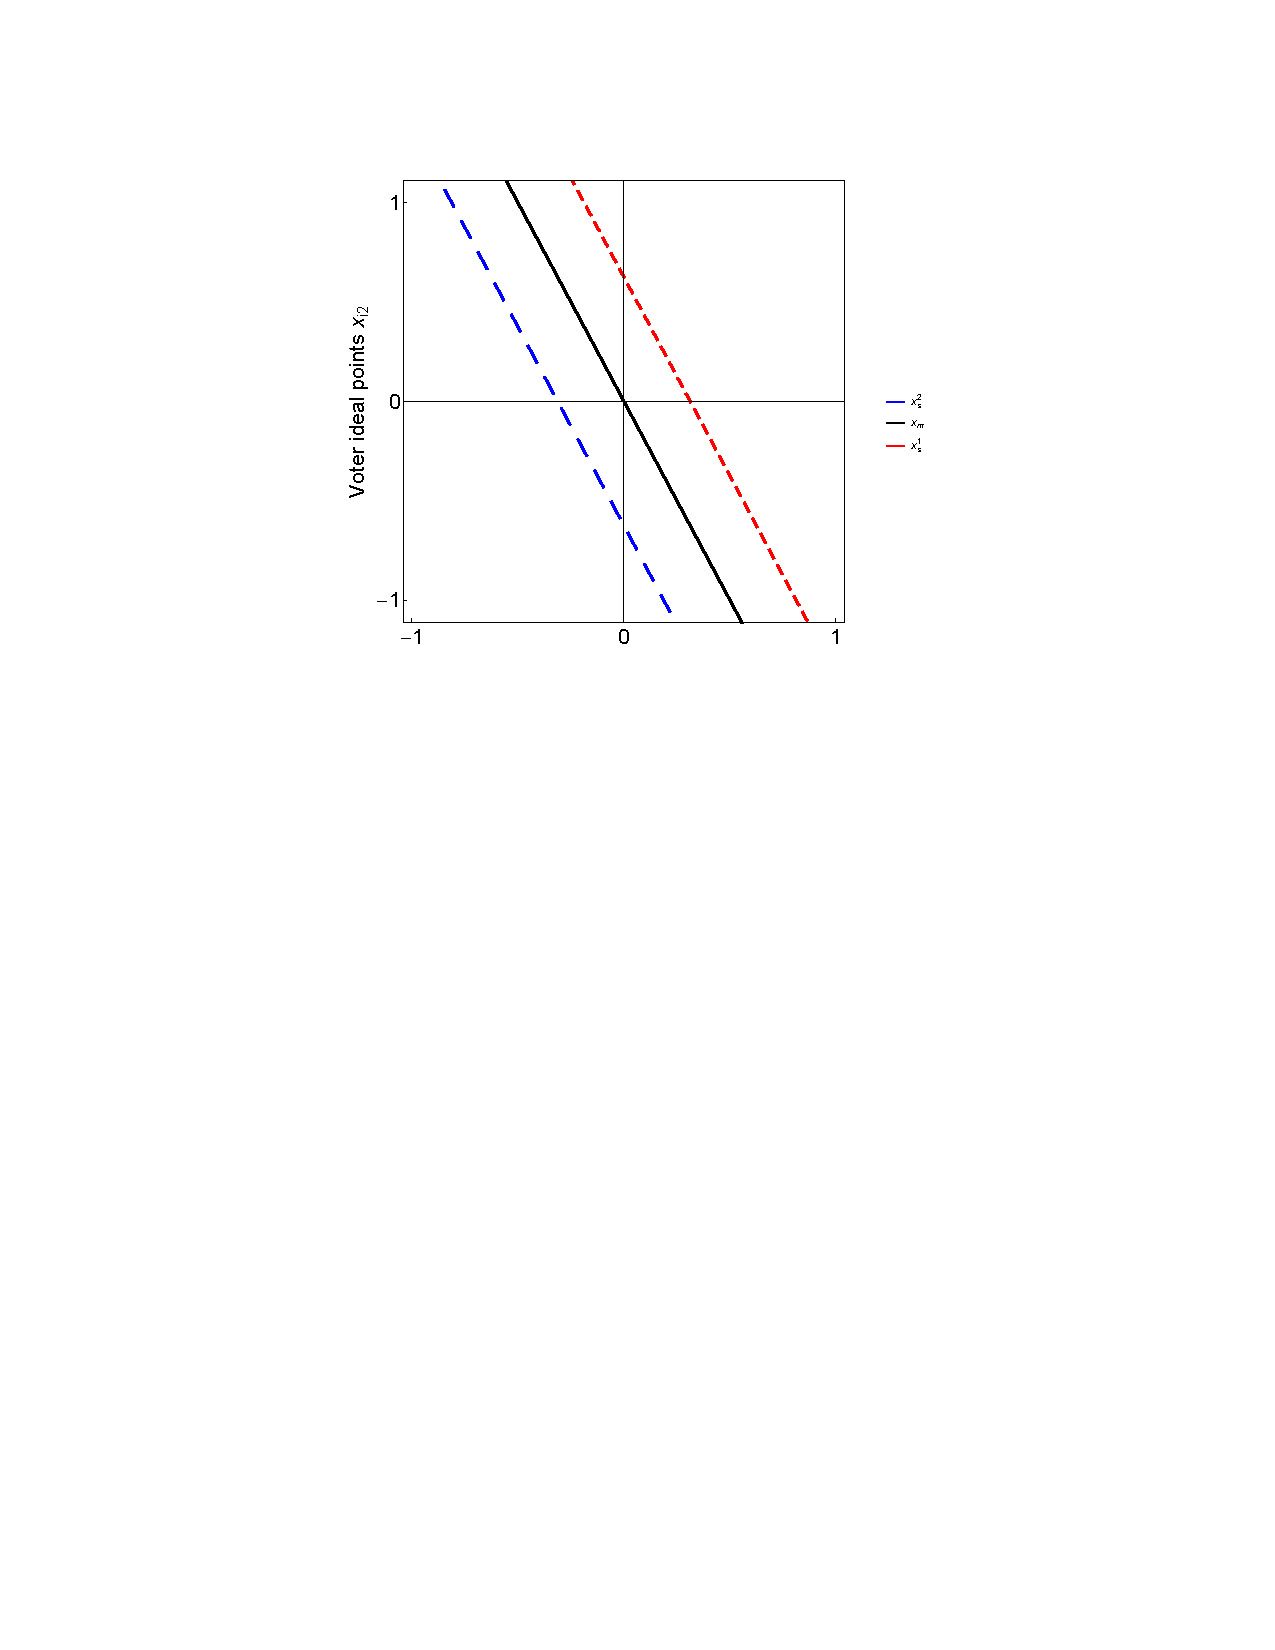
\includegraphics{figures/appendix_model_2k.pdf}
\caption{An illustration of the two-issue case, $K=2$}
\label{fig: k2}
\end{figure}

Figure \ref{fig: k2} illustrates swing voters $x_{s}^1$ and $x_{s}^2$ for the two-issue case, $K=2$, and parameter values $\alpha_1= 8$, $\alpha_1= 4$, $\delta= 2$, $x_{11}=x_{12}=1/5$, $x_{21}= x_{22}= -1/5$, $M_1=M_2=1$. This results in swing voters $x_{s}^1$ and $x_{s}^2$ that are characterized by the equations
\begin{equation*}
x_{i2} = \frac{5}{8} - 2 x_{i1} \quad \text{and} \quad x_{i2} = - \frac{5}{8} - 2 x_{i1} .
\end{equation*}
The solid black line in Figure \ref{fig: k2} plots voters who are indifferent between the two candidates when both adopt democratic positions, $M_1=M_2=0$ (i.e. the equivalent of the median voter in the single-issue case.) The red and blue dashed lines plot swing voters $x_{s}^1$ and $x_{s}^2$. Note that the slopes of these lines are steeper than $-1$, which is due to our assumption in this illustration that voters care twice as much about issue 1 as they care about issue 2.

A distinct prediction that arises only in the case of more than one issue concerns cross-cutting cleavages. Specifically, in the paper we anticipate that the fraction of voters who defect from a candidate that adopts an undemocratic position is smaller when voters' preferences over the $K$ distinct issues are aligned as opposed to cross-cutting with respect to candidates platforms. To see this, fix candidates' platforms and define a voter's policy preferences as \emph{aligned} if her ideal point $x_{ik}$ is closer to one candidate on all $K$ issues; otherwise, we say that the voter's policy preferences are \emph{cross-cutting}. This implies that the difference in a voter's overall policy distance from the two candidates, $\sum_{K} \alpha_k [(x_{ik} - x_{2k})^2 - (x_{ik} - x_{2k})^2]$, will be larger for voters whose policy preferences are aligned than for voters whose policy preferences are cross-cutting. This follows from our assumption that voters' policy preference over the $K$ issues are additive: for voters with cross-cutting preferences, a voter's greater distance from a candidate on one issue is at least partially cancelled out by her greater proximity to that candidate on another issue. In effect, voters with aligned policy preferences see an overall greater policy difference between candidates than do voters whose preferences are cross-cutting, parallelling part (iii) in Propositions 1 and 2.

%%%%%%%%%%%%%%%%%%%%%%%%%%%%%%%%%%%%%%%%%%%%%%%%%%%%%5
%%%%%%%%%%%%%%%%%%%%%%%%%%%%%%%%%%%%%%%%%%%%%%%%%%%%%%

\newpage

\section{Real-World Examples of Undemocratic Pcractices}
\setcounter{figure}{0} 
\setcounter{table}{0} 

An important criterion in the design of our treatments is that they be realistic and can be plausibly adopted by both major parties. Accordingly, the undemocratic positions our candidates take are situated at the state level, where most attempts to subvert the democratic process for partisan gain in the United States occur and have historically been attempted by both major parties.

In this section, we explain the design of each treatment in more detail and provide recent real-world examples of each treatment. We will see that treatments concerning both electoral manipulation and checks and balances reflect practices that are frequently threatened and often carried out (gerrymandering, voter suppression, executive orders, and threats to judicial independence.) Real-world violations of civil liberties rarely manifest as explicitly as they do in our treatments, but they do reflect positions that politicians openly express and occasionally act upon (banning protests, prosecuting journalists.)

\subsection{Electoral fairness}

Treatments capturing positions that aim to undermine the fairness of elections focused on two issues: i) gerrymandering, and ii) voter suppression.

\subsubsection*{i) Gerrymandering}

Gerrymandering -- the manipulation of electoral district boundaries for partisan gain -- is one of the oldest and best-known forms of electoral manipulation practiced in the United States \citep{McGannSmithLatnerEtAl2016,Seabrook2017}.\footnote{The term ``gerrymander" was coined in 1812 after Massachusetts Democratic-Republicans redrew district boundaries to disadvantage the rival Federalists. One particularly egregious district was shaped like a salamander. Though governor Elbridge Gerry is said to have been minimally involved in the process, the term ``gerrymander'' stuck.} Because state legislatures are in charge of drawing electoral districts in most states, parties that control the process often draw the boundaries to give their own party a disproportionate number of seats in the state legislature and the U.S. House of Representatives.\footnote{See \citet{MaglebyMcDonaldKrasnoEtAl2018} for a review.}

We designed our treatment to unambiguously communicate this type of manipulation without using a loaded term like gerrymandering. Accordingly, our candidates have

\begin{center}
\begin{varwidth}{\linewidth}
\begin{verbatim}
Supported a redistricting plan that gives [own party]s
[2 or 10] extra seats despite a decline in the polls.
\end{verbatim}
\end{varwidth}
\end{center}

While the identification of a workable standard for judging when a partisan bias in redistricting is extreme enough to be ``unfair'' is the subject of active research \citep{Chen2013,ChoLiu2016}, compelling evidence of recent partisan gerrymandering exists for a number of states, including Maryland, North Carolina, Ohio, Pennsylvania, Texas, and Wisconsin.\footnote{See e.g. Laura Royden, Michael Li, and Yurij Rudensky, ``Extreme Gerrymandering \& the 2018 Midterm,'' \emph{Brennan Center for Justice at New York University School of Law}.}

One example that captures our treatment's realism especially well occurred in 2011 in Maryland, where former Governor Martin O'Malley (D-MD) admitted to using his influence over the redistricting process to produce a map that favored Democrats. O'Malley said shifting a seat from a Republican to Democrat was ``certainly my hope, and it was part of my intent.''\footnote{Brian Witte, ``\href{https://www.heraldmailmedia.com/news/annapolis/o-malley-intended-redistricting-map-to-favor-md-democrats/article\_b368d498-797d-5c1a-9cba-7fb707ab737b.html}{O'Malley intended redistricting to favor Md. Democrats},'' \emph{Herald-Mail}, June 1, 2017.} Democrats undertook this effort in 2011 despite a decline in the House vote share from 67 percent to 60 percent between 2008 and 2010.\footnote{Dave Leip, ``\href{https://uselectionatlas.org/}{Atlas of U.S. Presidential Elections},'' accessed via Yale University Libraries.}

\subsubsection*{ii) Voter suppression}

Electoral manipulation and voter suppression have a long history in the United States \citep{Campbell2005,Bateman2018,Keyssar2000}. The Supreme Court's 2013 Shelby v. Holder decision to overturn the Voting Rights Act's requirement that states with a history of disenfranchisement pre-clear any changes to election procedures has coincided with a resurgence of voting restrictions at the state level (especially restrictions on early voting, same-day registration, and stricter voter ID requirements).\footnote{See \citet{BergmanTranYates2018} and ``Election 2016: Restrictive Voting Laws by the Numbers,'' \emph{Brennan Center for Justice at New York University School of Law}, September 28, 2016.} Before turning to our treatment, we present exemplars of some of the tactics currently in use.

\begin{itemize}
\item \textbf{Voter identification laws}: Between 2004 and 2016, the number of states with voter ID laws classified as ``strict'' by the National Conference of State Legislatures (NCSL) increased from zero to 11.\footnote{NCSL, ``\href{http://www.ncsl.org/research/elections-and-campaigns/voter-id-history.aspx}{History of Voter ID},'' May 31, 2017.} The majorities enacting these laws tend to favor forms of identity documents that their supporters disproportionately possess and disallow forms of ID that their opponents tend to use. In Pennsylvania, state House Republican leader Mike Turazi predicted that the state's voter ID law ``is gonna allow Governor Romney to win the state of Pennsylvania, done.''\footnote{MacKenzie Weigner, ``\href{https://www.politico.com/story/2012/06/pa-pol-voter-id-helps-gop-win-state-077811}{Pa. pol: Voter ID helps GOP win state},'' \emph{Politico}, June 25, 2012.} In Texas, Ansolabehere and Hersh (2017) found that S.B. 14, the voter ID law passed by Texas Republicans, disproportionately affected black and Hispanic voters; the law also disallowed the use of student IDs. The law was struck down in court due to its discriminatory intent.\footnote{Ariane de Vogue and Steve Almasy, ``\href{https://www.cnn.com/2017/08/23/politics/texas-voter-id-ruling/index.html}{New Texas voter ID law discriminates, federal judge rules},'' \emph{CNN}, August 23, 2017.}

\item \textbf{Restrictions on the time and location of voting}: State legislatures frequently attempt to change the available times and locations of voting to their political opponents' disadvantage. In particular, some Republican legislatures have restricted early and weekend voting options favored by low-income and black voters.\footnote{Steven Yaccino and Lizette Alvarez, ``\href{https://www.nytimes.com/2014/03/30/us/new-gop-bid-to-limit-voting-in-swing-states.html}{New G.O.P. Bid to Limit Voting in Swing States},'' \emph{The New York Times}, March 29, 2014.''} In Wisconsin, the Republican legislature passed a law, later struck down, that limited all cities to one early voting location.\footnote{Patrick Marley and Jason Stein, ``\href{https://www.jsonline.com/story/news/politics/2016/07/30/judge-strikes-down-wisconsin-voter-id-early-voting-laws/87803408/}{Judge strikes down Wisconsin voter ID, early voting laws},'' \emph{The Milwaukee Journal Sentinel}, July 30, 2016.} Almost immediately after the Supreme Court ruling in Shelby v. Holder, the North Carolina legislature used data on demographic voting patterns to devise a package of voting changes that the Fourth Circuit Court of Appeals later ruled had been designed to target black voters ``with almost surgical precision.''\footnote{\href{https://electionlawblog.org/wp-content/uploads/nc-4th.pdf}{North Carolina NAACP v. McCrory}, U.S. Court of Appeals for the Fourth Circuit, July 29, 2016.} The changes included shortening the early voting period, eliminating same-day registration, eliminating preregistration for young people, eliminating provisional ballots for people who went to the wrong precinct in the correct county, and changing registration requirements to eliminate forms of identification disproportionately used by black voters.

\item \textbf{Impeding voter registration}: The practice of ``voter caging,'' or sending a non-forwardable letter to geographic areas that tend to support opponents and challenging the registration of voters whose letter is returned to sender, has been a common practice in the United States since the 1950s.\footnote{Project Vote, ``\href{http://www.projectvote.org/wp-content/uploads/2010/02/2010-Legislative-Brief-Voter-Intimidation-and-Caging.pdf}{Voter Intimidation and Caging},'' February 2010.} The purpose of this tactic is to prevent or overturn the registration of voters who support the opposing party. Organized groups recruit volunteers to use century-old voter challenge laws to dispute the registration of eligible voters at the polls. These challenges are almost never upheld by courts, but they do appear to successfully intimidate voters.\footnote{Nicholas Riley, ``\href{http://www.brennancenter.org/sites/default/files/legacy/publications/Voter_Challengers.pdf}{Voter Challengers},'' \emph{The Brennan Center}, August 30, 2012.}

\item \textbf{Misinformation about procedures}: Robocalls, fliers, and billboards with false information about voting locations, times, and identity requirements are a common feature of American elections.\footnote{Common Cause, ``\href{https://www.commoncause.org/resource/deceptive-practices-2-0-legal-and-policy-responses/}{Deceptive Practices 2.0: Legal and Policy Responses},'' October 2008.} For example, although the Pennsylvania and Texas voter ID laws described above were each struck down in court, signage indicating that photo ID was required remained in place at some polling places.\footnote{Michaela Winberg, ``\href{https://billypenn.com/2018/05/07/no-you-dont-need-photo-id-to-vote-in-pennsylvania/}{Do you need photo ID to vote in PA? No, but there's good reason for confusion},'' \emph{Billy Penn}, May 7, 2018. Alex Samuels, ``\href{https://www.texastribune.org/2016/10/28/early-voting-issues-texas/}{Texas civil rights advocates air concerns about voter ID issues}, October 28, 2016.}

\item \textbf{Ballot fraud}: In 2018, the Republican Candidate in North Carolina's ninth U.S. House district, Mark Harris, hired a political consultant, Leslie McCrae Dowless, who along with several accomplices collected and filled in absentee ballots for the purpose of manipulating the outcome of the election. After months of resistance, Harris called for a new election following the presentation of overwhelming evidence that fraud occurred\footnote{Ely Portillo and Jim Morrill, ``\href{https://www.charlotteobserver.com/news/politics-government/article226550555.html}{Mark Harris calls for new election in 9th district},'' \emph{Charlotte Observer}, February 21, 2019.}---including testimony by Harris's son, John Harris, that he had warned his father about Dowless' illegal practices.\footnote{Laura Barron-Lopez, ``\href{https://www.politico.com/story/2019/02/20/mark-harris-north-carolina-election-fraud-1192738}{Mark Harris' son warned him about operative in North Carolina scandal},'' \emph{Politico}, February 20, 2019.} Dowless is under investigation for similar practices in the 2016 election.\footnote{Dan Kane and Ely Portillo, ``\href{https://www.newsobserver.com/news/politics-government/article222806255.html}{The `guru of Bladen County' is at the center of NC’s election troubles,'' \emph{News and Observer}, December 9, 2018.}} The publicity associated with these incidents is drawing attention to what may be a more longstanding pattern of manipulation in Bladen and Robeson counties.\footnote{Bruce Henderson and Will Doran, ``\href{https://www.newsobserver.com/news/politics-government/election/article222739860.html}{In 2 NC counties with `rough politics,' election fraud claims are nothing new},'' \emph{News and Observer}, January 26, 2019} Though we are not aware of similar recent events in other states, North Carolina's unusually transparent electoral data makes suspicious patterns easier to spot.\footnote{Nate Cohn, ``\href{https://www.nytimes.com/2018/12/07/upshot/mapped-why-voting-anomalies-are-impossible-to-ignore-in-north-carolina.html}{Why Voting Anomalies Are Impossible to Ignore in North Carolina},'' \emph{The New York Times}, December 7, 2018.}

\end{itemize}

For incumbent parties seeking to tilt the playing field in their favor, these types of changes are convenient because they can also occur for legitimate reasons. The voter identification requirements described above are often justified in terms of preventing voter fraud. Changing the location of polling places can be justified by shifts in population patterns, as was the case when 170 Democratic-leaning precincts were eliminated in Lake County, Indiana.\footnote{``\href{https://www.nwitimes.com/news/local/lake/update-secretary-of-state-trims-lake-county-s-precinct-map/article_3df5b288-c591-5b79-9014-4e94b137a3d5.html}{Secretary of state trims Lake County's precinct map by a third. Democrats cry foul.}’’ Northwest Indiana Times, August 1, 2018.} Cuts to the number of polling places can be necessitated by budget crisis\footnote{Matt Vasilogambros, ``\href{https://www.pewtrusts.org/en/research-and-analysis/blogs/stateline/2018/09/04/polling-places-remain-a-target-ahead-of-november-elections}{Polling Places Remain a Target Ahead of November Elections},’’ Pew Stateline, September 4, 2018.} or to a shift toward absentee voting.

For our candidate-choice experiment, we chose a treatment from the ``restrictions on the time and location of voting'' category. A candidate
\begin{center}
\begin{varwidth}{\linewidth}
\begin{verbatim}
Supported a proposal to reduce the number of polling stations
in areas that support [opposite party]s.
\end{verbatim}
\end{varwidth}
\end{center}

The closure of polling places has been an increasing national trend since the Shelby v. Holder decision: nationwide, the total number of polling stations dropped from 119,968 to 116,990 between 2012 and 2016.\footnote{Election Assistance Commission, ``\href{https://www.eac.gov/documents/2017/11/15/eavs-deep-dive-poll-workers-and-polling-places/}{EAVS Deep Dive},'' November 15, 2017.} Civil Rights organizations have cited a larger number of closures.\footnote{For more comprehensive lists of closures, see: Leadership Conference Fund, ``\href{http://civilrightsdocs.info/pdf/reports/2016/poll-closure-report-web.pdf}{The Great Poll Closure},’’ November 2016. NAACP, ``\href{https://www.naacpldf.org/wp-content/uploads/Democracy-Diminished-State-and-Local-Threats-to-Voting-Post-Shelby-County-Alabama-v.-Holder.pdf}{Democracy Diminished}.''} We highlight two cases that illustrate our treatment's realism:

\begin{itemize}

\item In North Carolina, the governor's party uses its control of the state board of elections to secure two of the three seats on each county's board of elections.\footnote{Following the events that we describe, the status of this procedure went into flux. When Democrat Roy Cooper won the governor's race in 2016, Republicans in the state legislature passed a law, later ruled unconstitutional, that stripped the governor's power over county boards. Current law appears to preserve the governor's party's control over the state elections board, which is the traditional mechanism through which the governor's party controlled county boards, but we are not absolutely certain that past practice will continue in the future. See Max Greenwood, ``\href{https://thehill.com/homenews/campaign/423584-nc-governor-says-he-wont-appoint-interim-elections-board-citing-gop-refusal}{NC governor says he won't appoint interim elections board},'' \emph{The Hill}, January 2, 2019. N\&O Editorial Board, ``\href{https://www.newsobserver.com/latest-news/article220560460.html}{The election board amendment isn't `bipartisan.' It's a partisan power grab.}'' \emph{News and Observer}, October 25, 2018. Chatham County, ``\href{https://www.chathamnc.org/government/appointed-boards-and-committees/board-of-elections}{Board of Elections},'' Accessed January 29, 2019.} After Republican Pat McCrory was elected governor in 2012 these boards eliminated early voting sites at many of the state's largest colleges and universities ahead of the 2014 election.\footnote{Evan Walker-Wells, ``\href{https://web.archive.org/web/20150314014506/http://www.southernstudies.org/2014/10/blocking-the-youth-vote-in-the-south.html}{Blocking the youth vote in the south},'' \emph{Institute for Southern Studies}, October 29, 2014.} After the Fourth Circuit struck down the state's voter ID law in summer 2016, the executive director of North Carolina's Republican party contacted Republican appointees to encourage them to ``make party line changes to early voting.''\footnote{News and Observer, ``\href{https://www.newsobserver.com/news/politics-government/election/article96179857.html}{NC Republican Party seeks `party line changes' to limit early voting hours}'', August 17, 2016.} Subsequently, Randolph County backed off plans to open a Sunday voting site because Republican elections board chairman Bill McAnulty, in his own words, ``got accused of being a traitor and everything else by the Republican Party.''\footnote{Julia Harte, ''\href{https://www.reuters.com/article/us-usa-election-northcarolina-insight-idUSKBN12Y0ZY}{Insight: Emails show how Republicans lobbied to limit voting hours in North Carolina},'' \emph{Reuters}, November 3, 2016.}

Further partisan efforts to close polling places in a partisan manner occurred in 2018, when the state passed a law that forced the closure of early voting sites by raising operating costs. The requirement that all early voting sites to be open from 7 a.m. to 7 p.m. was credited with a 17 percent decline in the total number of early voting sites statewide, with a disproportionate share of closures occurring in poor, rural counties.\footnote{Blake Paterson, ``\href{https://www.propublica.org/article/bipartisan-furor-as-north-carolina-election-law-shrinks-early-voting-locations-by-almost-20-percent}{Bipartisan Furor as North Carolina Election Law Shrinks Early Voting Locations by Almost 20 Percent},'' \emph{ProPublica}, September 24, 2018.}

\item In 2018, a public controversy surfaced around the role that then Secretary of State of Georgia, now Governor, Brian Kemp played in administering his own election. Between 2012 and 2018, eight percent of precincts in Georgia were closed, with a disproportionate share of these in poor and minority counties.\footnote{Mark Niesse, Maya T. Prabhu, and Jacquelyn Elias, ``\href{https://www.ajc.com/news/state--regional-govt--politics/voting-precincts-closed-across-georgia-since-election-oversight-lifted/}{Voting precincts closed across Georgia since election oversight lifted},'' \emph{Atlanta Journal-Constitution}, August 31, 2018.} Kemp's office hired Mike Malone to go county-by-county recommending the closures.\footnote{Prior to the controversy, Malone stated publicly that Kemp directed him to undertake the effort. Mark Joseph Stern, ``\href{https://slate.com/news-and-politics/2018/08/georgia-voter-suppression-brian-kemps-bid-for-governor-depends-on-erasing-the-black-vote-its-working.html}{Brian Kemp's Bid for Governor Depends on Erasing the Black Vote in Georgia},'' \emph{Slate}, August 17, 2018.} Public pressure prevented additional closures: after a national controversy erupted over Malone's recommendation that the predominantly black Randolph County close seven of its nine precincts, Kemp came out against the plan and denied having supported it.\footnote{Richard Faussett, ``\href{https://www.nytimes.com/2018/08/23/us/randolph-county-georgia-voting.html}{Georgia County Rejects Plan to Close 7 Polling Places in Majority-Black Area},'' \emph{The New York Times}, August 23, 2018.} Though an apparent ``smoking gun'' comment appears to have been taken out of context,\footnote{Jim Galloway, ``\href{https://www.ajc.com/blog/politics/what-brian-kemp-really-said-about-democratic-voter-registration-efforts/gQEO53Zry1ifbLlOYtcsRI/}{What Brian Kemp really said about Democratic voter registration efforts},'' \emph{Atlanta Journal-Constitution}, September 11, 2014.} Kemp's repeated use of his office to pursue measures that coincided with his electoral self-interest---including aggressive efforts to remove voters from the rolls and investigate minority-focused voter registration programs---aroused considerable suspicion.

\end{itemize}


\subsection{Checks and balances}

Treatments reflecting candidate positions that aim to undermine checks and balances focused on the expansion of executive power at the expense of i) legislative power, and ii) the independence of courts. Both forms of this treatment are motivated by the prominent role that ``executive aggrandizement'' has historically played in democratic backsliding \citep{Bermeo2016}.

\subsubsection*{i) Circumventing the legislature}

The expansion of executive power has been a long-running trend in American politics. By a combination of congressional acquiescence and express grants, the executive branch has expanded its powers, especially in the areas of trade, immigration, national defense, and budgeting \citep{Howell2003,PosnerVermeule2010}. Our treatment is designed to capture a practice that has become increasingly prominent in recent years: express invocation of legislative deadlock as a justification for unilateral executive action, with the explicit encouragement of co-partisan legislators. Governors across U.S. states exceedingly rely on executive orders to govern in the face of hostile or deadlocked legislatures \citep{BarberBoltonThrowerForthcoming,CockerhamJr.2017}, sometimes exceeding their constitutionally granted powers. Accordingly, in this treatment a candidate
\begin{center}
\begin{varwidth}{\linewidth}
\begin{verbatim}
Said the [own party] governor should rule by executive order
if [opposite party] legislators don't cooperate.
\end{verbatim}
\end{varwidth}
\end{center}

The following examples from the state and federal levels substantiate this treatment:

\begin{itemize}

\item In 2016, Governor Terry McAuliffe (D-VA) issued a series of executive orders restoring voting rights to more than 200,000 felons who had completed their sentences, circumventing a Republican-controlled legislature.\footnote{Sheryl Gay Stolberg and Erik Eckholm, ``\href{https://www.nytimes.com/2016/04/23/us/governor-terry-mcauliffe-virginia-voting-rights-convicted-felons.html}{Virginia Governor Restores Voting Rights to Felons},'' The New York Time, April 22, 2016.} McAuliffe justified his order using an expansive legal interpretation of his clemency authority and was accused by his critics of abusing his position to strengthen his party's position in the upcoming 2016 general election. A petition to cancel the order was filed by, among others, the Republican speaker of the Virginia House of Delegates and the Republican majority leader of the State Senate. McAuliffe's executive orders were ruled unconstitutional by the Virginia Supreme Court.\footnote{``Howell v. McAuliffe: Supreme Court of Virginia Holds that Executive Order Restoring Voting Rights En Masse Is Unconstitutional, \emph{Harvard Law Review}, May 10, 2017.} McAuliffe would later restore voting rights to almost 13,000 felons on a case-by-case basis.\footnote{Laura Vozzella, ``\href{https://www.washingtonpost.com/local/virginia-politics/mcauliffe-restores-voting-rights-to-13000-felons/2016/08/22/2372bb72-6878-11e6-99bf-f0cf3a6449a6_story.html?utm_term=.918853ccb0ad}{McAuliffe restores voting rights to 13,000 felons},'' \emph{The Washington Post},
August 22, 2016.}

\item After Congress decided not to pass a bailout of the automotive industry in the wake of the 2008 financial crisis, the George W. Bush administration unilaterally reallocated \$14 billion from the Troubled Asset Relief Program. White House spokesman Tony Fratto justified the move with reference to congressional inaction: ``Congress lost its opportunity to be a partner because they couldn't get their job done.''\footnote{David Cho and Zachary A. Goldfarb, ``\href{http://www.washingtonpost.com/wp-dyn/content/article/2008/12/23/AR2008122302475.html}{UAW Vows to Fight Wage Concessions},'' \emph{The Washington Post}, December 24, 2008.}

\item Faced with congressional inaction on its plan for reauthorization of the Elementary and Secondary Education Act (ESEA)---which had been rebranded No Child Left Behind (NCLB) for its 2001 reauthorization---the Obama Administration implemented a sweeping plan to release states from NCLB requirements in exchange for their commitment to meet a new set of curricular, teacher evaluation, and professional development standards. Announcing the ESEA Flexibility Waivers, President Obama said, ``Given that Congress can’t act, I am acting.''\footnote{Michelle McNeil and Alyson Klein, ``\href{https://www.edweek.org/ew/articles/2011/09/28/05waiver_ep.h31.html}{Obama Offers Waivers From Key Provisions of NCLB},'' \emph{Education Week}, September 27, 2011.} To satisfy Principle 1, ``College- and Career-Ready Expectations for All Students,'' most states adopted the Common Core State Standards.

\item After compromise legislation on immigration reform floundered in Congress, President Obama twice acted to grant work authorization and immunity from deportation to unauthorized immigrants, stretching prosecutorial discretion authority\footnote{Michael A. Olivas, ``\href{https://core.ac.uk/download/pdf/73973732.pdf}{Dreams Deferred: Deferred Action, Prosecutorial Discretion, and the Vexing Case(s) of DREAM Act Students},'' \emph{William and Mary Bill of Rights Journal}, 21.2, 2012.} that can only be used on a case-by-case basis.\footnote{Secretary Janet Napolitano, ``\href{https://www.dhs.gov/xlibrary/assets/s1-exercising-prosecutorial-discretion-individuals-who-came-to-us-as-children.pdf}{Exercising Prosecutorial Discretion with Respect to Individuals Who Came to the United States as Children},'' U.S. Department of Homeland Security, June 15, 2012.} Obama invoked Congress's failure to pass similar legislation in his announcement of the Deferred Action for Childhood Arrivals (DACA) program in 2012\footnote{Obama said: ``I have said time and time and time again to Congress that, send me the DREAM Act, put it on my desk, and I will sign it right away. Now, both parties wrote this legislation. And a year and a half ago, Democrats passed the DREAM Act in the House, but Republicans walked away from it. It got 55 votes in the Senate, but Republicans blocked it. The bill hasn't really changed. The need hasn't changed. It's still the right thing to do. The only thing that has changed, apparently, was the politics.'' White House Office of the Press Secretary, ``\href{https://obamawhitehouse.archives.gov/the-press-office/2012/06/15/remarks-president-immigration}{Remarks by the President on Immigration},'' June 15, 2012.} and the Deferred Action for Parents of Americans (DAPA) program in 2014.\footnote{Obama said: ``And a year and a half ago, a big majority of Democrats, Republicans, and independents in the Senate -- including both of your senators -- passed a bipartisan bill to fix our broken immigration system. ... And if the House of Representatives had simply called for an up-or-down vote, it would have passed. It would be the law. We would be on the way to solve -- solving this problem in a sensible way. But for a year and a half now, Republican leaders in the House blocked this simple up-or-down vote.'' C-SPAN, ``\href{https://www.c-span.org/video/?323154-2/president-obama-remarks-immigration}{President Obama Remarks on Immigration},'' December 9, 2014.} The executive order establishing the DAPA program was ruled unconstitutional after an equally divided Supreme Court affirmed a lower court riling.\footnote{Adam Liptak and Michael D. Shear, ``\href{https://www.nytimes.com/2016/06/24/us/supreme-court-immigration-obama-dapa.html}{Supreme Court Tie Blocks Obama Immigration Plan},'' \emph{The New York Times}, June 23, 2016.}

\item After congressional resistance to his administration's proposal to build a wall along the U.S.-Mexico border, President Trump invoked a national emergency to sidestep Congress. Before declaring the emergency, Trump explicitly invoked the lack of congressional action on his priorities as a justification.\footnote{For example, Trump said of negotiations in Congress: ``We will be looking at a national emergency because I don't think anything's going to happen. I don't think Democrats want border security.'' Katie Pavlich, ``\href{https://townhall.com/tipsheet/katiepavlich/2019/02/01/trump-they-should-be-chanting-finish-the-wall-n2540669}{Trump: They Should Be Chanting `Finish the Wall'},'' \emph{Townhall}, February 1, 2019.} In declaring the emergency, the president remarked, ``I went through Congress. I made a deal. I got almost 1.4 billion dollars ... but I'm not happy with it. I also got billions and billions of dollars for other things. ... but on the wall they skimped. So I was successful in that sense, but I want to do it faster. I could do the wall over a long period of time. I didn't need to do this but I'd rather do it much faster.''\footnote{Associated Press, ``\href{https://www.youtube.com/watch?v=13aXelWfccw}{Trump on emergency: `I didn't need to do this'},'' February 15, 2019.}

\end{itemize}

\subsubsection*{ii) Circumventing the courts}

Refusals to comply with court rulings have been at the center of many notable moments in American history, including the forced removal of Cherokee from Georgia in the 1830s, Lincoln's suspension of habeas corpus in 1861, and southern foot-dragging in the wake of the Brown v. Board of Education ruling in 1954. While respect for judicial rulings is robust today, politicians sometimes do voice politically motivated support for the curbing of judicial authority or even outright ignoring of court rulings. At the state level, this often happens when a governor uses legal maneuvers to delay the implementation of a politically inconvenient ruling. In our candidate choice experiment, a candidate
\begin{center}
\begin{varwidth}{\linewidth}
\begin{verbatim}
Said the [own party] governor should ignore unfavorable
court rulings by [opposite party]-appointed judges.
\end{verbatim}
\end{varwidth}
\end{center}

The following recent examples document the realism of this treatment:

\begin{itemize}

\item In 2017, Governor Paul LePage (R-ME) refused to implement an expansion of Medicaid approved in a referendum that year.\footnote{Abby Goodnough, ``A Vote Expanded Medicaid in Maine. The Governor Is Ignoring It.'' \emph{The New York Times}, July 24, 2018. In a politically related stance, a number of Republican governors have threatened to refuse or delay the implementation of the Affordable Care Act, even after it affirmed by the U.S. Supreme Court. See Amanda Terkel, ``\href{https://www.huffingtonpost.com/2012/06/29/gop-governors-obama-health-care_n_1637456.html}{GOP Governors Resist Implementing Obama’s Health Care Law Despite Supreme Court Ruling},'' \emph{HuffPost}, June 29, 2012.} In the years before the referendum, LePage vetoed five bills passed by the legislature to expand the program; after the referendum, LePage again vetoed a bill to fund the program. After LePage refused to implement the expansion, his administration was sued by supporters of the expansion. On a radio program, LePage boasted that he would ``go to jail before [he] put the state in red ink.''\footnote{Ed Morin, ``\href{https://www.mainepublic.org/post/lepage-says-hed-rather-go-jail-expand-medicaid-and-put-maine-red-ink}{LePage Says He'd Rather Go To Jail Than Expand Medicaid And Put Maine In `Red Ink'},'' \emph{Maine Public Radio}, July 12, 2018.} The administration was ordered to implement the plan by a court, a decision LePage appealed to the state's highest court where it lost. The expansion was eventually ordered by LePage's successor, Democrat Janet Mills.\footnote{Alex Acquisto and Michael Shepherd, ``\href{https://bangordailynews.com/2019/01/03/politics/mills-signs-order-to-expand-medicaid-in-maine/}{Mills signs order to expand Medicaid in Maine},'' \emph{Bangor Daily News}, January 2, 2019.}

\item In December 2018, Governor Charlie Baker (R-MA) and his administration refused to comply with a series of state district court orders to reinstate gun licenses.\footnote{Matt Stout, ``\href{https://www.bostonglobe.com/metro/2018/12/03/baker-defends-stance-gun-permits-but-judges-differ/XYAoEOcX12RIM8DmgeoC8K/story.html}{Baker defends stance on gun permits, but judges disagree},'' \emph{The Boston Globe}, December 4, 2018.}

\item In March 2018, Governor John Carney (D-DE) declared his intent to continue considering partisanship in the selection of state judges despite a federal court ruling that the practice is unconstitutional.\footnote{Sarah Mueller, ``\href{https://www.delawarepublic.org/post/gov-carney-says-hes-not-defying-court-decision-judicial-nominations}{Gov. Carney says he's not defying court decision on judicial nominations,}'' \emph{Delaware Public Media}, March 8, 2018. }

\item In February 2018 Joseph Scarnati, president pro tempore of the Pennsylvania Senate, ignored a court order to turn over electoral data related to the state's redistricting plan, which the state supreme court had just ruled unconstitutional.\footnote{Elissa Nunez, ``\href{https://www.cnn.com/2018/02/01/politics/pennsylvania-gerrymandering/index.html}{Pennsylvania GOP leader defies court on gerrymandering},'' \emph{CNN}, February 1, 2018.} Later that month, Republican gubernatorial candidate Scott Wagner released a statement that began with, ``If I were governor, I would refuse to implement the Pennsylvania Supreme Court’s remedial map and I would instruct the Secretary of the Commonwealth to oversee the 2018 elections under our old map,'' and went on to declare that ``[i]f a governor can't stand up to an order he deems unconstitutional, then he is a mere subordinate of the Court.''\footnote{Press Release, ``\href{https://wagnerforgov.com/2018/02/21/wolf-ignore-court-order-redistricting/}{Wagner Urges Governor Wolf To Ignore Court Order On Redistricting},'' \emph{Scott Wagner for Governor}, February 21, 2018.}

\item After the Supreme Court's 2015 decision in Obergefell v. Hodges legalized same-sex marriage, Senator Ted Cruz (R-TX) encouraged states to ignore the Supreme Court's decision.\footnote{Jason Molinet,`` \href{https://www.nydailynews.com/news/politics/ted-cruz-states-ignore-supremes-ruling-gay-marriage-article-1.2275933}{Ted Cruz tells states to ignore Supreme Court ruling allowing gay marriage},'' \emph{New York Daily News}, June 30, 2015.} In Tennessee, state Rep. Rick Womack (R-TN) sent a letter to all 95 county clerks urging them to ``ignore the recent SCOTUS opinion.''\footnote{Taylor Shaw, ``\href{https://www.wate.com/news/state-rep-womick-sends-letter-to-county-clerks-urging-them-to-ignore-scotus-decision-on-same-sex-marriage/793101739}{State Rep. Womick prompts county clerks to ignore Supreme Court's ruling on gay marriage},'' \emph{WATE ABC 6}, July 28, 2015.}

\item As a presidential candidate, Newt Gingrich promised to ignore Supreme Court decisions on matters of national security: ``I would instruct the national security officials in a Gingrich administration to ignore the recent decisions of the Supreme Court on national security matters.''\footnote{Lyle Denniston, ``\href{https://www.huffingtonpost.com/lyle-denniston/gingrich-supreme-court_b_1017418.html}{Can the President Ignore Supreme Court Rulings?},'' \emph{Huffington Post}, December 18, 2011.}

\item An abortion ban proposed in 2018 by state Senator Joseph Silk (R-OK) would have directed the state's attorney general to ``direct state agencies to enforce those laws regardless of any contrary or conflicting federal statutes, regulations, executive orders, or court decisions.''\footnote{Ian Smith, ``\href{https://kfor.com/2018/11/30/oklahoma-senator-proposing-bill-to-abolish-abortion-in-oklahoma-calls-on-state-to-ignore-federal-rulings/}{Oklahoma senator proposing to abolish abortion in Oklahoma calls on state to ignore federal rulings},'' \emph{Oklahoma's News 4}, November 30, 2018.}

\item After a federal court ordered a hold on President Trump's second travel ban in March 2017, former Arkansas Gov. Mike Huckabee encouraged Trump to ignore the decision, explicitly invoking former President Andrew Jackson's rejection of the Supreme Court's 1832 Worcester v. Georgia decision.\footnote{On March 15, 2017 Huckabee \href{https://twitter.com/GovMikeHuckabee/status/842159481601593345}{Tweeted}, ``Hoping @POTUS tells Hawaii judge what Andrew Jackson told overreaching court-`I'll ignore it and let the court enforce their order.''' }

\item In a 2015 Rasmussen poll, 26 percent of likely voters said the president should have the right to ignore court rulings if they are standing in the way of actions he feels are important for the country. 60 percent disagreed and 15 percent were undecided.\footnote{Rasmussen, ``\href{http://www.rasmussenreports.com/public_content/politics/general_politics/february_2015/should_obama_ignore_the_federal_courts}{Should Obama Ignore the Federal Courts?},'' February 20, 2015.}

\end{itemize}

Three additional contemporary practices that threaten judicial independence speak to the realism of our treatment: the use of explicitly political litmus tests in the selection of judges, efforts to impeach justices who issue unfavorable rulings, and court curbing.

\begin{itemize}

\item \textbf{Politicizing nominations and appointments}: A recent report by the Brennan Center for Justice that examined 2018 state legislative proposals catalogues 27 attempts in eight states that would inject partisan politics into the processes by which judges are selected for and retain their seats. These include efforts to strip power from non-partisan nominating commissions in Florida, Hawaii, Iowa, Oklahoma, Missouri, North Carolina, and South Carolina, as well as proposals to make judicial elections and retention elections more partisan in North Carolina and Pennsylvania.\footnote{Brennan Center, ``\href{https://www.brennancenter.org/analysis/legislative-assaults-state-courts-2018}{Legislative Assaults on State Courts - 2018},'' December 27, 2018.}

\item \textbf{Judicial impeachments}: State legislators commonly threaten to impeach judges in response to or in anticipation of rulings they find unfavorable. In 2011, seven state legislatures introduced a total of 12 such bills.\footnote{Bill Raftery, ``\href{http://gaveltogavel.us/2011/12/27/2011-year-in-review-record-number-of-impeachment-attempts-against-judges-for-their-decisions/}{2011 Year in Review: Record number of impeachment attempts against judges for their decisions},'' \emph{Gavel to Gavel}, December 27, 2011.} A collection of such cases from 2004 to 2010 by the National Center for State Courts includes examples from Arizona, Colorado, Florida, Georgia, Indiana, Iowa, Massachusetts, Maryland, Minnesota, Missouri, New Hampshire, Ohio, Oklahoma, New Jersey, Tennessee, Vermont, and Virginia.\footnote{National Center for State Courts, ``\href{https://www.ncsc.org/~/media/Microsites/Files/Gavel\%20to\%20Gavel/archived\%20pdfs/G\%20to\%20G\%20Special\%20Impeachment.ashx}{Removal of Office for Specific Decisions},'' December 2010.} More recent instances include Pennsylvania's attempt to impeach justices who overruled a heavily-gerrymandered electoral map\footnote{Liz Navratil, ``\href{http://www.philly.com/philly/news/politics/state/pennsylvania-supreme-court-chief-justice-impeachment-thomas-saylor-20180322.html}{Pa. Supreme Court chief justice to legislature: Don't impeach my colleagues},'' \emph{The Philadelphia Inquirer}, March 22, 2018.} and the threat by Dallas Woodhouse, the executive director of North Carolina's Republican Party, to remove judges if they ruled against the legislature in a dispute over proposed constitutional amendments.\footnote{Lynn Bonner, ``\href{https://www.newsobserver.com/news/politics-government/article216886935.html}{NC GOP leader raises possibility of impeaching justices over amendment ruling},'' \emph{News and Observer}, August 17, 2018.}

\item \textbf{Court curbing}: As a result of their involvement in politically sensitive cases, courts are often criticized for overreach at both the federal and state level. Throughout U.S. history, this has resulted in numerous instances of politically-motivated legislative attempts to limit judicial power or overturn specific court rulings \citep{Clark2010,Kramer2004}.

\end{itemize}

%%%%%%%%%%%%%%%%%%%%%%%%%%%%%%%5
%%%%%%%%%%%%%%%%%%%%%%%%%%%%%%%%

\subsection{Civil liberties}

Civil liberties are central to a number of conceptions of democracy. Our treatments for candidate positions that aim to undermine civil liberties focused on two fundamental freedoms: i) the freedom of assembly, and ii) the freedom of the press.

\subsubsection*{i) Restrictions on the freedom of assembly}

While the right of free assembly is widely respected in the United States, politically motivated attempts to limit its exercise do occasionally occur. The most frequent method is to impose restrictions on the location and other logistical aspects of protest organization (permit fees, waiting periods for permits), arbitrary arrests of protestors for minor infractions, and the use of excessive force against protestors.\footnote{In an official report to the United Nations, for instance, Special Rapporteur on the rights of freedom of assembly Maina Kiai noted that though free assembly is ``relatively healthy'' in the United States, the pervasiveness of permitting systems and their ``potential for abuse and arbitrary enforcement'' is a concern. Maina Kiai, ``\href{http://freeassembly.net/reports/usa/}{Country Visit: United States Of America},'' \emph{Report to the UN Human Rights Council}, June 2017.} In a number of instances, the intent behind such restrictions is to limit political expression by extremist groups.\footnote{A classic instance of this is the 1977 Supreme Court case National Socialist Party of America v. Village of Skokie (432 U.S. 43).}

To test the public's commitment to the freedom of assembly, we designed a treatment that builds on such practices. In our candidate choice experiment, a candidate
\begin{center}
\begin{varwidth}{\linewidth}
\begin{verbatim}
Said the [own party] governor should ban
far-[left or right] group rallies in the state capital.
\end{verbatim}
\end{varwidth}
\end{center}

The following recent examples document the realism of this treatment:

\begin{itemize}
\item The International Center for Not-for-Profit Law maintains a database of state-level laws and proposals that limit free assembly.\footnote{``\href{http://www.icnl.org/usprotestlawtracker/}{US Protest Law Tracker},'' The International Center for Nor-for-Profit Law, accessed February 1, 2019.} Closest to our treatment are two proposals taking aim at protest activity at the state capitol building: an Oklahoma proposal requiring groups of 100 or more to post a \$50,000 bond before protesting at the capitol building\footnote{Oklahoma State Legislature, ``\href{http://www.oklegislature.gov/BillInfo.aspx?Bill=SB592&Session=1900}{S.B. 592},'' Introduced January 18, 2019.} and a West Virginia law that eliminates Capitol Police liability for harming protestors and allows Capitol Police to deputize bystanders to assist in breaking up protests.\footnote{West Virginia Legislature, ``\href{http://www.wvlegislature.gov/Bill_Status/bills_history.cfm?INPUT=4618&year=2018&sessiontype=RS}{House Bill 4618},'' Passed June 7, 2018.}
\item After a series of violent street demonstrations\footnote{Valerie Richardson, ``\href{https://www.washingtontimes.com/news/2017/may/2/ted-wheeler-condemns-portland-may-day-rioting-25-a/}{Portland Mayor condemns May Day rioting: `That's not political speech. That's a crime.}''' The Washington Times, May 2, 2017.} and a hate crime that left two Muslim women dead, Portland, OR, mayor Ted Wheeler called for the cancellation of rallies by two alt-right groups on a federally-owned plaza next to City Hall.\footnote{Kristine Phillips, ``‘\href{https://www.washingtonpost.com/news/the-fix/wp/2017/05/30/hate-speech-is-not-protected-by-the-first-amendment-oregon-mayor-says-hes-wrong/?utm_term=.238e1453bc6d}{Hate speech is not protected by the First Amendment,’ Portland mayor says. He’s wrong.}'' Washington Post, May 30, 2017.} Wheeler remarked that, ``My main concern is that they are coming to peddle a message of hatred and of bigotry, and I am reminded constantly that they have a first amendment right to speak, but my pushback on that is that hate speech is not protected by the first amendment to the United States Constitution.''\footnote{KGW News, ``\href{https://www.facebook.com/KGWTV8/videos/10154418822720736/}{Mayor Wheeler Press Conference},'' May 29, 2017.} In 2018, Wheeler's proposal to give himself expansive powers to regulate the time, location, and size of protests was defeated 3-2 by the city council.\footnote{Katie Shepherd and Rachel Monahan, ``\href{https://www.wweek.com/news/city/2018/11/14/portland-city-council-rejects-mayors-plan-to-restrict-violent-protests/}{Portland City Council Rejects Mayor's Plan to Restrict Violent Protests},'' Willamette Week, November 14, 2018.}
\item In the 115th Congress, Rep. Daniel Donovan (R-NY) and three cosponsors proposed the Unmasking Antifa Act, which proposed prison sentences of up to 15 years for anyone who, ``while in disguise, including while wearing a mask, injures, oppresses, threatens, or intimidates any person ... in the free exercise or enjoyment of any right or privilege secured to him by the Constitution or laws of the United States, or because of his having so exercised the same.''\footnote{\href{https://www.congress.gov/bill/115th-congress/house-bill/6054/text}{H.R. 6054}, 115th Congress.} Arizona's Senate approved a similar bill following protests outside a rally for President Trump, but its harshest provisions were curtailed before it became law. Similar laws have also been proposed in Indiana, Kansas, Kentucky, Missouri, North Dakota, Ohio, and Washington. Laws aimed at curtailing student protestors have recently been, or currently are, under consideration in Arkansas (proposed), Georgia (enacted), Illinois (proposed), Louisiana (vetoed), Michigan (proposed), Missouri (proposed), South Carolina (proposed), Wisconsin (proposed), and Wyoming (proposed).
\end{itemize}




\subsubsection*{ii) Restrictions on the freedom of the press}

To test the public's commitment to the freedom of the press, a treatment in our candidate choice experiment featured candidates who
\begin{center}
\begin{varwidth}{\linewidth}
\begin{verbatim}
Said the [own party] governor should prosecute journalists
who accuse him of misconduct without revealing sources.
\end{verbatim}
\end{varwidth}
\end{center}

This treatment constitutes a brazen infringement on the freedom of the press and we are not aware of any contemporary instances that would be as flagrant. Nonetheless, the following recent developments illustrate the relevance of this treatment:

\begin{itemize}
\item Compared with their predecessors, post-9/11 Justice Departments have shown an increased willingness to subpoena journalist records and in some cases, jail or otherwise threaten to prosecute journalists for refusing to reveal their sources regarding matters of national security. In 2005, New York Times reporter Judith Miller was jailed in contempt of court for 85 days after refusing to name a confidential source.\footnote{Adam Liptak, ``\href{https://www.nytimes.com/2005/07/07/politics/reporter-jailed-after-refusing-to-name-source.html}{Reporter Jailed After Refusing to Name Source},'' \emph{The New York Times}, July 7, 2005.} In 2010, a federal search warrant application called Fox News reporter James Rosen an ``aider and abettor and/or co-conspirator'' to State Department employee Stephen Jin-Woo Kim's leaks and proposed criminal penalties of up to ten years in prison.\footnote{Reginald B. Reyes, ``\href{http://www.documentcloud.org/documents/702199-d-o-j-versus-james-rosen.html\#document/p4}{Application for a Search Warrant},'' US District Court for the District of Columbia, May 28, 2010.} From 2008 to 2015, New York Times journalist James Risen was subpoenaed and threatened with jail time for his refusal to testify against the suspected source of his information about a botched operation to sabotage Iran's nuclear program.\footnote{Adam Liptak, ``\href{https://www.nytimes.com/2014/06/03/us/james-risen-faces-jail-time-for-refusing-to-identify-a-confidential-source.html}{Supreme Court Rejects Appeal From Times Reporter Over Refusal to Identify Source},'' \emph{The New York Times}, June 2, 2014.} Risen was compelled to take the stand in a preliminary hearing but following his refusal to reveal any information, the government dropped his subpoena just before the trial.\footnote{Matt Apuzzo, ``\href{https://www.nytimes.com/2015/01/13/us/times-reporter-james-risen-will-not-be-called-to-testify-in-leak-case-lawyers-say.html?_r=0}{Times Reporter Will Not Be Called to Testify in Leak Case},'' \emph{The New York Times}, January 12, 2015.}

\item President Trump has repeatedly labelled critical news reporting as ``fake news'' and called several news outlets the ``enemy of the people.''\footnote{Trump insists that his ``enemy of the people'' \href{https://twitter.com/realdonaldtrump/status/832708293516632065?lang=en}{tweet} has been taken out of context because he only applied this label to The New York Times, NBC, ABC, CBS, CNN, and ``fake news.'' For example, in a November 18, 2018 \href{https://www.realclearpolitics.com/video/2018/11/18/president_trump_on_divided_congress_mueller_foreign_policy_fake_news_more.html}{interview}, he told Fox News's Chris Wallace that ``I'm glad you're finally quoting it correctly because they like to leave the fake news out.''} He has repeatedly called for changing libel laws so that ``when somebody says something that is false and defamatory about someone, that person will have meaningful recourse in our courts.''\footnote{Michael M. Grynbaum, ``\href{https://www.nytimes.com/2018/01/10/business/media/trump-libel-laws.html}{Trump Renews Pledge to `Take a Strong Look' at Libel Laws},'' \emph{The New York Times}, January 10, 2018.} In memos about his conversations with the president, former FBI director James Comey notes that Trump approvingly invoked the Judith Miller case while repeatedly encouraging him to imprison journalists for publishing leaked information.\footnote{On February 14, 2017, Comey \href{https://www.documentcloud.org/documents/4442900-Ex-FBI-Director-James-Comey-s-memos.html}{wrote}: ``I said I was eager to find leakers... I said something about it being difficult and he replied that we need to go after the reporters, and referred to the fact that 10 or 15 years ago we put them in jail to find out what they know, and it worked. He mentioned Judy Miller by name. I explained that I was a fan of pursuing leaks aggressively but that going after reporters was tricky, for legal reasons and because DOJ tends to approach it conservatively. He replied by telling me to talk to `Sessions' and see what we can do about being more aggressive. I told him I would speak to the Attorney General... The President then wrapped up our conversation by returning to the issue of finding leakers. I said something about the value of putting a head on a pike as a message. He replied by saying it may involve putting reporters in jail. `They spend a couple days in jail, make a new friend, and they are ready to talk.' I laughed as I walked to the door Reince Preibus had opened.'' } In retaliation for negative coverage, Trump has advocated more substantial steps than his Justice Department has been willing to take: in October 2017, he floated revoking the license of ``NBC and the Networks''\footnote{On October 11, 2017, Trump \href{https://twitter.com/realDonaldTrump/status/918112884630093825}{tweeted}: ``With all of the Fake News coming out of NBC and the Networks, at what point is it appropriate to challenge their License? Bad for country!''}; he has urged the USPS to increase shipping rates for Amazon.com, allegedly in retaliation for critical reporting by the Washington Post;\footnote{Damian Paletta and Josh Dawsey, ``\href{https://www.washingtonpost.com/business/economy/trump-personally-pushed-postmaster-general-to-double-rates-on-amazon-other-firms/2018/05/18/}{Trump personally pushed postmaster general to double rates on Amazon, other firms},'' \emph{The Washington Post}, May 18, 2018.} and he pressured the Justice Department to stop the merger between AT\&T and Time Warner, allegedly in retaliation for critical reporting by CNN.\footnote{Jane Mayer, ``\href{https://www.newyorker.com/magazine/2019/03/11/the-making-of-the-fox-news-white-house}{The making of the Fox News White House},'' \emph{The New Yorker}, March 11, 2019.} In October 2018, the Trump White House suspended the press credentials of Jim Acosta of CNN after the reporter's critical questioning of the president at a news conference.\footnote{Peter Baker, ``\href{https://www.nytimes.com/2018/11/07/us/politics/trump-cnn-acosta-white-house.html}{Trump Bars CNN’s Jim Acosta From the White House},'' \emph{The New York Times}, November 7, 2018.} Acosta's credentials were reinstated after CNN challenged the suspension in court.
\end{itemize}



%%%%%%%%%%%%%%%%%%%%%%%%%%%%%%%%%%
%%%%%%%%%%%%%%%%%%%%%%%%%%%%%55

\newpage



\section{Survey Design}
\setcounter{figure}{0} 
\setcounter{table}{0} 

We fielded a two-wave survey on Lucid, a survey respondent aggregator that recruits respondents from a wide range of web sites and quota samples according to census demographics. Compared with other commonly-used samples, respondents on Lucid have been found to have similar experimental treatment effects, demographic characteristics, and patterns of political knowledge. Below, we compare our sample's demographics to the 2017 American Community Survey.


We split our survey into two waves in order to measure theoretically-relevant covariates while minimizing the risk that the act of answering questions about policy and democracy would affect respondent decisions in the candidate choice task. Wave 1 was fielded to 3,038 respondents on Tuesday August 28 and Wednesday August 29, 2018. Of these, 68 spent less than three minutes on the survey or were unable to complete part of the survey due to browser incompatibility. The remaining 2,970 were invited to complete Wave 2 on Tuesday September 4. Of these, 1,692 completed Wave 2 survey before it closed on Tuesday September 25.

This section outlines the survey and describes the randomization procedure for the candidate choice experiment. Full text of both surveys appears at the end of this appendix.

\subsection{Survey outline}

Because Wave 1’s purpose was to measure theoretically-relevant variables related to our treatments, it focused on partisanship, policy positions, and views about democracy. In sequence, respondents saw the following groups of questions. The group of questions with numbers and letters (4a, 4b, 4c) appeared in random order.

\begin{itemize}
\singlespacing
\item[0.] \textbf{Demographics}: Lucid supplied age, education level, gender, Hispanic ethnicity, household income, and race.
\item[1.] \textbf{State of residence}: to make candidate policies consistent with current law in each state.
\item[2.] \textbf{Policy ratings}: 0-100 ratings of the exact policy positions used later in the candidate choice experiment. Figure~\ref{fig:policy_example} presents a screen shot, Figure~\ref{fig:cand_attributes} lists the full text of the positions, and Section~\ref{sec:policy} substantively justifies the choice of policies and policy areas.
\item[3.] \textbf{Policy area importance}: 0-100 ratings of the importance of each of the four policy areas used in the candidate choice experiment.
\item[4a.] \textbf{Democracy }: a series of questions about democracy asked of all respondents, followed by randomization into one of two batteries from the World Values Survey (simple random assignment, p = 0.5). Section~\ref{sec:dem_q} presents the response distribution for each question.
\item[4b.] \textbf{Knowledge of state party control} of the legislature and governor’s office. For Nebraska residents, the questions referred to a unicameral legislature.
\item[4c.] \textbf{Partisanship}: the ANES 7-point party ID branching question, 7-point liberal/conservative ideology, and 4-point agreement with a set of statements designed to measure partisans’ commitment to voting for their party.
\item[5.] \textbf{Bundle ratings}: for each respondents, the two policy platforms and partisan affiliation (i.e. a party-policy bundle) of 24 of the 32 candidates they would later see in the candidate choice experiment were chosen by blocked complete random assignment (exactly 12 of 16 scenarios). On a 0 to 100 scale, respondents answered the question, ``How close is this candidate to your ideal set of policies?’’ Figures~\ref{fig:bundle_instruct} and \ref{fig:bundle_example} presents a screen shot.
\item[6.] \textbf{Vote choice and Trump approval}: 2012 and 2016 vote choice, approval of President Trump’s job performance.
\end{itemize}

Because Wave 2 contained the candidate choices, we only asked questions without a clear connection to views about policy, partisanship, or democracy. In sequence, respondents saw the following groups of questions.

\begin{itemize}
\singlespacing
\item[1.] \textbf{Political knowledge}: Eight questions from the ANES. Four exactly matched the ANES wording and response options. The four ``knowledge of officeholders’’ questions are open-ended on the ANES. We approximated this format with seven-item multiple choice questions that included a ``don't know’’ option.
\item[2.] \textbf{Voting is a ``duty/choice’’}: Exactly matched the ANES branching format.
\item[3.] \textbf{Authoritarian personality}: Exactly matched the four binary child-rearing questions from the ANES.
\item[4.] \textbf{Candidate choices}: Sixteen choice scenarios, described in more detail below. Figure~\ref{fig:cand_choice} presents a screen shot.
\item[5.] \textbf{Final choice debrief}: Two questions about the last of the candidate choices: an open-ended question about how the respondent chose, and a question about which candidate ``is more likely to respect norms of democratic political competition.’’
\end{itemize}

\newpage

\subsection{Selected screen shots}

\begin{figure}[h]
\centering
\caption{Policy rating example: immigration}
\vspace{4mm}
\label{fig:policy_example}
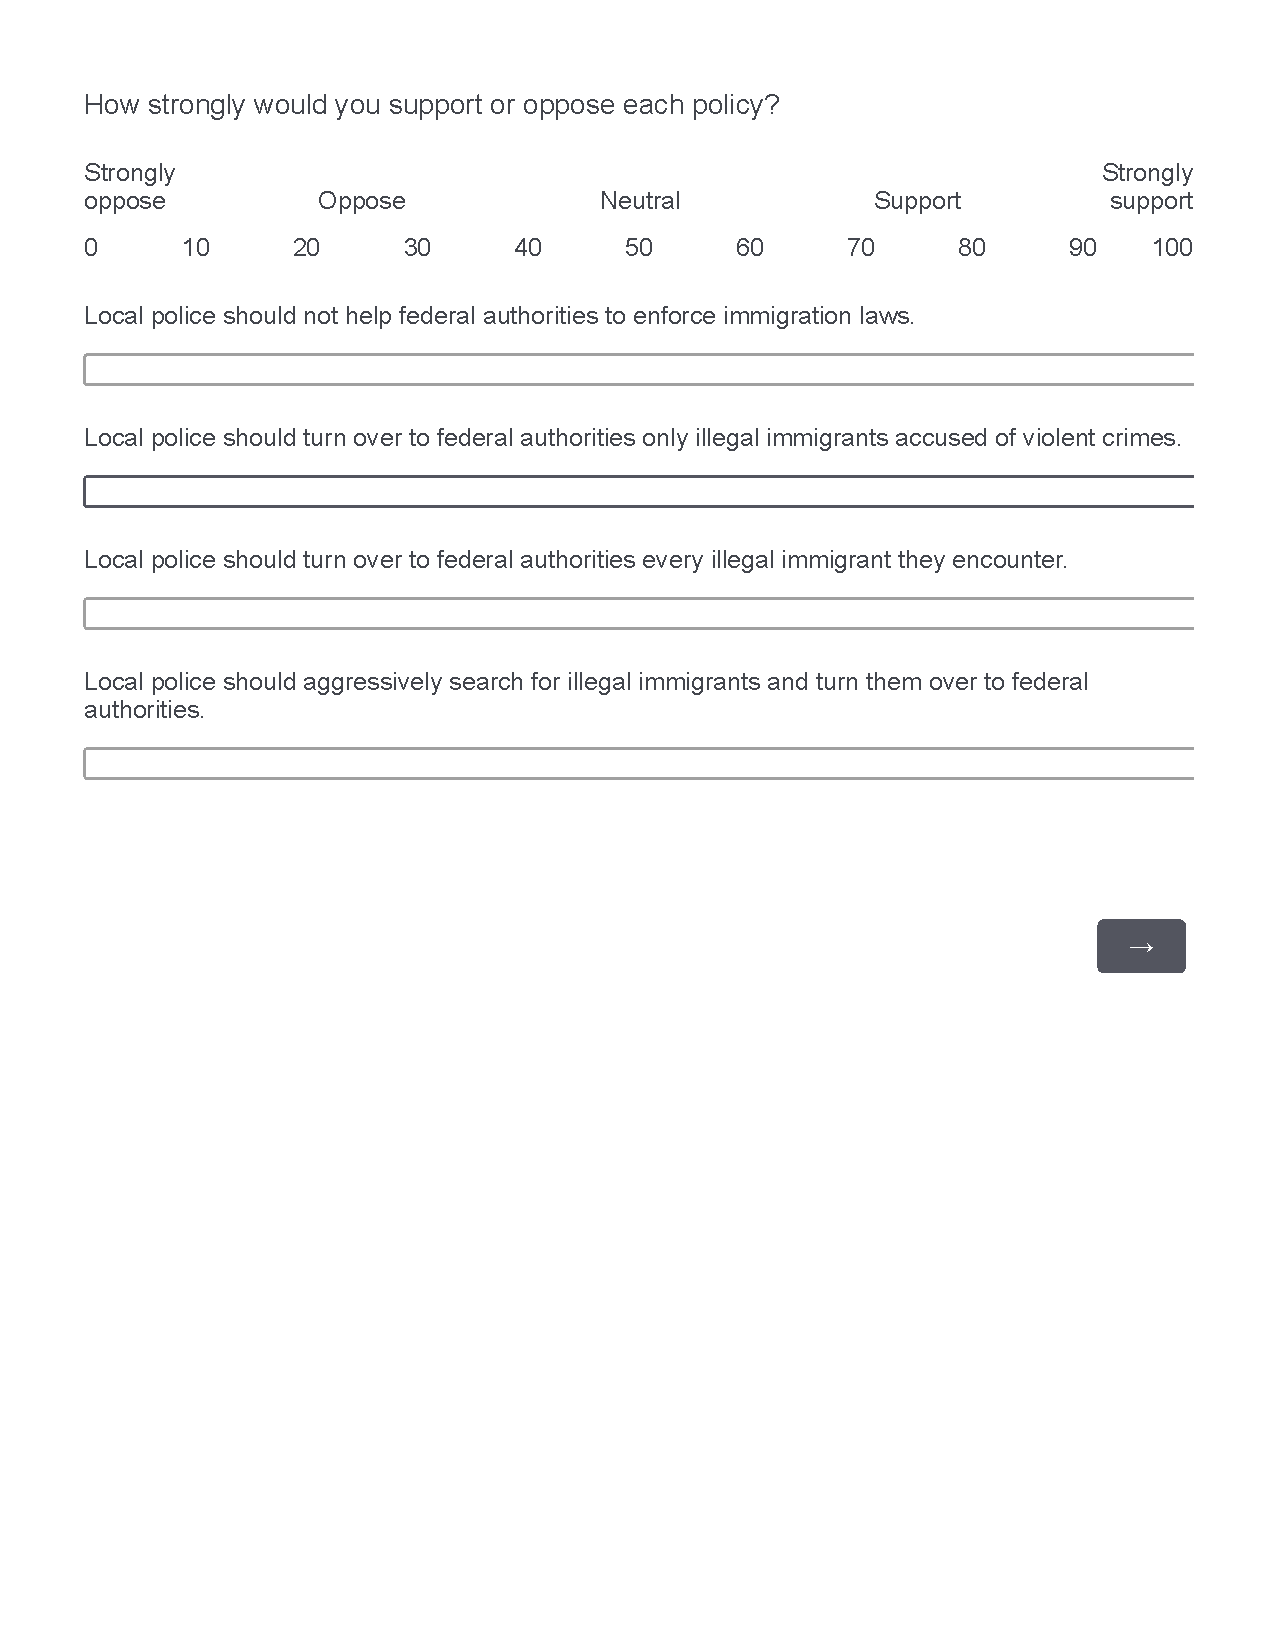
\includegraphics[width=\textwidth]{figures/appendix_survey_policyExample.pdf}
\end{figure}

\clearpage

\begin{figure}
\centering
\caption{Bundle rating instructions}
\vspace{4mm}
\label{fig:bundle_instruct}
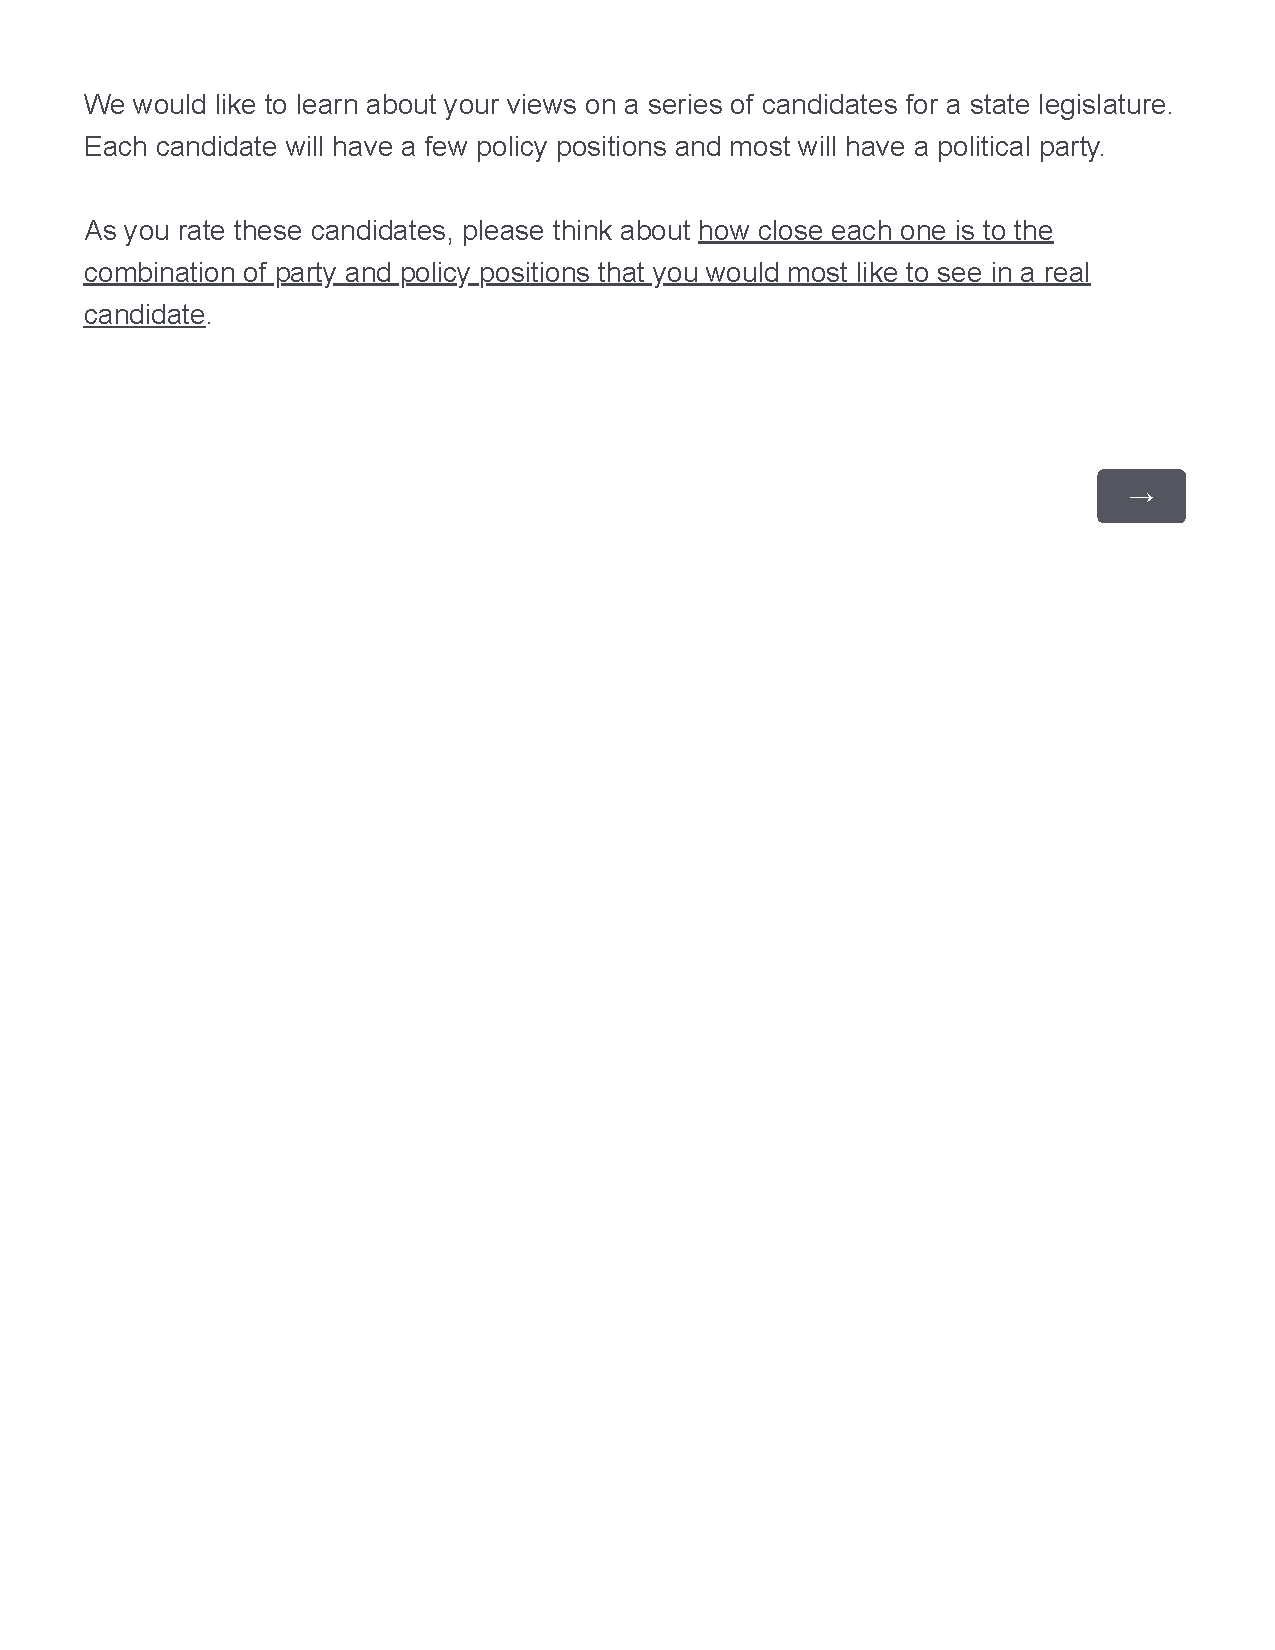
\includegraphics[width=\textwidth]{figures/appendix_survey_bundleInstruct.pdf}
\end{figure}

\begin{figure}
\centering
\caption{Bundle rating example}
\vspace{4mm}
\label{fig:bundle_example}
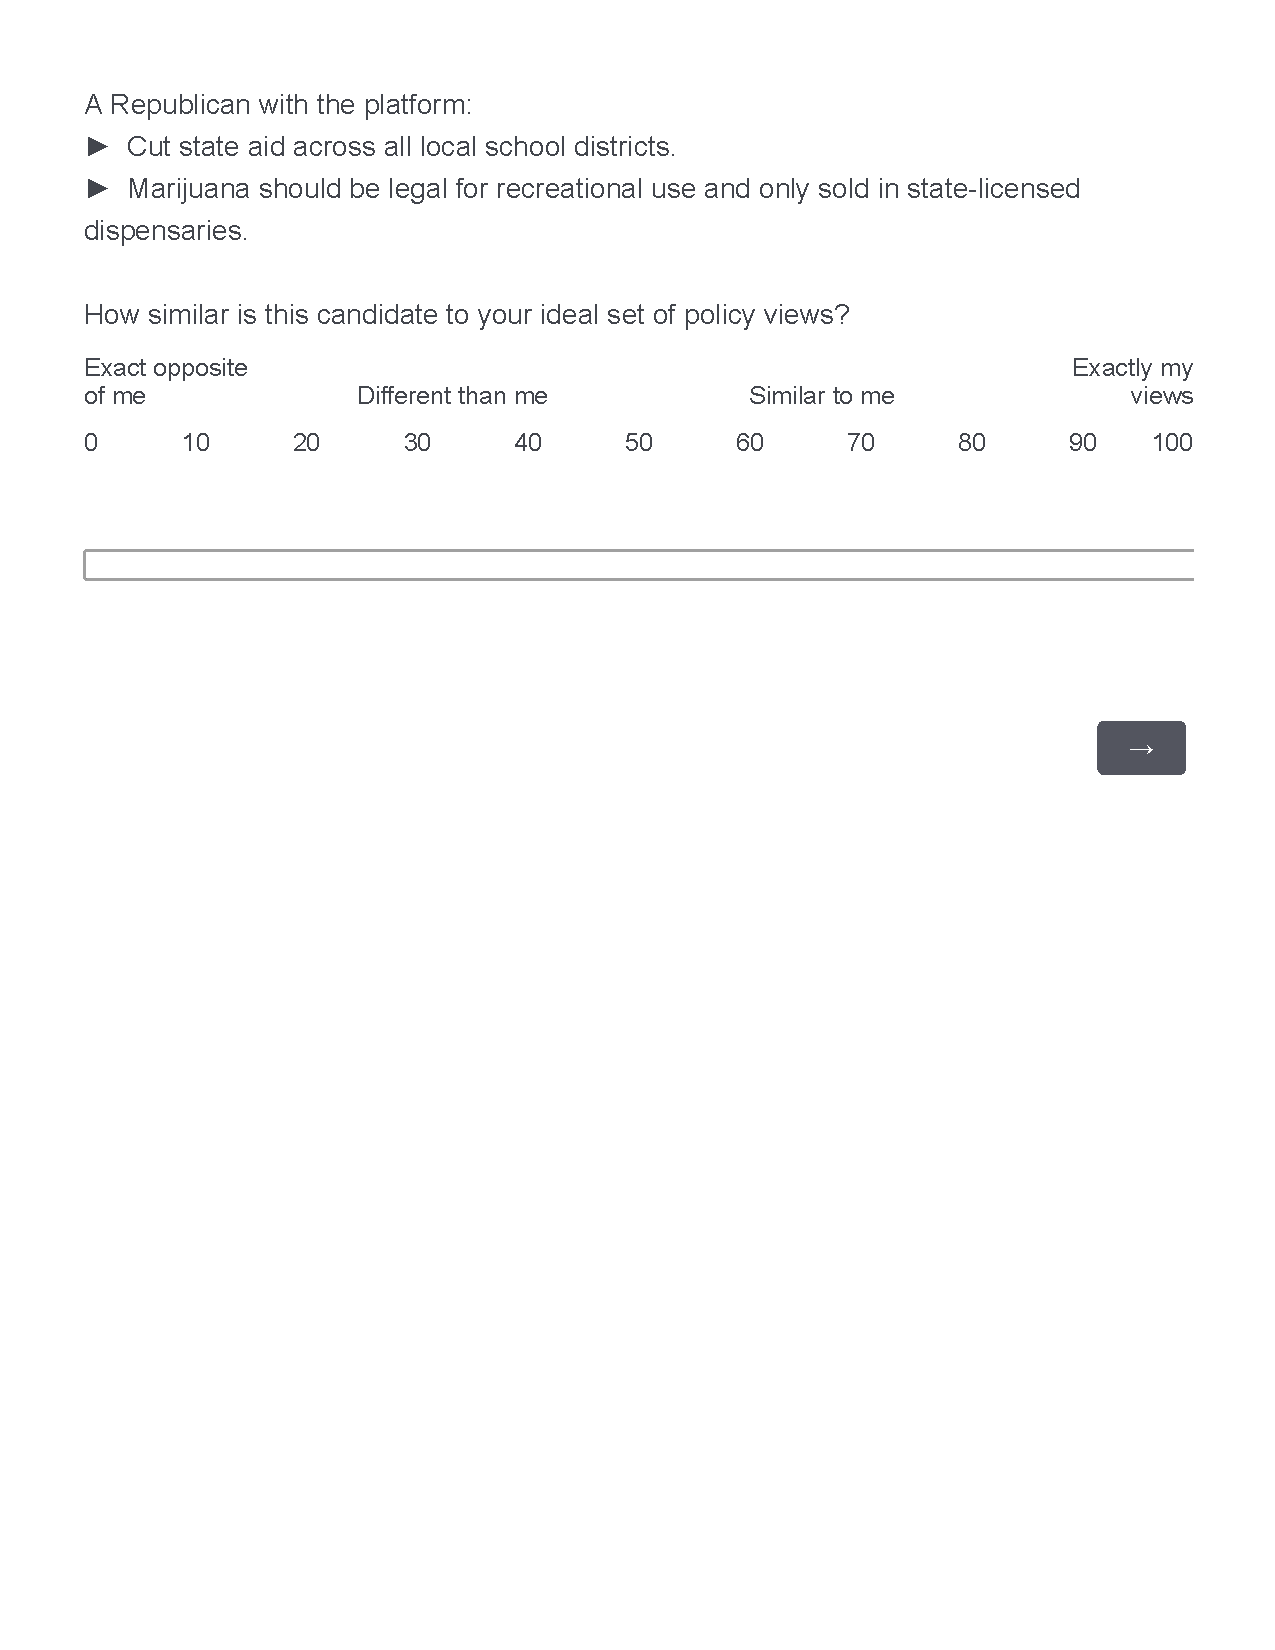
\includegraphics[width=\textwidth]{figures/appendix_survey_bundleExample.pdf}
\end{figure}

\clearpage

\begin{figure}
\centering
\caption{Candidate choice example}
\label{fig:cand_choice}
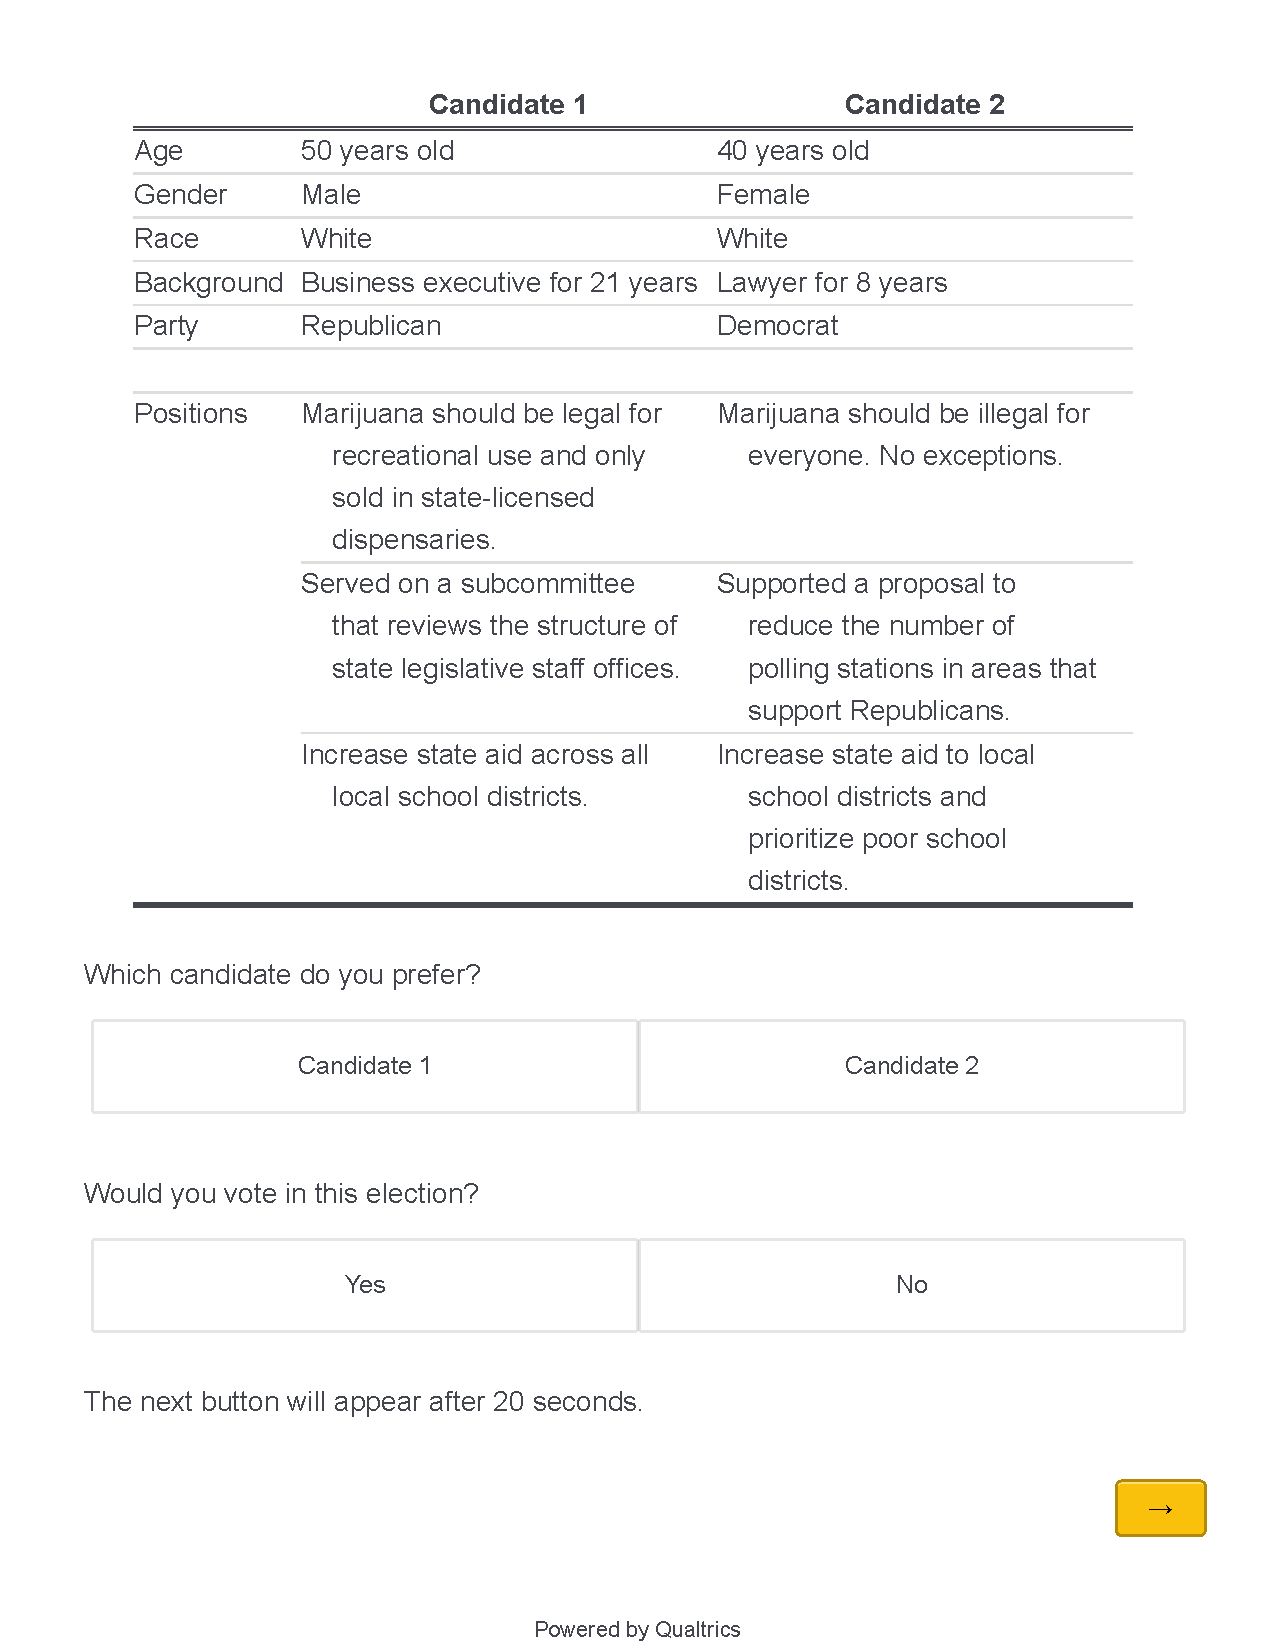
\includegraphics[width=\textwidth]{figures/appendix_survey_candChoice.pdf}
\end{figure}

\clearpage

\subsection{Candidate choices and the randomization procedure}

Each respondent made 16 candidate choices. All candidate characteristics were assigned by a combination of block random and simple random assignment. Figure~\ref{fig:cand_choice} presents an example of a candidate-choice scenario.

For all respondents, each candidate-choice scenario was assigned an ID number between 1 and 16. All attributes in scenarios 1 to 13 were assigned independently of the other. All candidates in scenarios 1 to 13 were either a Democrats or a Republican. In nine of these 13, one candidate endorsed one of seven undemocratic positions or committed one of two ``negative valence" behaviors; each of the nine negative attributes appeared once per respondent.

Candidate-choice scenarios 14 and 15 featured candidates without a political party, and scenario 16 was either a Democrat vs. Republican or Replican vs. Democrat choice in which both candidates were undemocratic. Because scenarios 14-16 did not use the same random assignment procedure as scenarios 1-13, our analysis excludes them unless explicitly noted.

Figure~\ref{fig:cand_attributes} lists the values of each attribute and the random assignment procedure. We selected the distribution of non-policy, non-democracy attributes using data from the National Council of State Legislatures, with an oversample of women and racial minorities. Note that although age and years of experience are not independent of one another, the possible combinations of age and years are independent of all other candidate characteristics.

\newpage

\newgeometry{left=2cm,bottom=3cm,top=2cm,right=1cm}
\begin{figure}
\caption{Randomization of candidate attributes}
\label{fig:cand_attributes}
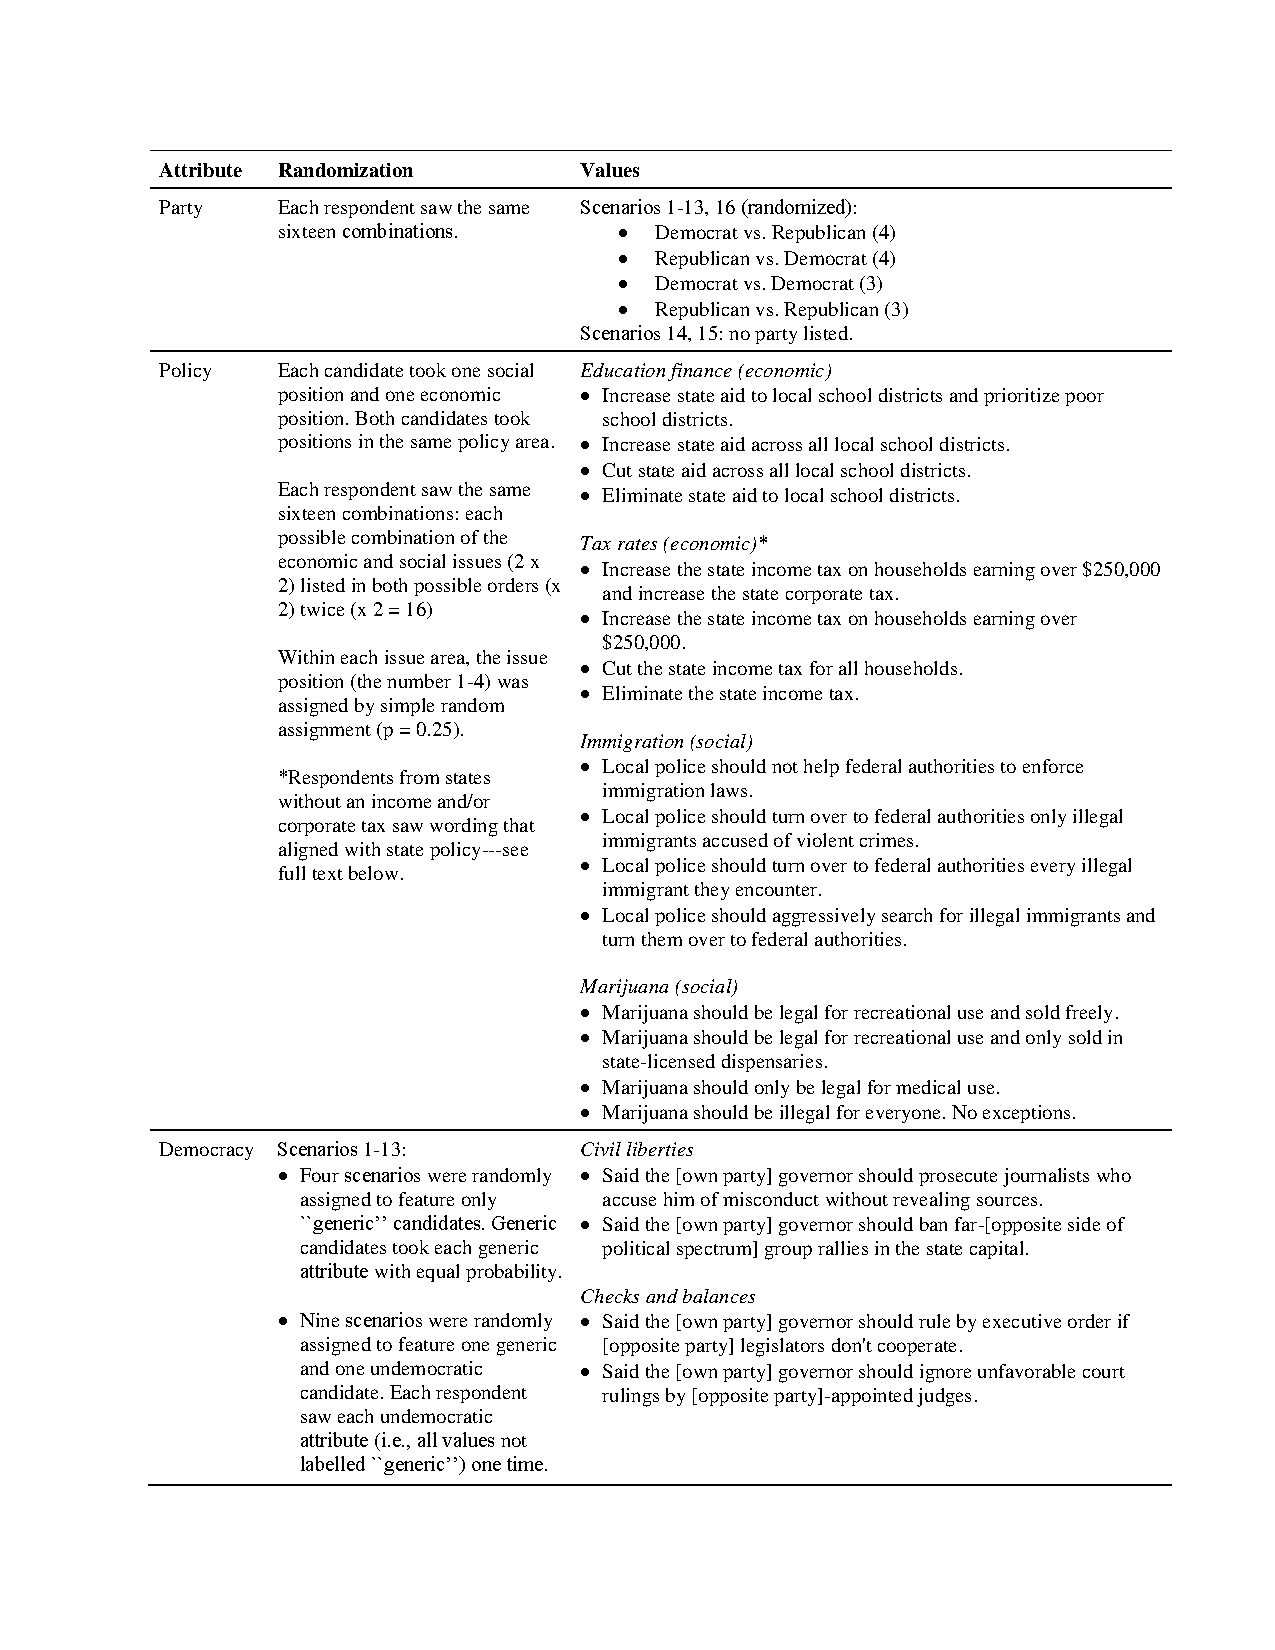
\includegraphics{figures/randomization_1.pdf}
\end{figure}
\clearpage
\newgeometry{left=1.5cm,bottom=3cm,top=2cm,right=1cm}
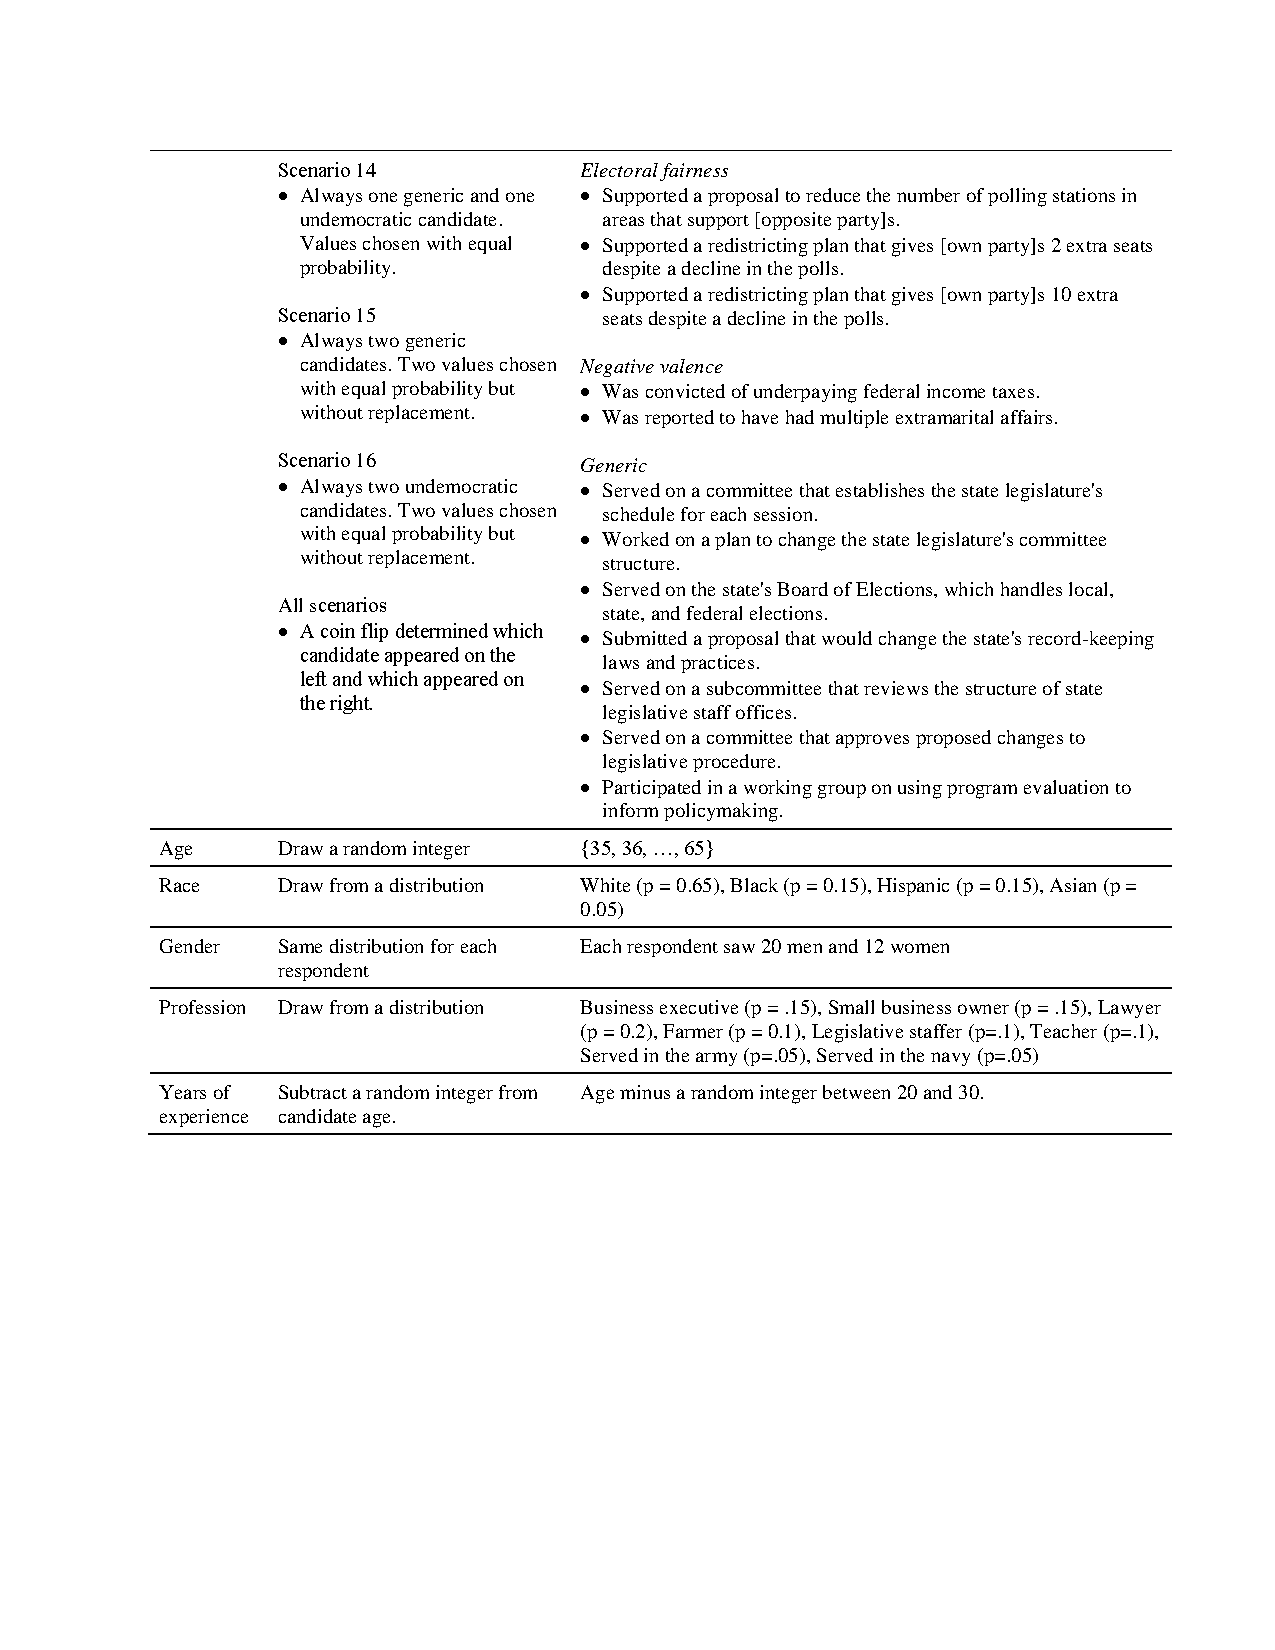
\includegraphics{figures/randomization_2.pdf}
\restoregeometry


\subsection{Justification of policy treatments\label{sec:policy}}

\onehalfspacing

We selected four policy areas---education, tax rates, immigration, marijuana---to be representative of the key economic and social policy issues in U.S. state politics. Both the \emph{Congressional Quarterly} (CQ) and the National Conference of State Legislatures (NCSL) included these four areas among their top policy areas for 2018.\footnote{CQ: Whit Robinson, ``\href{https://cgsnet.org/ckfinder/userfiles/files/CQState-11IssuesToWatch2018.pdf}{11 Issues to Watch in 2018},'' CQ State, January 2018. NCSL: Julia Lays, ``\href{http://www.ncsl.org/bookstore/state-legislatures-magazine/federalism-hot-legislative-issues-2018.aspx}{Top 10 in 2018},'' State Legislatures Magazine, January 2018.} In a 2016 survey of political reporters, CQ found that budget/taxes and education were the top two state public policy issues.\footnote{Ann Dermody, ``\href{https://info.cq.com/resources/top-public-policy-issues-each-state/}{52 Statehouse Reporters Review the Top 5 Public Policy Issues in Each State in 2016},'' CQ, May 3, 2016.} This section describes the substantive rationale for our choices in each area.

\vspace{2mm}

\textit{Education} is the largest budget item in U.S. states.\footnote{``\href{https://www.urban.org/policy-centers/cross-center-initiatives/state-local-finance-initiative/projects/state-and-local-backgrounders/state-and-local-expenditures}{State and Local Expenditures},'' Urban Institute backgrounder, accessed October 25, 2018.} According to the latest data from the National Center for Education Statistics, 45.1 percent of public school districts' 2013-14 revenue came from state aid, 46.5 percent from local sources, and 8.4 percent from the federal government.\footnote{Calculated using data from the National Center for Education Statistics (NCES) \href{https://nces.ed.gov/edfin/search/advanced.asp}{Public School District Finance Peer Search} on October 25, 2018.} As local revenue sources (chiefly property taxes) tend to be strongly tied to wealth and income, state aid to local districts is the key redistributive lever in state education finance: poorer districts count on it for a larger share of their budgets.\footnote{We confirmed this well-known relationship in the NCES data using the OLS regression
\vspace{-1mm}
\begin{center}
StateRevenuePercent$_i = s_i + \beta~$PercentPoverty$_i + \epsilon_i$
\end{center}
\vspace{-1mm}
where $i$ indexes school districts, StateRevenuePercent$_i$ is the percentage of the districts revenue that comes from the state, $s_i$ is a state fixed effect, and PercentPoverty$_i$ is the poverty rate among students. $\beta = 0.56$ (robust SE = 0.02), indicating that controlling for state-to-state average differences, each percentage point increase in the poverty rate among students predicts 0.56 percent greater budget share for state aid. These variable names match the source data from NCES.} We chose four policies that alter the level and distributive consequences of state aid. From most liberal to most conservative, the policies were:
\begin{itemize}
\setlength\itemsep{-.25em}
\singlespacing
\item Increase state aid to local school districts and prioritize poor school districts.
\item Increase state aid across all local school districts.
\item Cut state aid across all local school districts.
\item Eliminate state aid to local school districts.
\end{itemize}

\textit{Tax policy}. Sales, income, and corporate taxes are the largest revenue sources in U.S. state budgets.\footnote{``\href{https://www.urban.org/policy-centers/cross-center-initiatives/state-local-finance-initiative/projects/state-and-local-backgrounders/state-and-local-revenues}{State and Local Revenues},'' Urban Institute backgrounder, accessed October 25, 2018.} We designed four policies that would alter this revenue mix and its distributive consequences. Respondents in 41 states and the District of Columbia saw the following tax policies. Respondents in states lacking an income or sales tax saw slight modifications that fit the policies to the status quo in the state while preserving the left-right ordering of the policies; see the full survey text below.

\begin{itemize}
\setlength\itemsep{-.25em}
\singlespacing
\item Increase the state income tax on households earning over \$250,000 and increase the state corporate~tax.
\item Increase the state income tax on households earning over \$250,000.
\item Cut the state income tax for all households.
\item Eliminate the state income tax.
\end{itemize}

\textit{Immigration}. Many state policies affect unauthorized immigrants. One issue that is both salient and fundamental is the extent to which state and local law enforcement assist with enforcement of federal immigration laws. Because state and local police often come into contact with unauthorized immigrants but cannot themselves enforce immigration law, the federal government requests that local agencies hold them for pickup by federal authorities. Cities and states that do not fully cooperate are known as ``sanctuaries.'' We constructed a four-point scale of willingness to assist with federal immigration enforcement. We follow the ANES and CCES by referring to ``illegal'' immigrants.

\begin{itemize}
\setlength\itemsep{-.25em}
\singlespacing
\item Local police should not help federal authorities to enforce immigration laws.
\item Local police should turn over to federal authorities only illegal immigrants accused of violent crimes.
\item Local police should turn over to federal authorities every illegal immigrant they encounter.
\item Local police should aggressively search for illegal immigrants and turn them over to federal authorities.
\end{itemize}

\textit{Marijuana} has become an increasingly prominent state policy area since California became the first state to legalize medical marijuana 1996.\footnote{Sarah Trumble, ``\href{https://www.thirdway.org/infographic/timeline-of-state-marijuana-legalization-laws}{Timeline of State Marijuana Legalization Laws},'' \emph{Third Way}, April 19, 2017.} Today, marijuana is legal for recreational use in 10 states, for medical use in an additional 21, and in low-THC forms in another 15.\footnote{National Council of State Legislatures, ``\href{http://www.ncsl.org/research/health/state-medical-marijuana-laws.aspx}{State Medical Marijuana Laws},'' October 17, 2018.} As the trend in reform proposals and public opinion has been toward greater liberalization, our four-item set of marijuana policies is slightly to the left of status quo policy in the states: two recreational proposals (lax and stringent), a medical proposal, and an outright ban.

\begin{itemize}
\setlength\itemsep{-.25em}
\singlespacing
\item Marijuana should be legal for recreational use and sold freely.
\item Marijuana should be legal for recreational use and only sold in state-licensed dispensaries.
\item Marijuana should only be legal for medical use.
\item Marijuana should be illegal for everyone. No exceptions.
\end{itemize}

\clearpage
\newpage

\subsection{Measures of candidate-respondent policy distance\label{sec:altMeasures}}

\singlespacing

All results in the paper compute the distance between candidates and respondents using the respondent's average rating of the candidate's two policies. In this section we present results equivalent to those presented in the paper using alternative measures. We computed four measures of distance between candidates and respondents.
\begin{itemize}
\item \textbf{Policy rating}: The average of 0-100 rating of the candidate's two policies, based on the policy ratings described above.
\item \textbf{Policy rank}: Each respondent's policy ratings were transformed to the scale \{1, 2/3, 1/3, 0\}, ranging from favorite to least favorite.
\item \textbf{Party-policy bundle}: The 0-100 rating of the candidate's party and both policies, as described above.
\item \textbf{Ideological distance}: This measure is computed using the candidates' policies, the respondent's ideal policy, and a liberal-conservative ordering of the policies in each area.
\begin{itemize}
\item In each of the four policy areas, the four policies in each area were scored 1-4, from most liberal to most conservative.
\item The respondent's ideal policy in each policy area was identified based on their highest-rated policy. If two or more policies tied, the average was used as the ideal policy.
\item In each policy area, the difference between the candidate and the respondent was computed according to the formula $X_\text{respondent} - X_\text{candidate}$. This quantity was then averaged for the candidate's two policies.
\end{itemize}
\end{itemize}
For each of these four measures we applied two transformations common in formal theoretic analysis of electoral competition:
\begin{itemize}
\item \textbf{Absolute}: The untransformed rating, or negative absolute distance for the ideological measure.
\item \textbf{Squared}: The squared rating, or negative squared distance for the ideological measure.
\end{itemize}

For most of our results, we take the difference between Candidate 1 and Candidate 2's ratings on these measures. Table~\ref{tab:formulas} gives the formula for each measure and transformation: $R_{je}$ is the respondent's rating of the candidate $j$'s economic policy; $R_{js}$ is the social policy; $B_j$ is the party-policy bundle rating; rk() is the rank function; $x_{is}$ and $x_{ie}$ are respondent $i$'s ideal points on economic and social policy; and $x_{js}$ and $x_{je}$ are the ideological positions of candidate $j$'s policies.


\begin{table}[h]
\renewcommand{\arraystretch}{1.5}
\centering
\caption{Formulas used to calculate candidate 1's policy proximity advantage}
\vspace{2mm}
\label{tab:formulas}
\begin{tabular}{c l c c}
\hline
& & \multicolumn{2}{c}{Transformation} \\
\cline{3-4}
& & Absolute & Squared \\
\hline
\parbox[t]{2mm}{\multirow{8}{*}{\rotatebox[origin=c]{90}{~~Measure}}} & \\
&& \\[-8mm]
& ~~Policy proximity & $\frac{R_{1e} + R_{1s}}{2} - \frac{R_{2e} + R_{2s}}{2}$ & $(\frac{R_{1e}^2 + R_{1s}^2}{2}) - (\frac{R_{2e}^2 + R_{2s}^2}{2})$ \\
&&& \\[-4mm]
& ~~Policy rank & $\frac{\text{rk}(R_{1e}) + \text{rk}(R_{1s})}{2} - \frac{\text{rk}(R_{2e}) + \text{rk}(R_{2s})}{2}$ & $\frac{\text{rk}(R_{1e})^2 + \text{rk}(R_{1s})^2}{2} - \frac{\text{rk}(R_{2e})^2 + \text{rk}(R_{2s})^2}{2}$ \\
&&& \\[-4mm]
& ~~Party-policy bundle & $B_1 - B_2$ & $(B_1)^2 - (B_2)^2$\\
&&& \\[-4mm]
& ~~Ideological distance & $ \vert\frac{(x_{ie} - x_{2e}) + (x_{is} - x_{2s})}{2}\vert$ & $\frac{(x_{ie} - x_{2e})^2 + (x_{is} - x_{2s})^2}{2}$\\[-1mm]
& & ~~~~~~ $-\vert\frac{(x_{ie} - x_{1e}) + (x_{is} - x_{1s})}{2}\vert$ & ~~~~~~$-\frac{(x_{ie} - x_{1e})^2 + (x_{is} - x_{1s})^2}{2}$ \\
&&& \\[-4mm]
\hline
\end{tabular}
\end{table}

In the paper, we always use the formula in the top right cell of Table~\ref{tab:formulas}. The robustness checks below use the measures in the other seven cells. Figure~\ref{fig:density_full} plots the distribution of each measure (columns) and transformation (rows), with each colored line representing a different category of partisan strength (0 = independent, 1 = lean toward a party, 2 = partisan but not strong, 3 = strong partisan). Figure~\ref{fig:density_zoom} is identical except that the Y-axis is cut off so as to make differences in the distributions more evident. 

Note that while all distributions are similar, the rank-based distributions are almost identical. This is because by construction, the rank-based measure is distributed identically for every respondent. On this measure, differences between partisan groups can only emerge a consequence of chance variation in the candidate choices.

Table~\ref{tab:ks} tests the difference in the plotted distributions using the Kolmogorov-Smirnov test, a non-parametric test based on the largest difference between two empirical cumulative distribution functions. Note that the policy rank measure always passes the test, with the smallest $p=0.695$.

\begin{landscape}
\begin{figure}
\label{fig:density_full}
\caption{Density of policy distance measures by partisan strength}
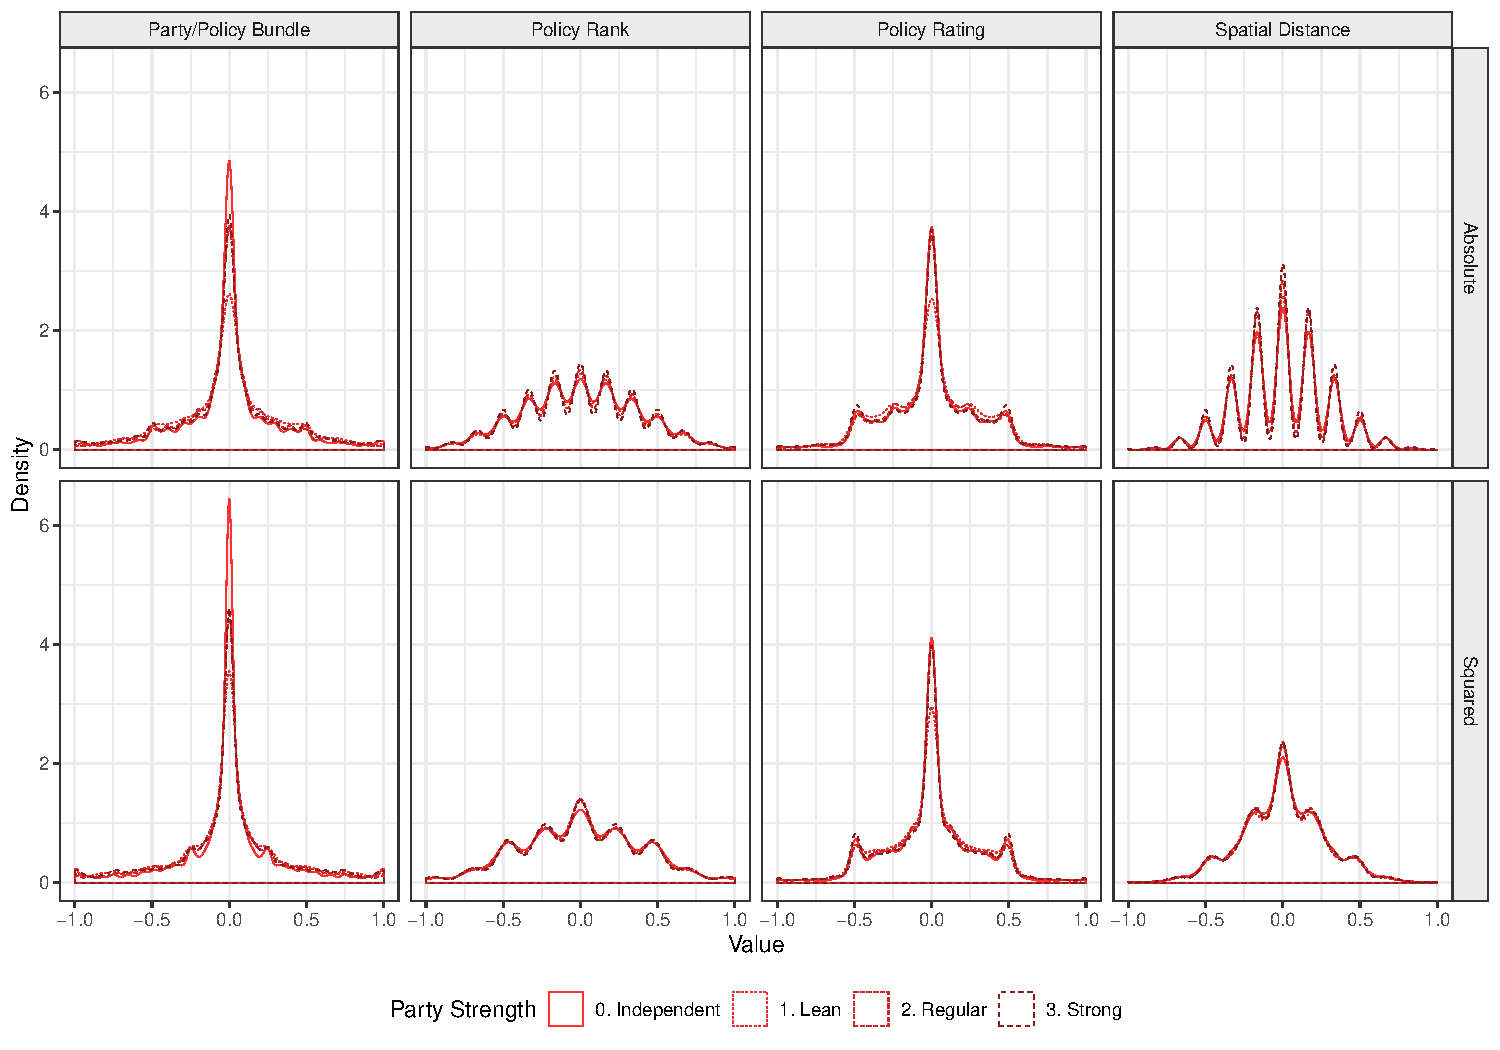
\includegraphics{figures/appendix_densityFull.pdf}
\end{figure}

\begin{figure}
\label{fig:density_zoom}
\caption{Density of policy distance measures by partisan strength, zoomed in on bottom}
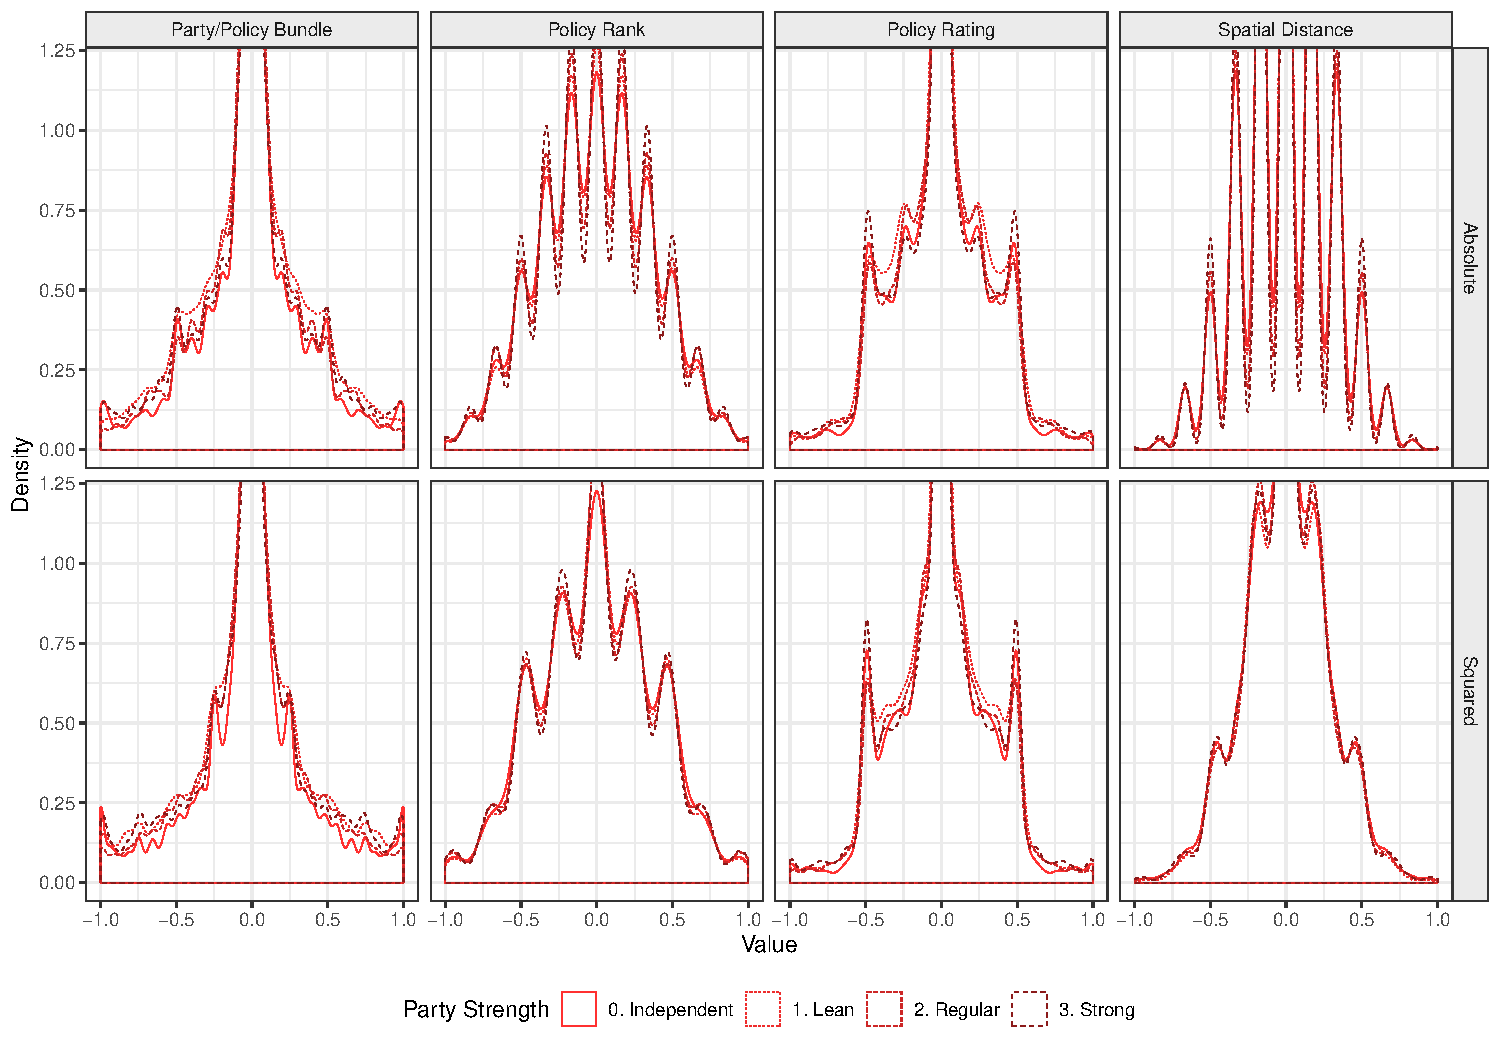
\includegraphics{figures/appendix_densityZoom.pdf}
\end{figure}
\end{landscape}

\begin{table}
\footnotesize
\caption{Kolmogorov-Smirnov test between party strength groups, by policy distance measure}
\vspace{2mm}
\label{tab:ks}
\input{figures/appendix_KStest.txt}
\end{table}

\clearpage

\subsection{Comparison to Census and ANES}

\onehalfspacing

The following tables compare respondents from our Lucid sample to the 2016 American National Election Study (ANES) web sample and the 2017 American Community Survey (ACS)\footnote{In 2010, the ACS replaced the long-form Census for all but a few population characteristics. As of this writing, the 2017 ACS one-year summary file is the most recent edition of the ACS.} one-year estimates for adult U.S. citizens. The first table displays partisanship and demographic characteristics from the Lucid sample, ANES, and ACS. The second displays a series of attitudinal and political knowledge variables that appear only in the Lucid and ANES surveys.

With one exception, the ACS data are individual-level estimates computed using the Public Use Microdata File. The ACS household income estimates are from the American FactFinder table S1901.\footnote{Shortly before publication, the Census Bureau announced the retirement of the American FactFinder. We regret any difficulty verifying the contents of this table.} Because the Lucid data are at the individual level, these estimates are not strictly comparable.

To make the sample more nationally representative, we computed raked weights using the ACS crosstabs below and the \texttt{survey} package in \texttt{R}. We trimmed the weights to fall between 1/2 and 2, then scaled them up so that they sum to the sample size. All results presented in the paper and this appendix use these weights. 

All ANES variables in the table below are computed using the weights that correspond to the survey wave in which the question was fielded. No ANES variables were used to construct the weights.

\singlespacing

\input{figures/appendix_benchmark_demog.txt}
\input{figures/appendix_benchmark_attitudes.txt}

\clearpage
\newpage

%%%%%%%%%%%%%%%%%%%%%%%%%%%%%%%%%%%%%%%%%
%%%%%%%%%%%%%%%%%%%%%%%%%%%%%%%%%%%%%%%%%



%%%%%%%%%%%%%%%%%%%%%%%%%%%%%%%%%%%%%%%%%%
%%%%%%%%%%%%%%%%%%%%%%%%%%%%%%%%%%%%%%%%%%

\section{Supporting Survey Results by Section}
\setcounter{figure}{0} 
\setcounter{table}{0} 

\subsection{Democratic Principles versus Policy Preferences}

For the ``Democratic Principles versus Policy Preferences'' section, we present three main sets of supplemental results:

\begin{itemize}
\item we reproduce the left and right panels of Figure 2 using several alternative measures of distance between the candidates' policies and our respondents' preferences;
\item we present numerical results that correspond to each point plotted in both panels, for both the policy distance measure used in the paper and each of the alternative measures of distance;
\item we reproduce the left panel separately for each democracy treatment.
\end{itemize}

\begin{landscape}
\newgeometry{left=2cm,bottom=1cm,top=2cm,right=-3cm}
\subsubsection{Figure 2, left panel with alternative measures\label{sec:fig1}}
This figure displays the analogue of Figure 2 in the paper. The first facet is identical to Figure 1 and the remaining facets use the alternative measures of candidate 1's proximity advantage described in Section~\ref{sec:altMeasures}.

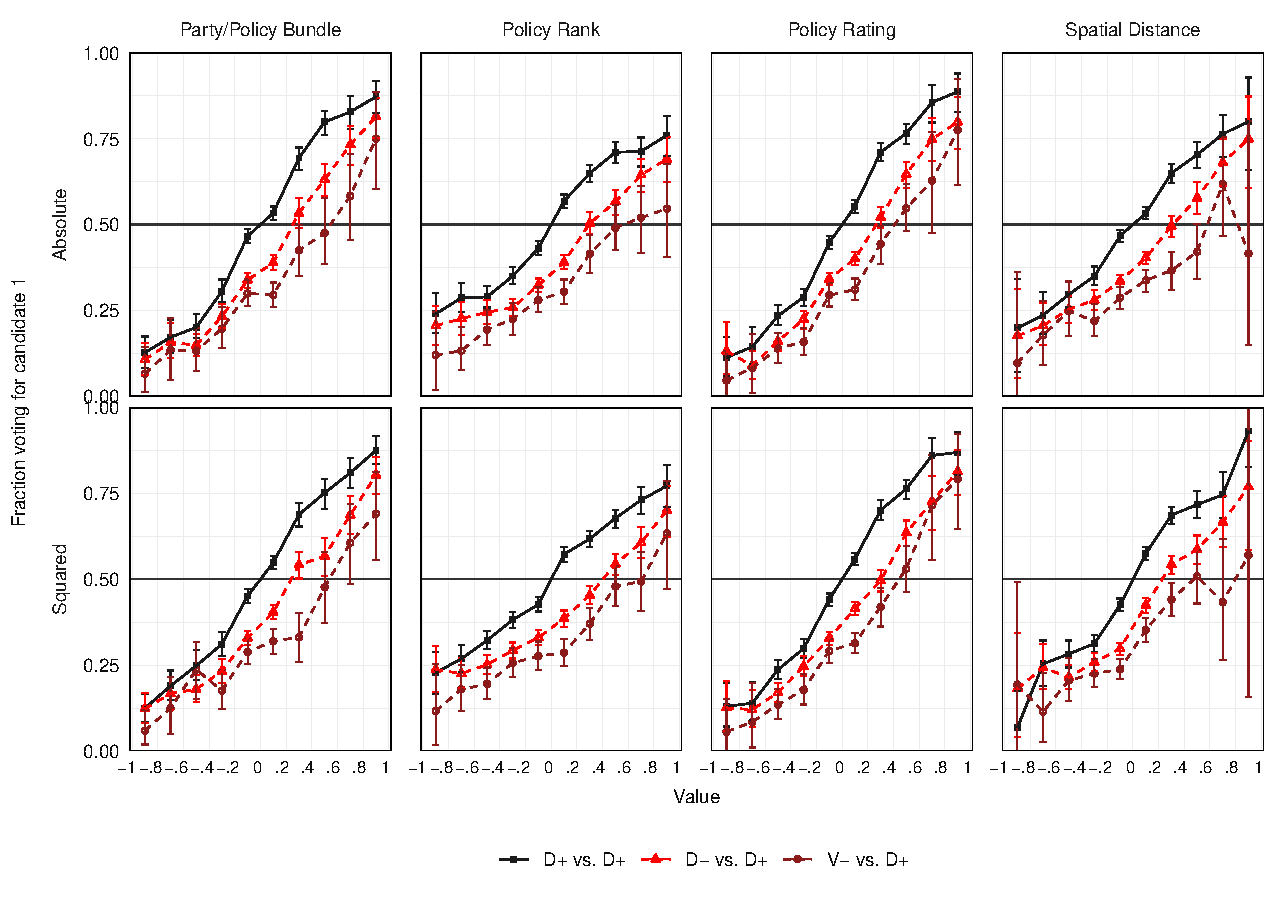
\includegraphics[width=.9\textwidth]{figures/appendix_fig2a_allMeasures.pdf}


\newpage

\subsubsection{Figure 2, right panel with alternative measures}
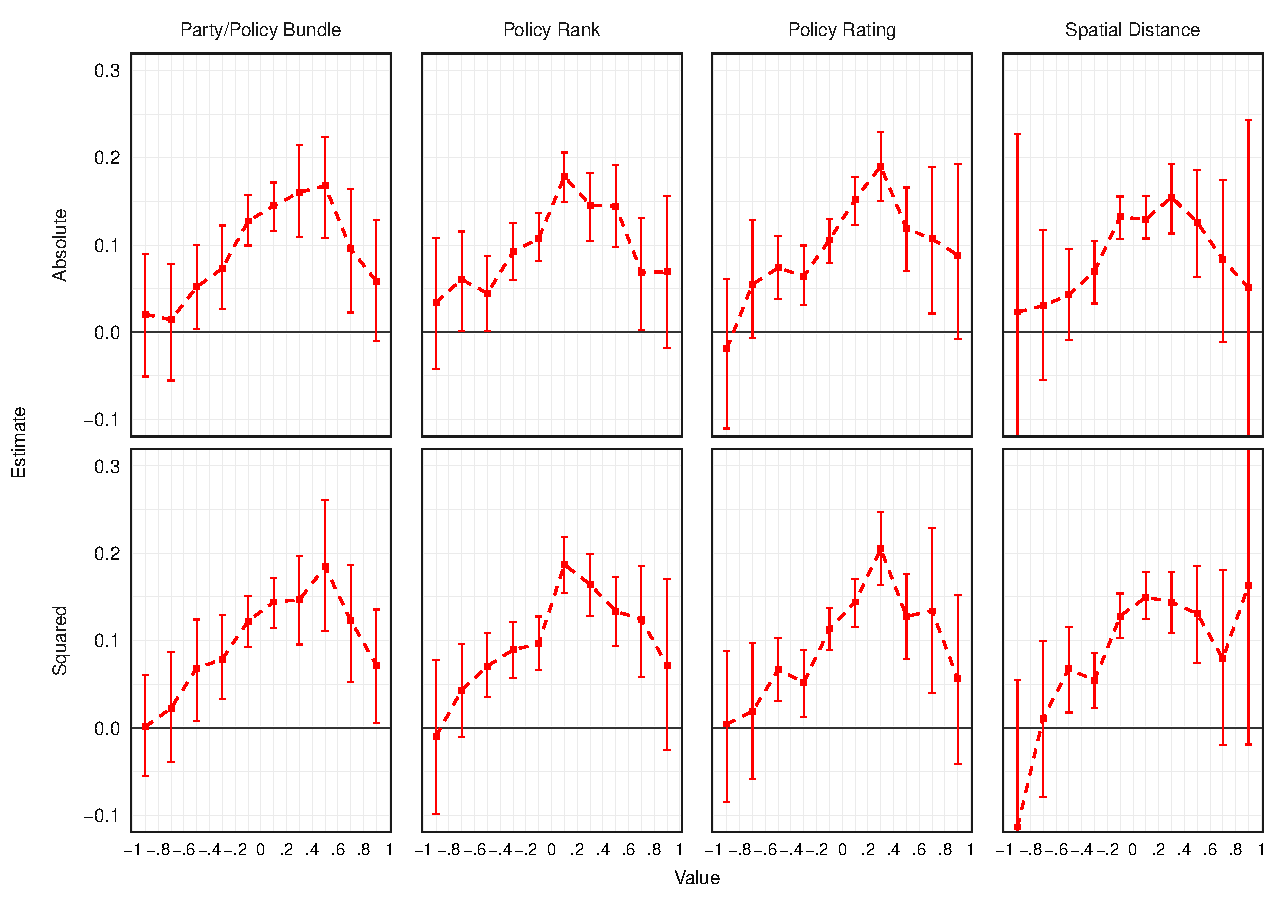
\includegraphics[width=.9\textwidth]{figures/appendix_fig2b_allMeasures.pdf}

\restoregeometry
\end{landscape}


\subsubsection{Numerical results for Figure 2}

The tables below present numerical results for the two preceding figures. Table~\ref{tab:meanVote} list candidate~1's mean vote share (the left panel of Figure 2) and Table~\ref{tab:allATE} presents the differences in means (the right panel of Figure 2).

\bgroup
\scriptsize
\singlespacing

\begin{longtable}{llllrrccc}
\caption{Mean Vote Share by Distance Measure\label{tab:meanVote}} \\

\toprule
& & & & & \multicolumn{2}{c}{------ Bootstrap ------} & \multicolumn{2}{c}{------ Clustered ------} \\
Measure & Transformation & Type & Value & Estimate & SE & CI & SE & CI \\
\midrule
\endfirsthead
\caption{Mean Vote Share by Distance Measure (continued)} \\
\toprule
& & & & & \multicolumn{2}{c}{ ------ Bootstrap ------} & \multicolumn{2}{c}{------ Clustered ------} \\
Measure & Transformation & Type & Value & Estimate & SE & CI & SE & CI \\
\midrule
\endhead
\bottomrule
\endfoot
\input{figures/tab_fig2a.txt}
\bottomrule
\end{longtable}

\clearpage

\begin{longtable}{llllrrccc}
\caption{Average Treatment Effect by Distance Measure\label{tab:allATE}} \\
\toprule
& & & & & \multicolumn{2}{c}{------ Bootstrap ------} & \multicolumn{2}{c}{------ Clustered ------} \\
Measure & Transformation & Type & Value & Estimate & SE & CI & SE & CI \\
\midrule
\endfirsthead
\caption{Average Treatment Effect by Distance Measure (continued)} \\
\toprule
& & & & & \multicolumn{2}{c}{------ Bootstrap ------} & \multicolumn{2}{c}{------ Clustered ------} \\
Measure & Transformation & Type & Value & Estimate & SE & CI & SE & CI \\
\midrule
\endhead
\bottomrule
\endfoot
\input{figures/tab_fig2b.txt}
\bottomrule
\end{longtable}

\egroup

\clearpage



\subsubsection{Figure 2, left panel separated by $D^-$ treatment}

The following figures present the analogue of Figure 2 in the paper separately for each democracy treatment. Each figure corresponds to one of the alternative measures of candidate-respondent distance described in Section~\ref{sec:altMeasures}. In each figure, each panel corresponds to a different $D^-$ treatment.

The red text in each panel displays the overall average treatment effect. Note that from measure to measure, the estimates change slightly due to missing data for some measures. In particular, because we only elicited a party-policy bundle measure for three-fourths of the candidate choices, the ATE estimates in the party-policy bundle plots reflect only three-fourths of the data. The policy rank estimates depart slightly from the policy rating estimates because creating the policy rank variable requires respondents to rate all four policies in each area.

\begin{figure}[h]
\begin{addmargin}{-3em}
\centering
\caption{Candidate 1’s vote share by treatment, policy rating, absolute}
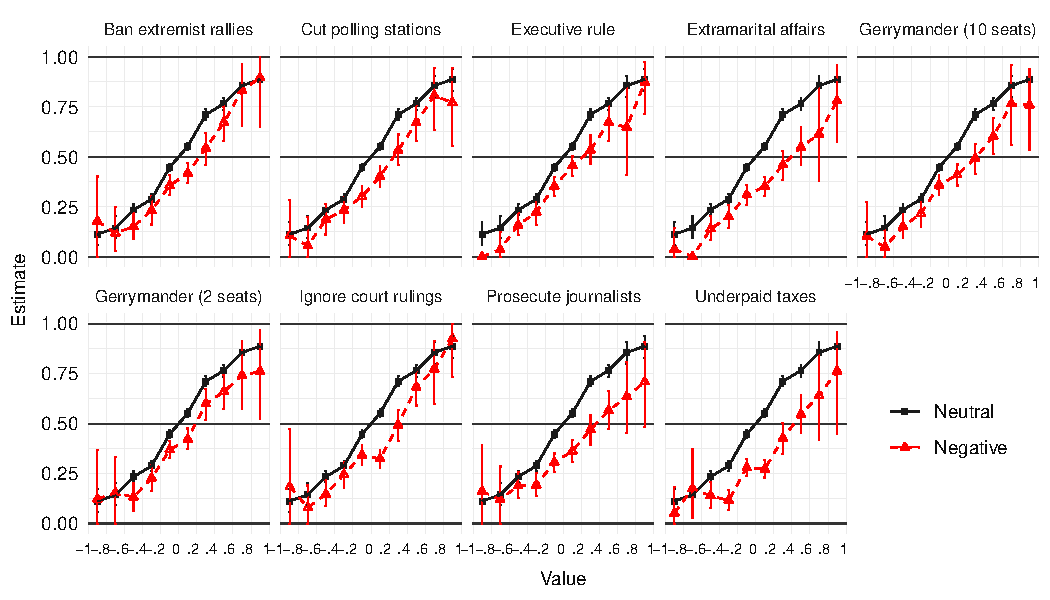
\includegraphics[width=1.1\textwidth]{figures/demByTrt_Policy_Rating_Absolute.pdf}
\end{addmargin}
\end{figure}

\begin{figure}[h]
\begin{addmargin}{-3em}
\centering
\caption{Candidate 1’s vote share by treatment, policy rating, squared}
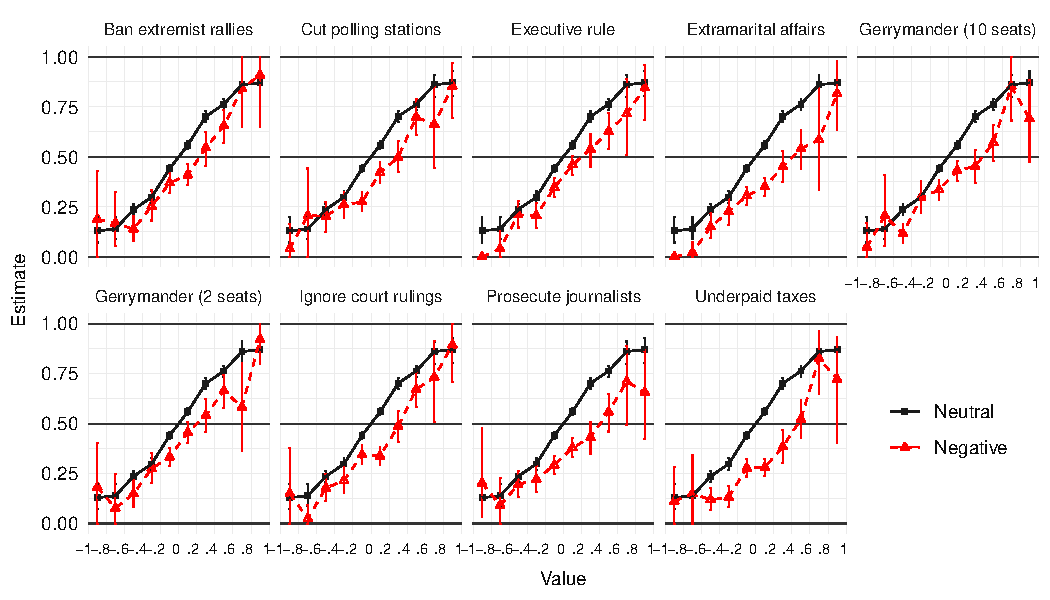
\includegraphics[width=1.1\textwidth]{figures/demByTrt_Policy_Rating_Squared.pdf}
\end{addmargin}
\end{figure}

\begin{figure}[h]
\begin{addmargin}{-3em}
\centering
\caption{Candidate 1’s vote share by treatment, policy rank, absolute}
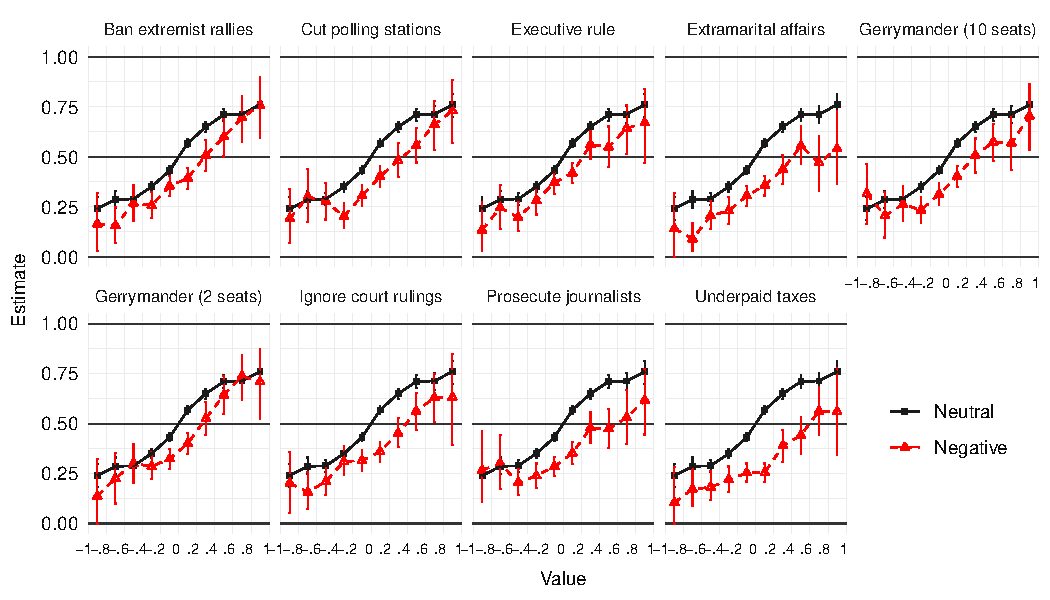
\includegraphics[width=1.1\textwidth]{figures/demByTrt_Policy_Rank_Absolute.pdf}
\end{addmargin}
\end{figure}

\begin{figure}[h]
\begin{addmargin}{-3em}
\centering
\caption{Candidate 1’s vote share by treatment, policy rank, squared}
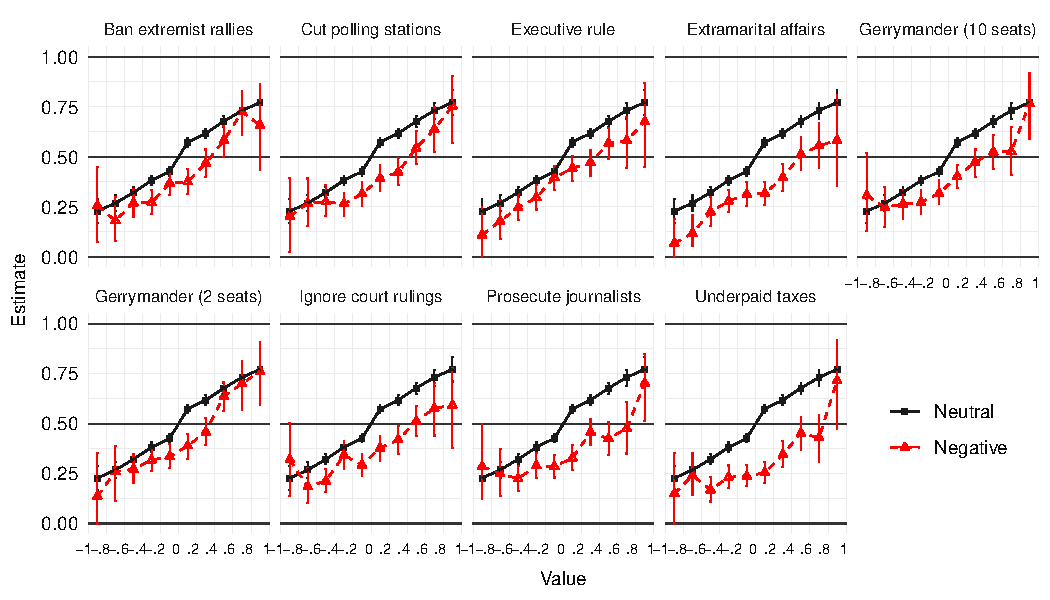
\includegraphics[width=1.1\textwidth]{figures/demByTrt_Policy_Rank_Squared.pdf}
\end{addmargin}
\end{figure}

\begin{figure}[h]
\begin{addmargin}{-3em}
\centering
\caption{Candidate 1’s vote share by treatment, party-policy bundle, absolute}
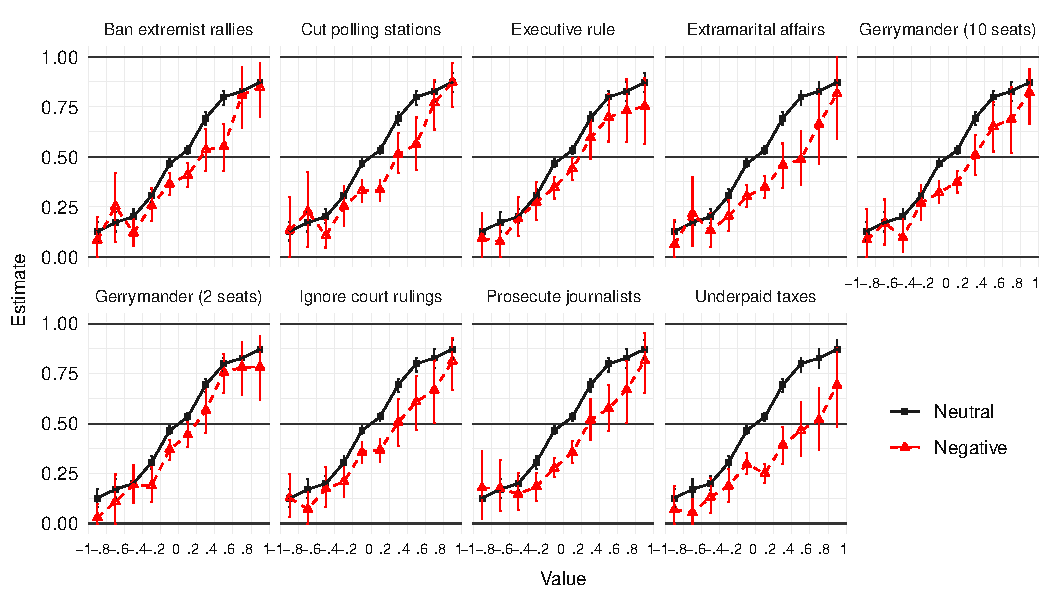
\includegraphics[width=1.1\textwidth]{figures/demByTrt_Party_Policy_Bundle_Absolute.pdf}
\end{addmargin}
\end{figure}

\begin{figure}[h]
\begin{addmargin}{-3em}
\centering
\caption{Candidate 1’s vote share by treatment, party-policy bundle, squared}
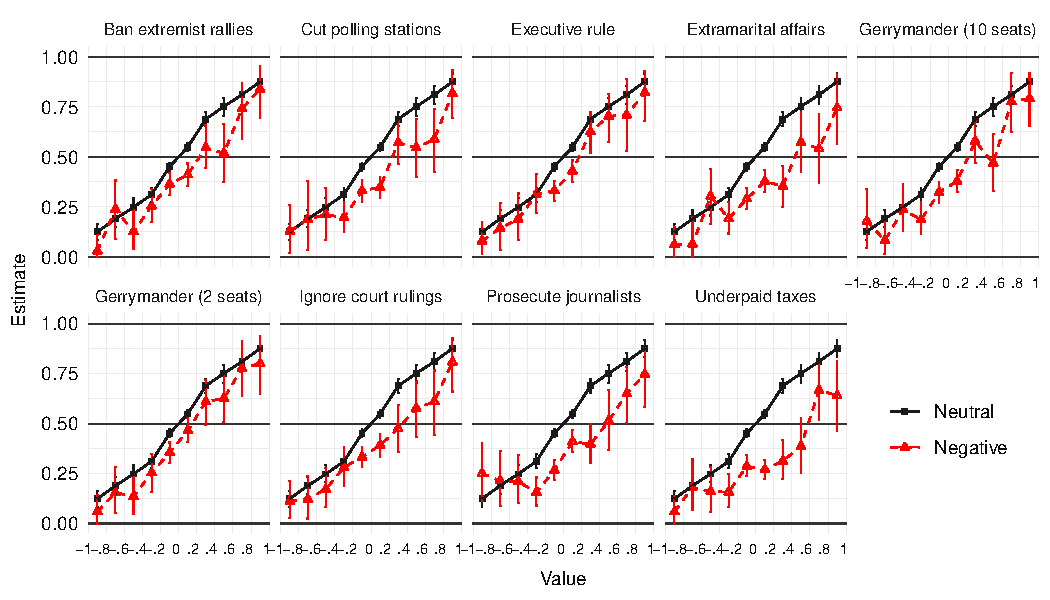
\includegraphics[width=1.1\textwidth]{figures/demByTrt_Party_Policy_Bundle_Squared.pdf}
\end{addmargin}
\end{figure}

\begin{figure}[h]
\begin{addmargin}{-3em}
\centering
\caption{Candidate 1’s vote share by treatment, ideological distance, absolute}
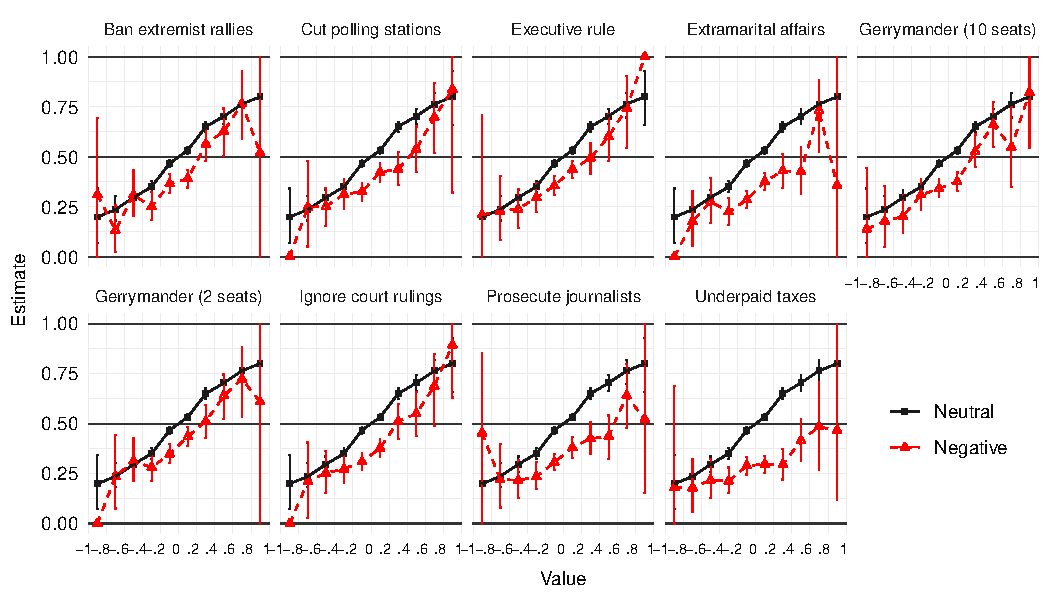
\includegraphics[width=1.1\textwidth]{figures/demByTrt_Spatial_Distance_Absolute.pdf}
\end{addmargin}
\end{figure}

\begin{figure}[h]
\begin{addmargin}{-3em}
\centering
\caption{Candidate 1’s vote share by treatment, ideological distance, squared}
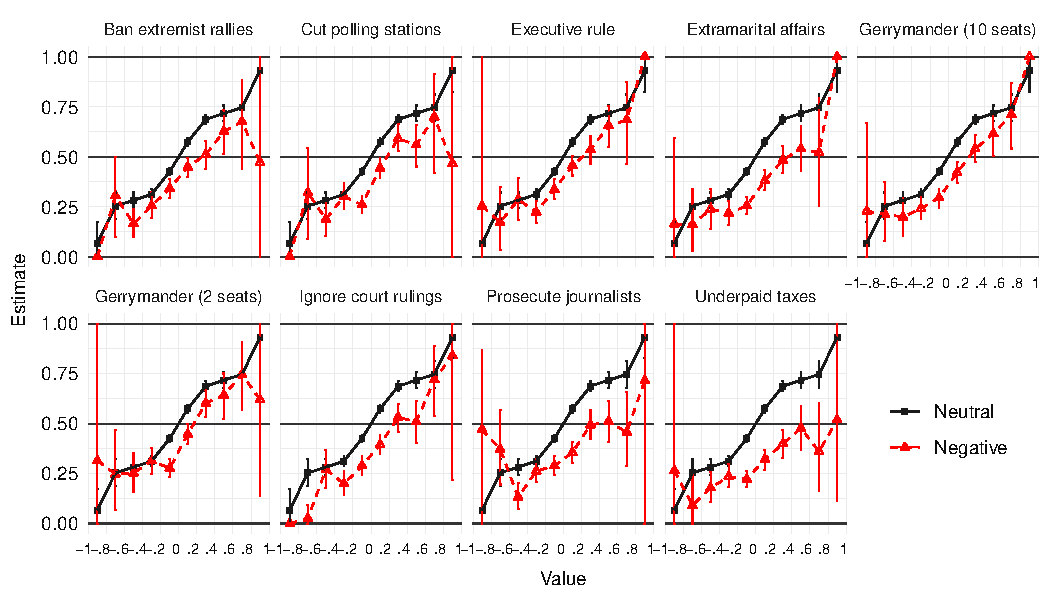
\includegraphics[width=1.1\textwidth]{figures/demByTrt_Spatial_Distance_Squared.pdf}
\end{addmargin}
\end{figure}

\clearpage

%%%%%%%%%%5

%%%%%%%%%%%%%%

\subsection{Does Partisanship Trump Civic Virtue?}

\subsubsection{Numerical results for Figures 3}

The following table corresponds to Figures 3 in the main text.

\input{figures/appendix_fig3_numerical.txt}

\clearpage
\newpage

\subsubsection{Numerical results and regression test for Figure 4}

The following table corresponds to Figures 4 in the main text.

\input{figures/appendix_fig4_numerical.txt}

~

\onehalfspacing

For a formal test of whether stronger partisans are less likely to punish $D^-$ candidates, we used OLS to estimate
$$ \mathbbm{1}(\text{Vote for Candidate 1})_{ij} = \beta_0 + \beta_1 (M_1-M_2)_{ij} + \beta_2 S_{i} + \beta_3 (M_1-M_2)_{ij} S_{i} + \epsilon_{ij}$$
where $i$ indexes respondents, $j$ indexes candidate choices, $M_1$ and $M_2$ are candidate 1 and 2's democracy positions, and $S$ measures partisan strength. We coded partisan strength \{0, 1, 2\} where 0 indicates leaners, 1 indicates weak partisans, and 2 indicates strong partisans. We excluded independents. 

To increase the precision with which we can estimate the relationship between strength of partisanship and willingness to punish for undemocratic candidates, we add controls for conduct the same test with controls for our respondents' preferences for same-party candidates, as well as the policy rank measure described in section~\ref{sec:altMeasures} (below, $P_1$-$P_2$). As explained there, the policy rank measure is orthogonal to all respondent characteristics by construction: within each policy area, each respondent's policy ratings were ranked so that every respondent's policy ratings take on the same uniform distribution (ties were broken randomly). Because the policy rank measure is correlated with the dependent variable, but uncorrelated by construction with any of the independent variables, including it leads to more precise estimates without introducing any confounding.

Table~\ref{tab:partyRegTest} displays the results, with robust standard errors clustered at the respondent level. The estimates of $\beta_3$ suggest that stronger partisans are less likely to punish a $D^-$ candidate.

\singlespacing

\input{figures/appendix_partyStrengthRegTest.txt}

\clearpage
\newpage

\subsubsection{Numerical results for Figure 5}

The following table corresponds to Figures 5 in the main text.

\input{figures/appendix_fig5_numerical.txt}

\clearpage

%%%%%%%%%%%%%%

\subsection{The Consequences of Candidate Polarization}

\subsubsection{Numerical results for Figure 6}

\input{figures/appendix_fig6_numerical.txt}

\subsubsection{Figure 6 robustness check}

The figure below displays two robustness checks for Figure 6 in the paper. Figure~\ref{fig:platform_real} presents the estimates from the paper (left panel) along with results that exclude scenarios in which the two candidates took the exact same position on either policy (right panel).

\begin{figure}[h]
\centering
\caption{Defection rate by candidate platform distance.\label{fig:platform_real}}
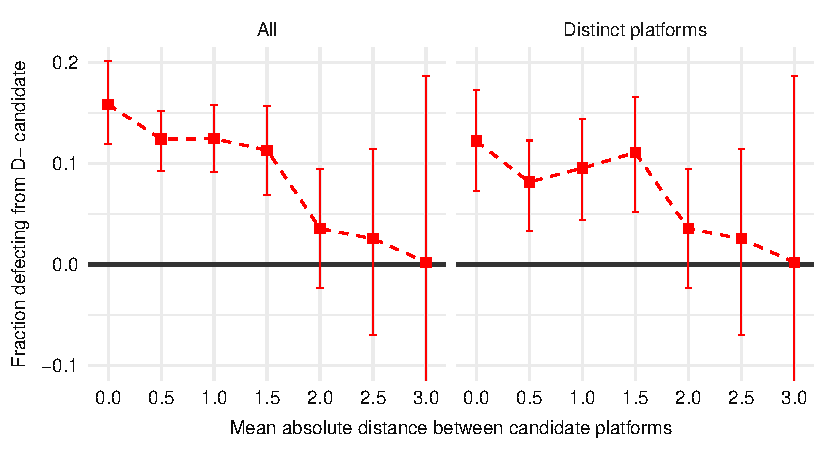
\includegraphics{figures/appendix_fig6_alternative.pdf}
\end{figure}

\newpage

\subsubsection{Regression test for heterogeneity}

For a formal test of whether defection is decreasing in platform distance, we used OLS to fit the linear model
$$ \mathbbm{1}(\text{Vote for Candidate 1})_{ij} = \beta_0 + \beta_1 (M_1-M_2)_{ij} + \beta_2 P_{ij} + \beta_3 (M_1-M_2) \times P_{ij} + \epsilon_{ij} $$
where $i$ indexes respondents, $j$ indexes candidate choices, $M_1$ and $M_2$ are candidate 1 and 2's democracy positions, and $P\equiv| \frac{P_{1E}-P_{2E} + P_{1S} - P_{2S}}{2} |$ is the mean absolute distance between candidate 1 and 2's policy positions on a left-right scale. As in the figure, this measure can take the values \{0, 0.5, 1, 1.5, 2, 2.5, 3\}. See section~\ref{sec:altMeasures} for details as to how we mapped the candidates' positions onto a left-right scale. 

The positive coefficient on $\beta_3$ constitutes evidence that when policy differences between candidates are larger, our respondents were less likely to punish a $D^-$ candidate.

\bgroup
\footnotesize
\input{figures/appendix_fig6_regression.txt}
\egroup

\clearpage
\newpage

\subsection{Resisting the Menu of Manipulation}

\subsubsection{Numerical results for Figures 7 and 8}

The following tables provide numerical results that correspond to Figures 7 and 8 in the paper.

To test whether there are statistically significant differences in how severely respondents punish the distinct D$^-$ positions, we conducted an F-test for the equality of all of the D$^-$ coefficients in Table~\ref{tab:AMCE}. We find that $F=3.8232$ (df = 6 and 18102, $p$ = 0.0008212).

To demonstrate that the choice between cluster-robust and block bootstrapped standard errors makes little difference, Table~\ref{tab:AMCE} includes standard errors computed by both methods. The correlation between the two sets of standard errors is 0.9988 and the average block bootstrapped standard error is 1.5 percent larger than the average clustered standard error.

\input{figures/appendix_fig7_numerical.txt}

\clearpage

\input{figures/appendix_fig8_numerical.txt}

\clearpage

\clearpage

\subsubsection{Estimation method}

\onehalfspacing

Here we clarify how we adapt the Average Marginal Component Effect (AMCE) framework (Hainmuller et al. 2015) to our experimental design. A key difference between the typical conjoint design and our candidate-choice experiment is that the former is most often based on the uniform randomization of all attributes at the candidate level. By contrast, (1) most of our candidate attributes were randomized to mirror the real-world distribution of those attribute among state legislators (i.e. not uniform), and (2) we intentionally constrained our randomization of democracy positions in the 13 (out of 16) candidate-choice scenarios that we focus on in the main text to feature either the $D^+ \text{ vs. } D^+$, $D^- \text{ vs. } D^+$, or $D^+ \text{ vs. } D^-$ conditions but not the $D^- \text{ vs. } D^-$ condition. The purpose of this constraint was to focus in the majority of our scenarios on the process of democratic backsliding and the public’s willingness to check it.\footnote{One of the remaining three scenarios did include the $D^- \text{ vs. } D^-$ condition; see Figure~\ref{fig:cand_attributes}.} That is, we treat the $D^+ \text{ vs. } D^+$ condition as a control reflecting the status quo and the $D^- \text{ vs. } D^+$ and $D^+ \text{ vs. } D^-$ conditions as treatments. 

To adapt the AMCE framework to our experimental design, we begin with a regression equation that gives separate estimates of the effects of candidate 1 and candidate 2's attributes:
\begin{align}
\mathbbm{1}(\text{choose candidate } 1) = \alpha + \sum_j \beta_j X_{1ij} + \sum_j \gamma_j X_{2ij} + \epsilon_{ij} \label{eq:trueAMCE}
\end{align}
where $X_{1ij}$ and $X_{2ij}$ are indicator variables for all possible values of attribute $j$ in choice $i$ between candidates 1 and 2. Because all attributes are balanced across the two candidates by randomization, the effect of $X_{1ij}$ and $X_{2ij}$ is the same for candidates 1 and 2. This implies that we can simplify the above formulation by $\beta_j=-\gamma_j$, giving
\begin{align}
\mathbbm{1}(\text{choose candidate } 1) = \alpha + \sum_j \beta_j (X_{1ij} - X_{2ij}) + \epsilon_{ij} \label{eq:AMCE}
\end{align}

Reporting estimates for (\ref{eq:AMCE}) allows us to present our results in the familiar AMCE style of one coefficient per attribute while staying true to our randomization procedure. In the paper, we presented these results using only the candidates' democracy positions.

In the main text, Figure 7 uses (\ref{eq:AMCE}) to compute results for the full range of candidate attributes, with the exception of candidate age and years of job experience. As described above, age and job experience are jointly randomized in our design, with 31 $\times$ 11 = 341 total possible values. Rather than display estimates for each possible age/experience combination, we treat these as background noise that is (by design) independent of all other candidate characteristics.

Table~\ref{tab:AMCE} presents numerical results that correspond to Figure~7, with both bootstrapped and cluster-robust standard errors. The two methods of estimating standard errors yield very similar results.

To validate the claim that $\beta_j = -\gamma_j$, Figure~\ref{fig:amce_both} displays results based on (\ref{eq:trueAMCE}). To facilitate the comparison of the coefficients, we multiply $\gamma_j$ by $-1$.\footnote{Note that differences between coefficient estimates for the two candidates may be a consequence of how our data is organized. Above and in the paper, we note that although candidates 1 and 2 were equally likely to appear as $D^-$ to the respondent, we reshaped our data so that candidate~1 varies between $D^-$ and $D^+$ (depending on the experimental condition), while candidate~2 serves as a reference candidate, always holding a neutral position ($D^+$). The smaller (negative) coefficient estimate for “different party’’ for candidate~1 is most likely the consequence of the partisan double standard that we examine in section 3 of the paper: partisans punish $D^-$ candidates from “different party” more severely than candidates from “same party”, and this only affects candidate~1 in our data. Such differences between coefficient estimates for the two candidates can be eliminated by including interaction terms capturing such partisan double standard (as we do in section 4 of the paper).}

\begin{figure}
\caption{Average marginal effect for candidate characteristics: separate estimates for both candidates}
\label{fig:amce_both}
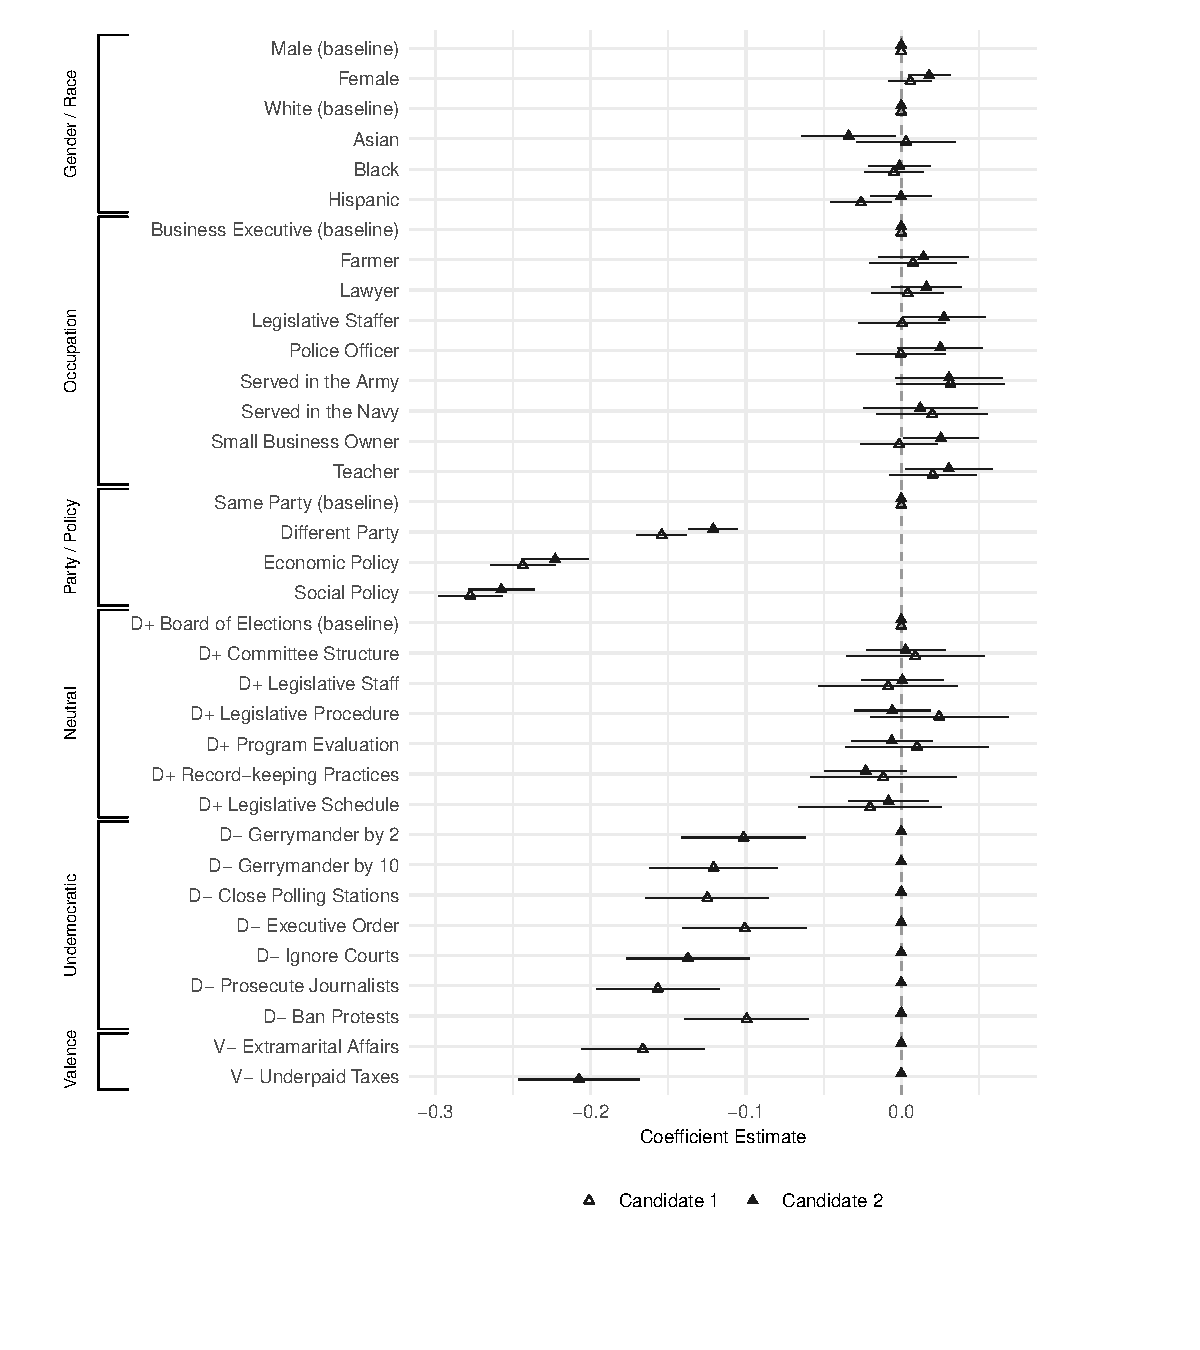
\includegraphics{figures/appendix_fig7_separated.pdf}
\end{figure}

\clearpage
\newpage



%%%%%%%%%%

\subsection{Structural Estimates of Support for Democracy}
\singlespacing

This subsection supplements our structural analysis with
\begin{itemize}
\item a graphical summary of the relationship among key structural parameters;
\item an assessment of the goodness of fit for the logit model;
\item full regression tables for the logit models that we used to compute the structural parameters.
\end{itemize}

\subsubsection{A summary of the relationship among key structural parameters}
\onehalfspacing

The relationship between the structural parameters estimated in this section of the paper is graphically summarized by Figure \ref{fig: mrs_plot}. It plots the combinations of economic and social policies that result in an equal probability of victory for both candidates, assuming candidate~1 is the respondent's co-partisan but candidate~2 is not. We refer to these lines as \emph{isoelects}. The solid black isoelect plots combinations of economic and social policies that result in an equal probability of victory for either candidate when both adopt a neutral democracy position ($D^+ \text{ vs. } D^+$); the dashed blue and dotted red isoelects correspond to the $D^- \text{ vs. } D^+$ and $D^+ \text{ vs. } D^-$ conditions, respectively. Combinations of economic and social policies to the right and above the isoelects correspond to scenarios when candidate~1 is more likely to win; policy combinations to the left and below the isoelects correspond to scenarios when candidate~2 is more likely to win.

\begin{figure}[h]
\center
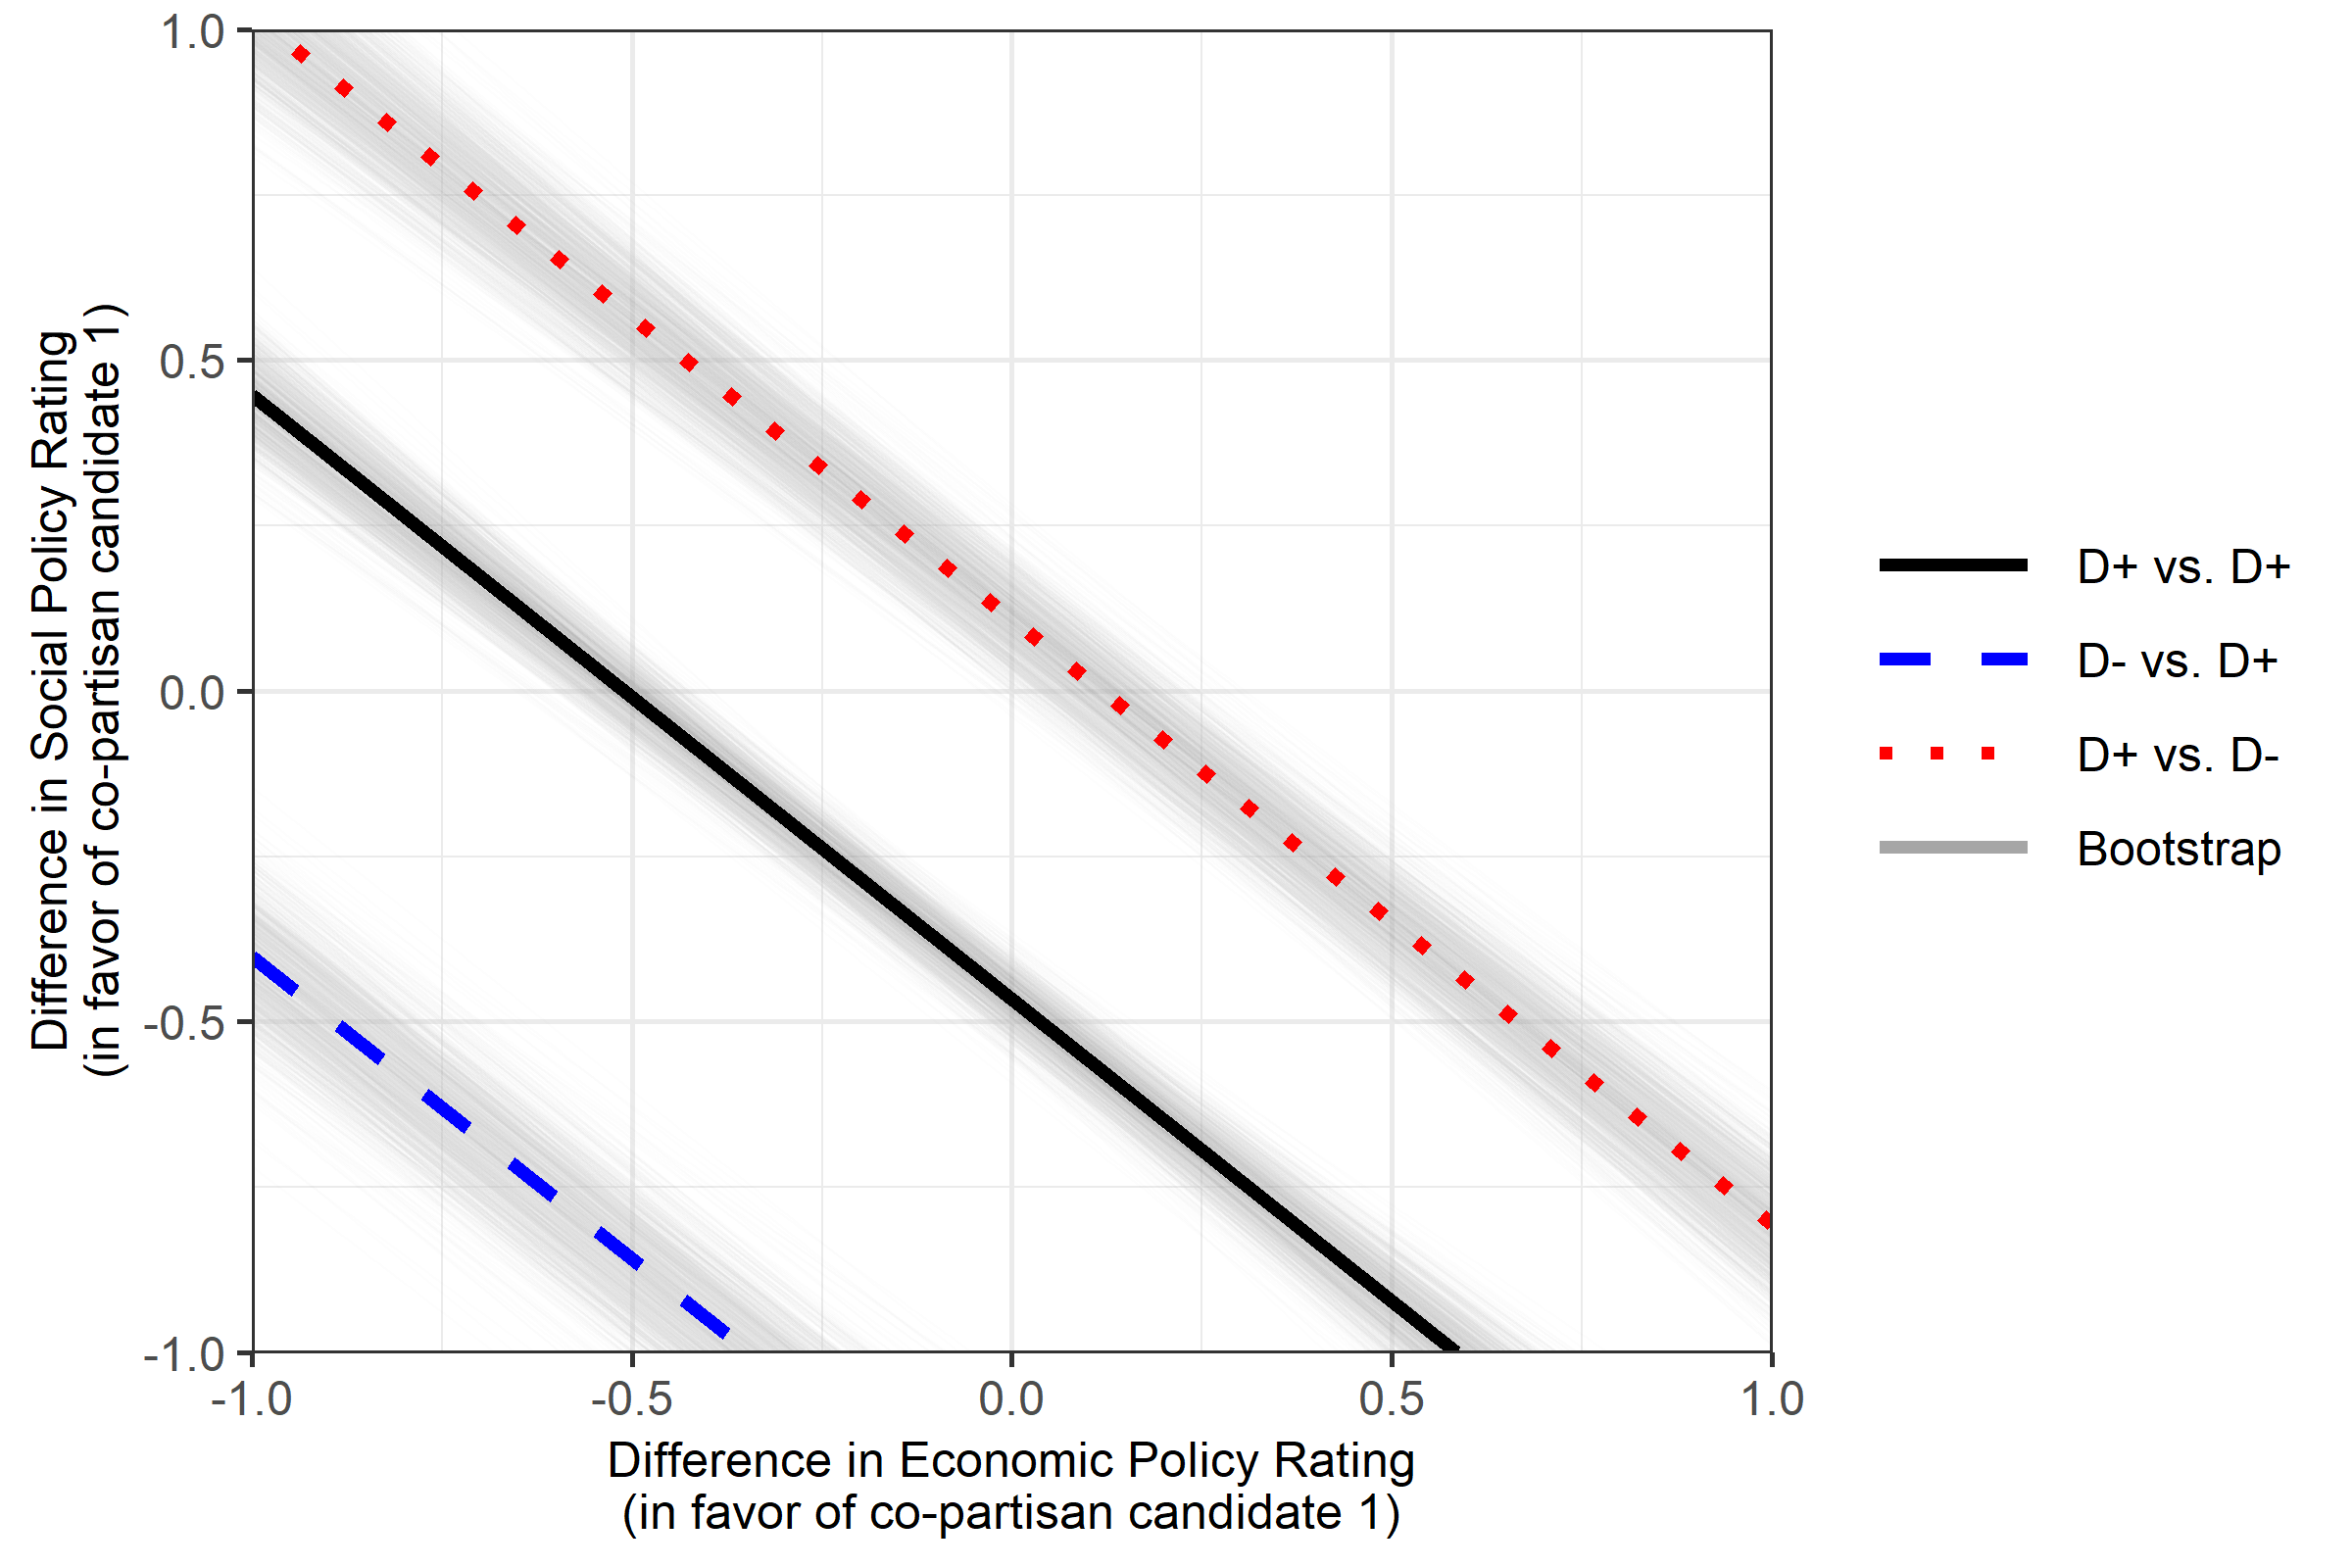
\includegraphics{figures/appendix_structural_isoelects.png}
\caption{Isoelects depicting the combinations of economic and social policies that result in an equal probability of victory for both candidates. Candidate~1 is the respondent's co-partisan, candidate~2 is not; gray bands reflect statistical uncertainty}
\label{fig: mrs_plot}
\end{figure}

The slope of all isoelects is negative ($-\frac{\alpha_1}{\alpha_2}$) with an absolute value smaller than one ($|\frac{\alpha_1}{\alpha_2}|<1$). This implies that voters value a candidate's greater proximity on both economic and social policies but place more weight on the latter.\footnote{A value of 0 on the horizontal and vertical axes refers to scenarios when the respondent rates the two candidates' economic or social platforms equally; positive values correspond to a higher rating of candidate~1's platform.} Meanwhile, voters' value for democracy in terms of economic and social policies corresponds the distance between the $D^+ \text{ vs. } D^+$ and the $D^+ \text{ vs. } D^-$ isoelect along the horizontal and vertical axis, respectively ($\frac{\delta}{\alpha_1}$ and $\frac{\delta}{\alpha_2}$).

The isoelects in Figure \ref{fig: mrs_plot} summarize the impact of partisanship in two ways. First, note that the $D^+ \text{ vs. } D^+$ isoelect is below the point $(0,0)$, reflecting the advantage ($\frac{\alpha_3}{\alpha_2}$) conferred on candidate~1 by his co-partisanship with the respondent. Second, the 50\% bias in the punishment of undemocratic positions that co-partisans benefit from is mirrored in the smaller distance between the $D^+ \text{ vs. } D^+$ and the $D^- \text{ vs. } D^+$ isoelects (compared to the distance between the $D^+ \text{ vs. } D^+$ and the $D^+ \text{ vs. } D^-$ isoelects.)\footnote{This distance is $\frac{\delta}{\alpha_1}(1-\pi)$ and $\frac{\delta}{\alpha_2}(1-\pi)$ along the horizontal and vertical axis, respectively.}

\begin{landscape}
\newgeometry{left=1cm,bottom=2cm,top=2cm,right=-3cm}
\subsubsection{Goodness of fit for the logit model}
In the paper, we justify our use of the logit model by showing that the logit specification is directly implied by our theoretical framework. The figures below provides evidence of goodness of fit by overlaying predictions from logistic regression models onto our non-parametric estimates of candidate support. The figure below presents the same estimates as Section~\ref{sec:fig1} (solid lines) along with predicted values from logit models fit using the same data (dashed lines). The proximity between the solid and dashed lines of the same color indicates the logit model's good fit.

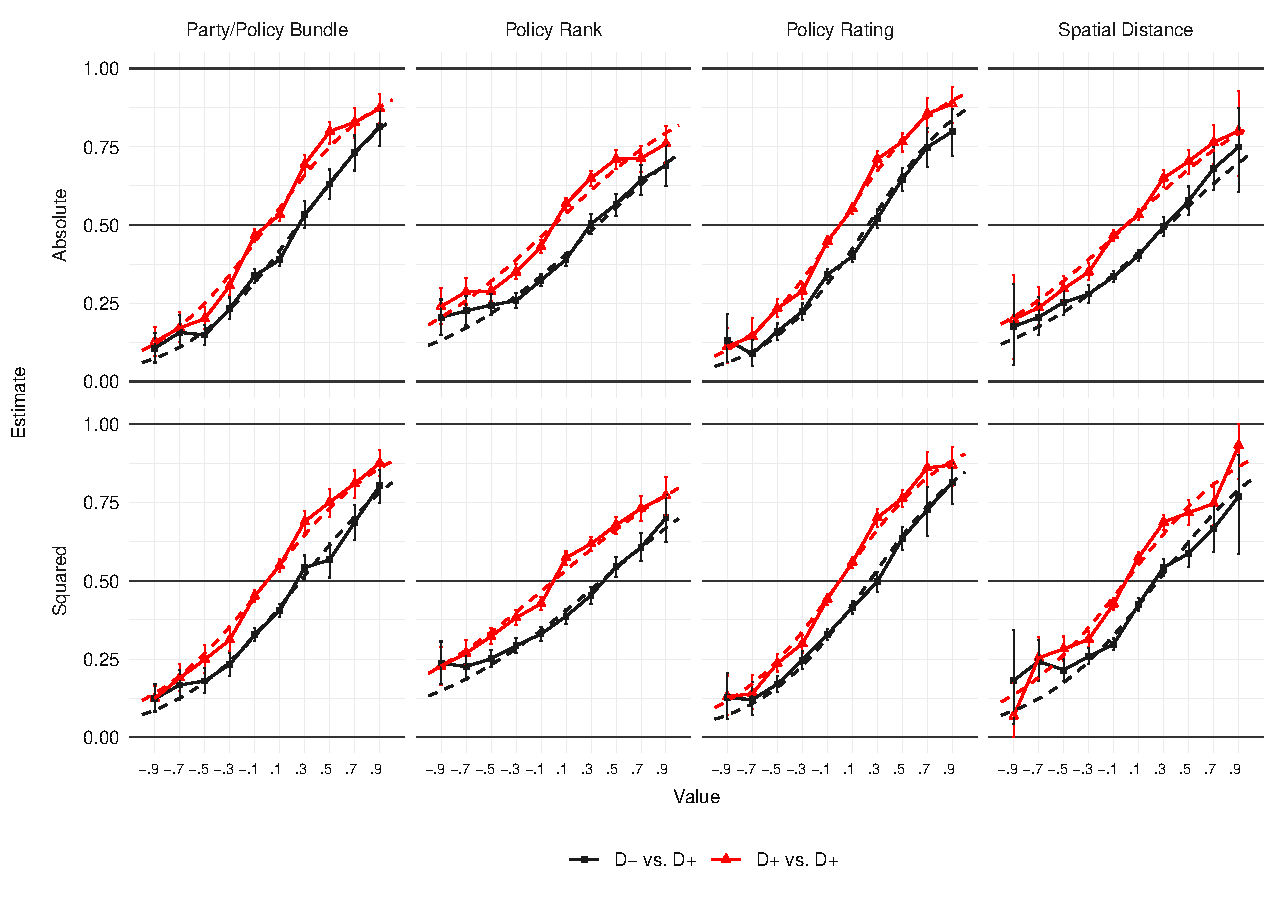
\includegraphics[width=1\textwidth]{figures/appendix_logitFit.pdf}
\restoregeometry
\end{landscape}

\subsubsection{Logistic regression results}

In the main text, Table 2 presents structural estimates of our model's parameters, which were calculated based on logistic regressions. The following tables present results for the underlying logistic regressions.

\begin{table}[ht]
\footnotesize
\centering
\caption{Logistic regression results, standardized}
\label{tab:structureLogit}
\begin{tabular}{lcccccc}
\toprule
& \multicolumn{3}{c}{Core model (column 1)} & \multicolumn{3}{c}{Full model (column 2)} \\
Term & Estimate & SE & CI & Estimate & SE & CI \\
\midrule
\input{figures/appendix_structural_logit_col1-2.txt}
\bottomrule
\end{tabular}
\end{table}

\begin{table}[ht]
\footnotesize
\centering
\caption{Logistic regression results, natural units}
\label{tab:structureLogit}
\begin{tabular}{lcccccc}
\toprule
& \multicolumn{3}{c}{Core model (column 3)} & \multicolumn{3}{c}{Full model (column 4)} \\
Term & Estimate & SE & CI & Estimate & SE & CI \\
\midrule
\input{figures/appendix_structural_logit_col3-4.txt}
\bottomrule
\end{tabular}
\end{table}

\begin{table}[ht]
\footnotesize
\centering
\caption{Logistic regression results with democracy ratings}
\label{tab:structureLogit}
\begin{tabular}{lcccccc}
\toprule
& \multicolumn{3}{c}{Core model (column 5)} & \multicolumn{3}{c}{Full model (column 6)} \\
Term & Estimate & SE & CI & Estimate & SE & CI \\
\midrule
\input{figures/appendix_structural_logit_col5-6.txt}
\bottomrule
\end{tabular}
\end{table}

\clearpage
\newpage

%%%%%%%%%%%%%%%%%%%%%%%%%%%%%%%%%%%%%%%%%
%%%%%%%%%%%%%%%%%%%%%%%%%%%%%%%%%%%%%%%%%

\section{Additional Survey Results}
\setcounter{figure}{0} 
\setcounter{table}{0} 

\onehalfspacing

\subsection{Abstention}

After seeing a profile of two candidates, each respondent was first asked which candidate they preferred and then whether they would vote in an election that pitted the two candidates against each other. The paper focused on the first of these outcomes, the respondents' vote choices. Our analysis therefore uses the outcome variable
$$ Y_i = \mathbbm{1}(\text{prefers candidate 1}) $$
where $\mathbbm{1}()$, the indicator function, returns 1 if the respondent prefers candidate 1 and zero otherwise. We refer to this, for simplicity, as ``voting'' for candidate 1.

To understand how abstention affects undemocratic candidates' fortunes, we defined a new outcome variable
$$ Y_i = \mathbbm{1}(\text{prefers candidate 1 and voted}) $$
which is the outcome variable that is observed in real-world elections. This variable allows us to examine the possibility that undemocratic candidates also suffer due to abstention. When we only count the choices of respondents who also voted---the joint outcome variable that is observed in real elections---the average treatment effect of undemocratic positions rises from 11.7 percentage points to 13.1 percentage points (difference = 1.4 percent, 95\% CI = (0.4, 2.4)). The table below presents the average treatment effect computed using both outcome variables as well as the difference between them. Standard errors and confidence intervals were computed via the block bootstrap.
For a detailed examination of the potential for abstention/turnout to serve as a democratic check, see \citet{GrahamSvolik2019}.
\input{figures/appendix_turnout.txt}

\newpage

\subsection{Do Americans Know What Democracy Is (And Is Not)?}
\label{sec:dem_q}

One potential explanation for our findings – especially those about the limited punishment for candidates who undermine democratic principles -- is that Americans may simply have a poor understanding of what democracy is and what it is not.\footnote{For recent perspectives on how to conceptualize and measure democracy, see \citet{BoixMillerRosato2013}, \citet{Cheibub2010}, and \citet{Coppedge2011}.} In order to evaluate this hypothesis, we included in a survey that preceded the candidate choice experiment by about a week a battery of democratic and undemocratic practices and asked each respondent to evaluate them. Crucially, the undemocratic practices also included items that would later appear as our treatments. To avoid priming our respondents, we intentionally avoided a direct reference to the US context and introduced the battery by the statement: ``Countries around the world differ in how democratic they are. We sampled the following practices from around the world. How democratic do you think each one is?'' This allows us to check whether our respondents understood that the specific practices that would later appear in our treatments were undemocratic, and it does so without alerting respondents to our interest in those specific practices.

In order to verify that respondents also understand what democracy \textit{is}, we also included some perfectly democratic practices, as well as a number of items from the ``essential for democracy'' battery from the World Values Survey. A randomly selected half of our respondents were asked, ``Many things are desirable, but not all of them are essential characteristics of democracy. On a scale from 1 to 10, how essential for democracy is each of the following things?’’ Respondents rated each statement on a 1-10 scale, where 1 means ``not at all democratic'' and 10 means ``completely democratic.'' Before computing the mean ratings, we rescaled the items to range from 0 to 1.

Below, Figures~\ref{fig:dem_treat} and \ref{fig:dem_world}, show that most Americans subscribe to the same conception of democracy that political scientists do. The average rating is below .5 for each of the treatment check items, as well as the ``essential to democracy'' items that describe undemocratic practices (all labelled $D^-$).

For further verification that our respondents are similarly capable of distinguishing democratic, undemocratic, and democratically-neutral practices, we included two batteries of standard questions from the \emph{World Values Survey}. 
Figure~\ref{fig:dem_essential} plots the World Values Survey's ``essential to democracy'' battery and Figure~\ref{fig:dem_sys} plots the World Values Survey's ``political systems'' battery. In both cases, majorities of respondents correctly identified the democratic and undemocratic practices and were about evenly divided over the democratically-neutral practices.

\singlespacing

\begin{figure}[h]
\caption{Ratings of ``around the world'' treatment check statements}
\label{fig:dem_treat}
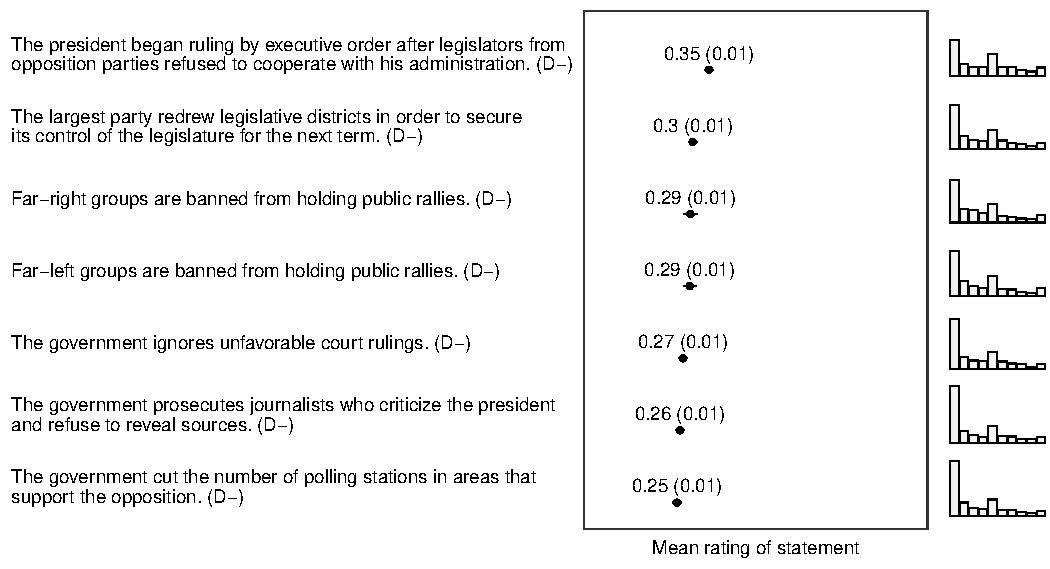
\includegraphics[width=\textwidth]{figures/dem_treat.pdf}
\end{figure}

\begin{figure}[h]
\caption{Ratings of ``around the world'' statements not related to treatment}
\label{fig:dem_world}
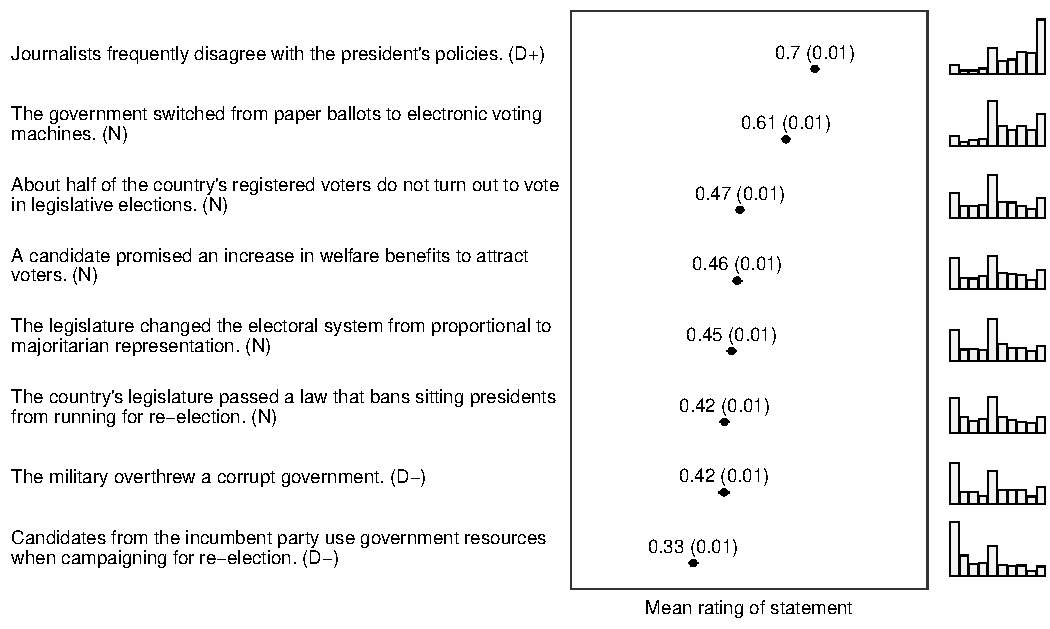
\includegraphics[width=\textwidth]{figures/dem_world.pdf}
\end{figure}

\begin{figure}[h]
\caption{Ratings of World Values Survey ``essential to democracy'' battery}
\label{fig:dem_essential}
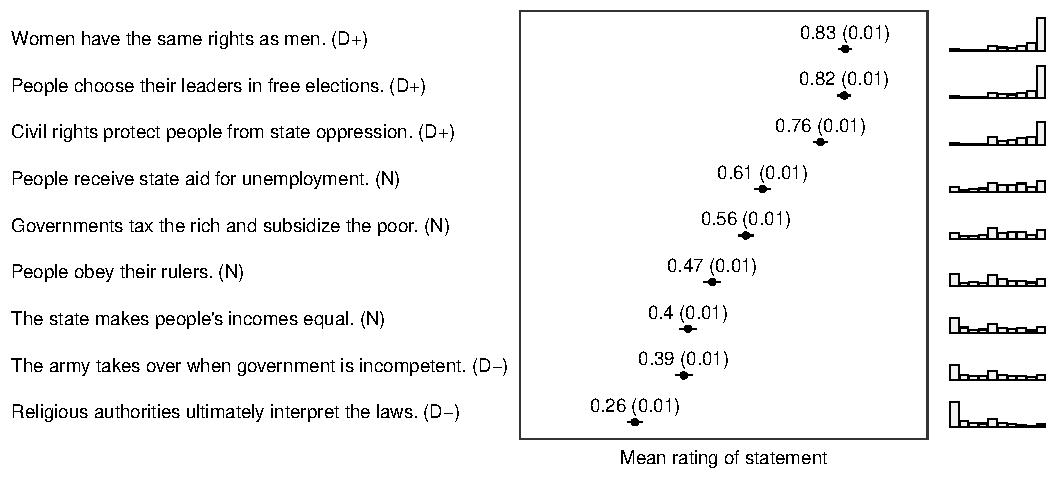
\includegraphics[width=\textwidth]{figures/dem_essential.pdf}
\end{figure}

\begin{figure}[h]
\caption{Ratings of World Values Survey ``political systems'' battery}
\label{fig:dem_sys}
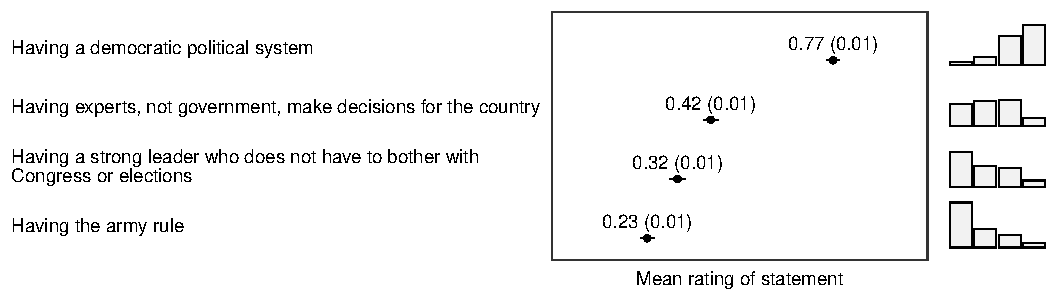
\includegraphics[width=\textwidth]{figures/dem_sys.pdf}
\end{figure}

\begin{figure}[h]
\caption{Ratings of other questions asked of all respondents}
\label{fig:dem_other}
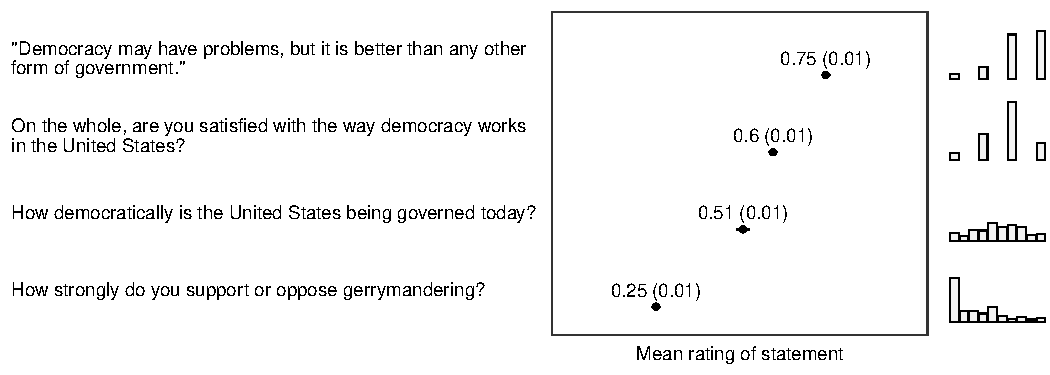
\includegraphics[width=\textwidth]{figures/dem_other.pdf}
\end{figure}

%%%%%%%%%%%%%%

\clearpage

\subsection{Treatment effect heterogeneity by respondent characteristic}

This figure plots treatment effect heterogeneity according to a set of pre-treatment covariates not considered in the body of the paper.

\begin{figure}[h]
\begin{addmargin}{-2em}
\centering
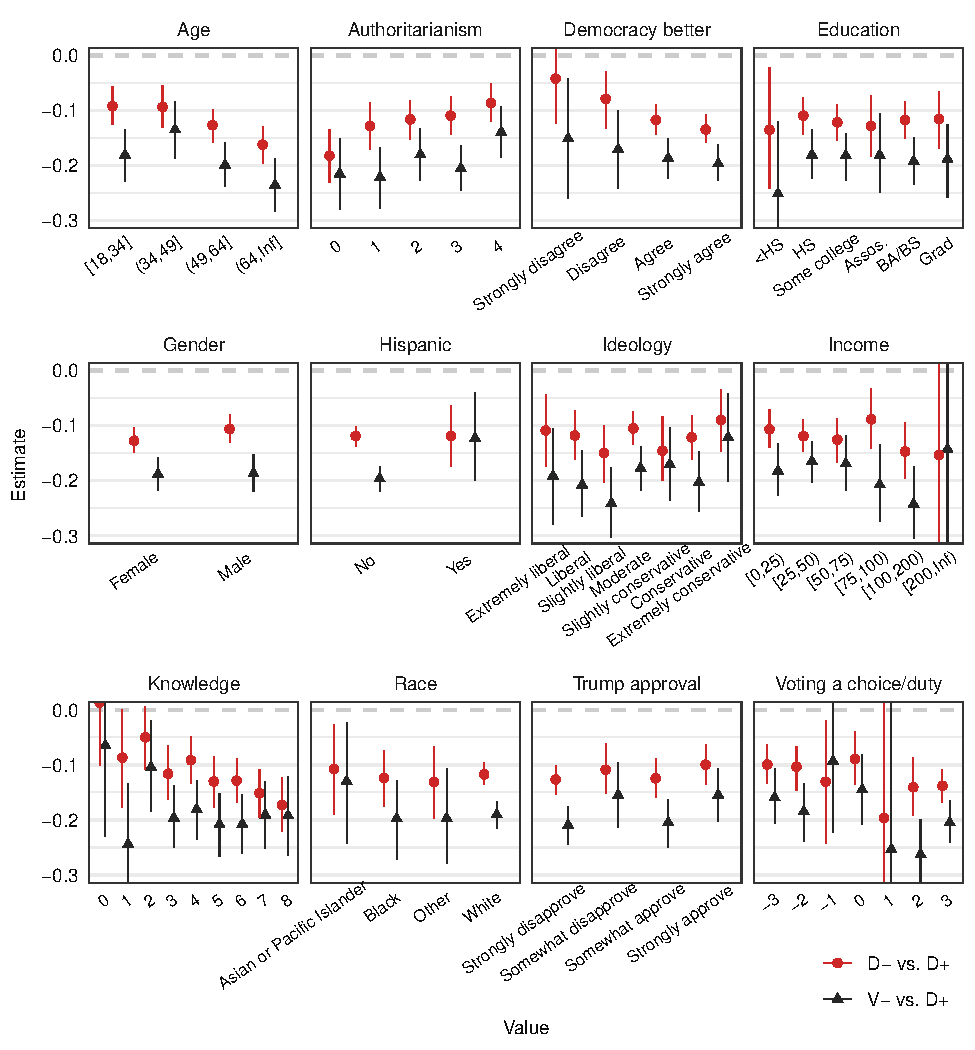
\includegraphics{figures/hetero_trt.pdf}
\end{addmargin}
\end{figure}

\newpage

%%%%%%%%%%%%%%%%%%%%%%%%%%%%%%%%%%%%%%%%%%%%
%%%%%%%%%%%%%%%%%%%%%%%%%%%%%%%%%
%%%%%%%%%%%%%%%%%%%%%%%%%%%%%%%%%

\clearpage
\newpage

\section{The Montana Natural Experiment}
\setcounter{figure}{0} 
\setcounter{table}{0} 

\onehalfspacing

In the paper, we showed that more-Republican precincts were less-punishing of Rep. Greg Gianforte (R-MT)'s assault on a journalist. This section checks the parallel trends assumption, shows that changes in the composition of absentee/polls voters were not associated with the dependent variable, and presents two robustness tests.

\vspace{4mm}

\textit{Parallel trends.} Figure~\ref{fig:mt_parallel} examines the parallel trends assumption \citep[see e.g.][]{AngristPischke2009}. Each square plots the percentage Republican for absentee and election day (``polls") voters, with text indicating the number of voters using each method. Though we only observe one period prior to our diff-in-diff, we observe the behavior of voters in each precinct without error, allowing a precise test of whether each precinct's absentee and polls voters responded similarly to the differences between the candidates in 2014 and 2016. This gives us a precinct-by-precinct proxy for whether absentee and polls voters respond similarly to common shocks.

The shaded squares in Figure~\ref{fig:mt_parallel} flag observations in which the parallel trends assumption appears to be violated. These correspond to the observations we dropped in columns (3) and (4) in the regression table in the paper. Bright pink squares indicate precincts in which the 2014-16 diff-in-diff has an absolute value of more than 10 percentage points. Maroon squares indicate 2014-16 diff-in-diffs with an absolute value of between 5 and 10 percentage points. Grey squares indicate Lake County, for which we do not observe 2014. White squares indicate a 2014-16 diff-in-diff of 5 percentage points or less.

\vspace{4mm}

\textit{Balance on observables.} Another threat to inference in our Montana study is that the composition of absentee and election-day voters in 2016 may have been different than the same composition in 2017. Using the voter file we can create three variables describing the background characteristics of voters in each precinct: age (operationalized by mean birth year), residence within city limits, and percentage of voters voting absentee versus at the polls. Comparing these characteristics with the 2016-17 diff-in-diff provides a check as to whether places with different levels of support for Republicans experienced systematically different changes in the composition of absentee/election-day voters from 2016 to 2017.

To check for an association between observable characteristics and support for Republicans, we plot two versions of each covariate. ``Mean" is simply the mean value of the covariate for all voters in the precinct, pooling across 2016 and 2017. ``D-in-D'' transforms the covariate according to the diff-in-diff formula $(X_{\text{polls,2017}} - X_{\text{absent,2017}}) - (X_{\text{polls,2016}} - X_{\text{absent,2016}})$. Figure~\ref{fig:mt_covar_pctR} plots these measures against the percentage of voters in the precinct supporting Republicans in 2016 (i.e., the interaction term in the interacted diff-in-diff). Figure~\ref{fig:mt_covar_dId} plots the same measures against the 2016-17 percent Republican diff-in-diff (i.e., the dependent variable). The plots suggest that there is no major systematic relationship between baseline voter characteristics and the key variables.

\vspace{4mm}

\textit{Dropping controls.} Table~\ref{tab:mt_reg_noctrl} verifies that our main result is robust to the exclusion of control variables. Although we can no longer detect the overall average effect of the attack, we still detect a large, statistically significant difference between more- and less-Republican precincts.

\vspace{4mm}

\textit{Placebo test.} As a check that our results are not spurious, Tables~\ref{tab:mt_placebo_ctrl} and \ref{tab:mt_placebo_noctrl} present regression results from placebo tests using the difference between 2014 and 2016 instead of 2016 and 2017. We never detect a negative main effect (2016 $\times$ electDay) or a positive interaction effect (2016 $\times$ Elect Day $\times$ \% R 2014), suggesting that the key results in the paper were not spurious. We do detect some placebo effects with the wrong sign in the full sample, but not for the restricted sample of counties that met our parallel trends criteria.

\singlespacing

\newgeometry{left=2cm,bottom=2cm,top=1cm,right=-3cm}
\begin{landscape}
\subsection{Parallel trends}
\begin{figure}[h]
\caption{Montana parallel trends by precinct\label{fig:mt_parallel}}
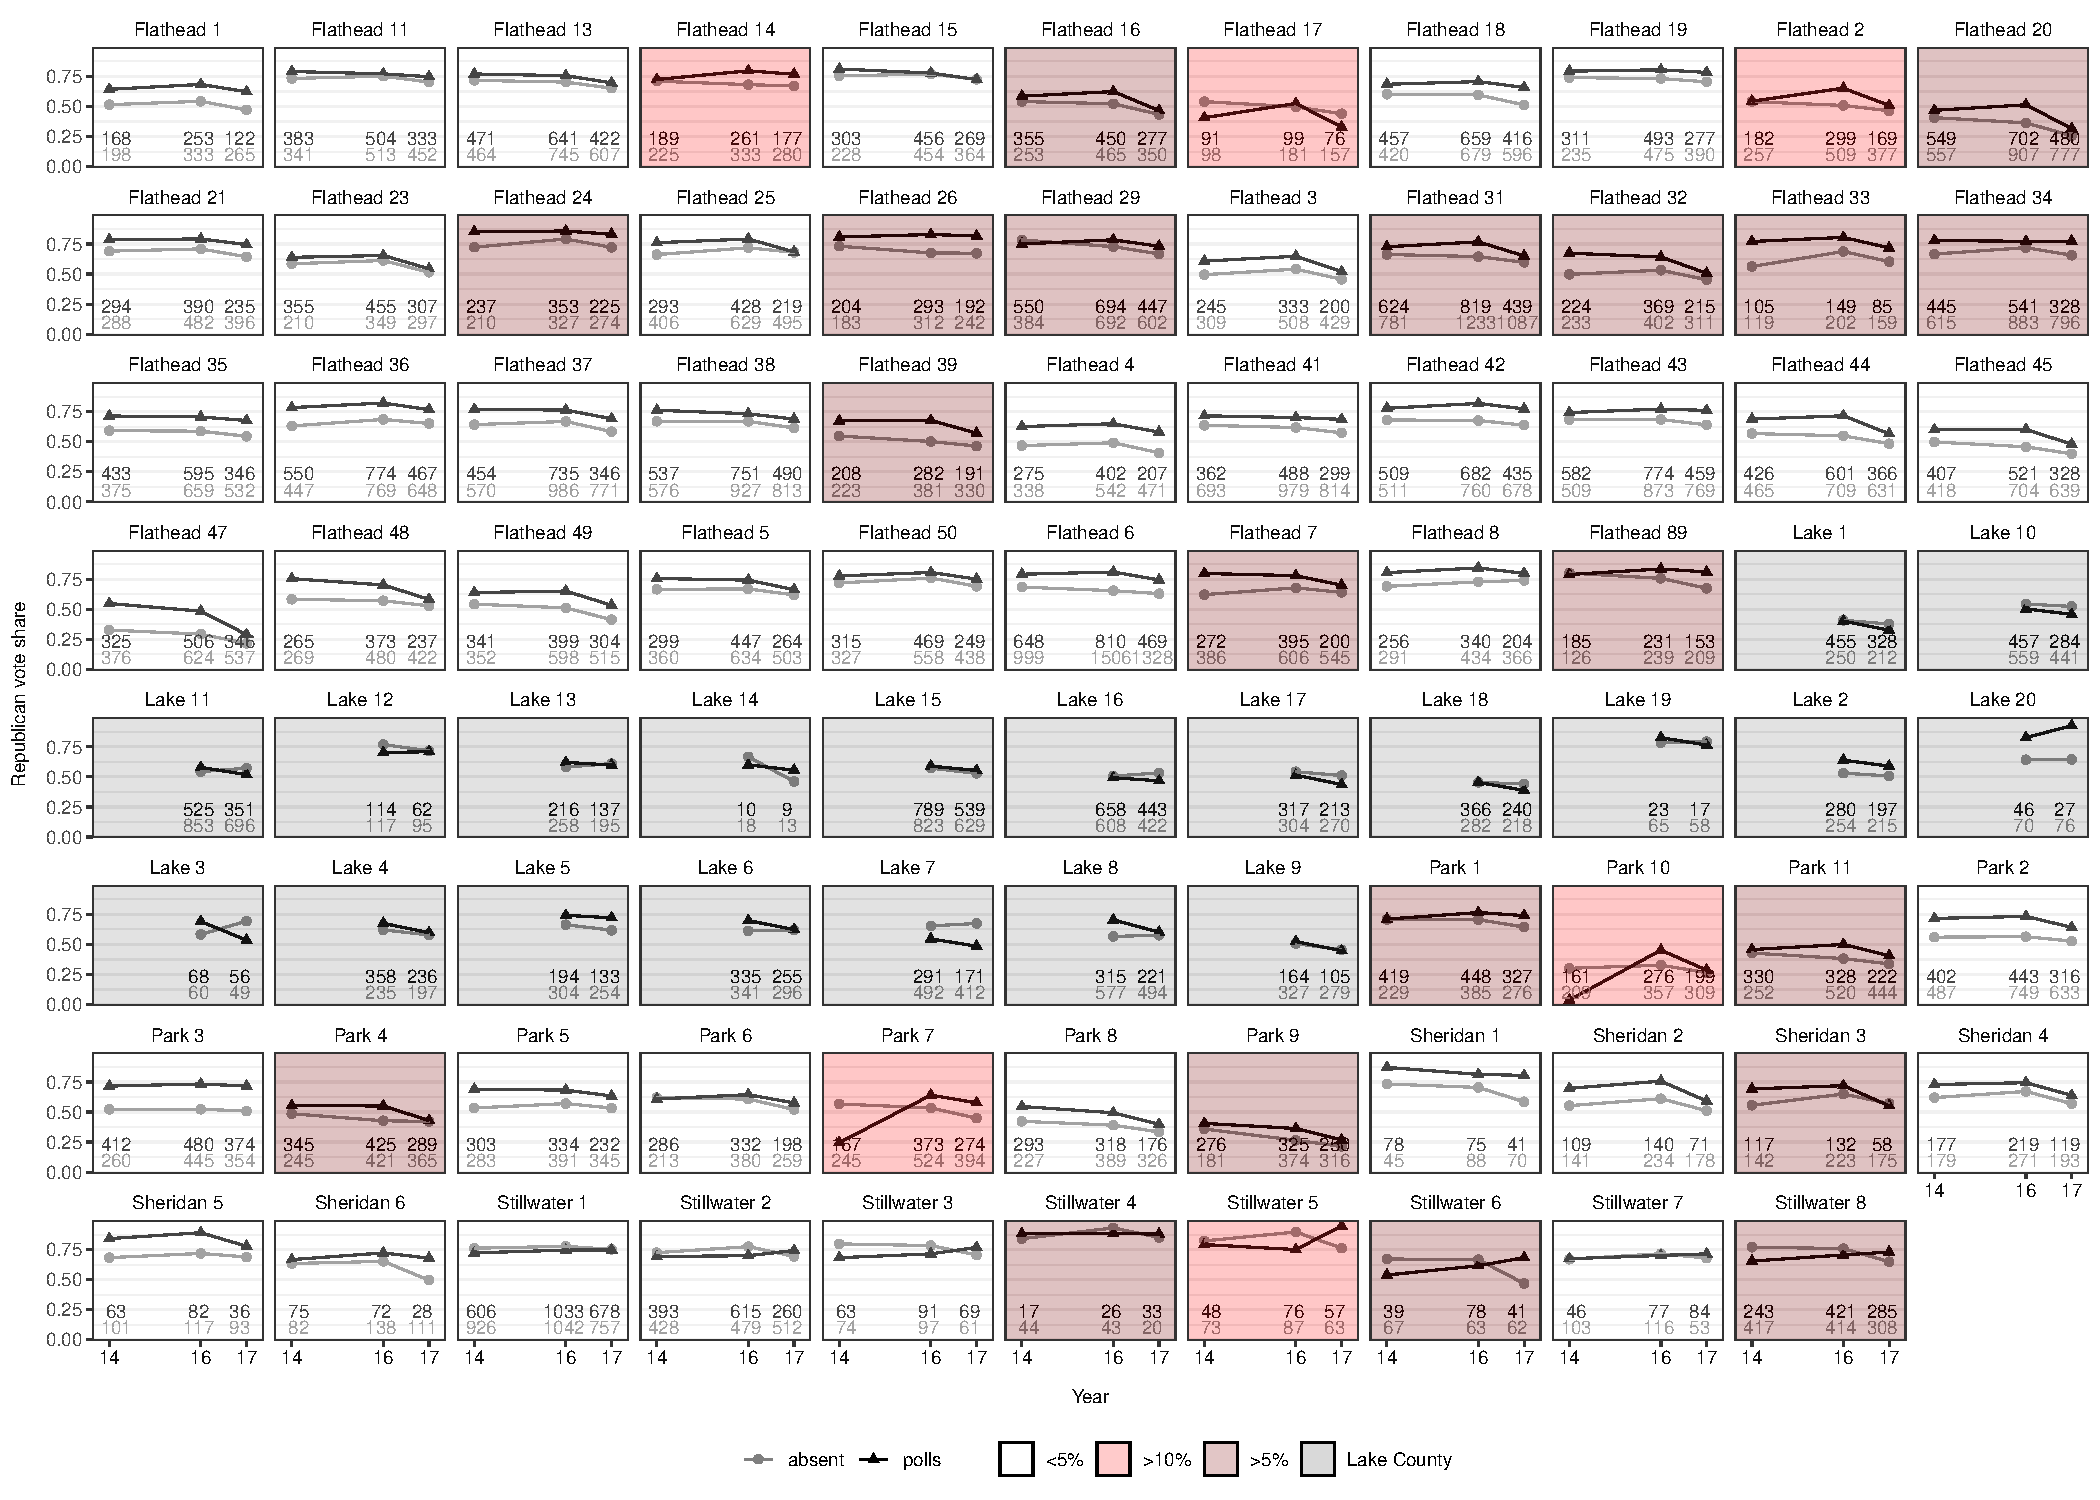
\includegraphics[width=\textwidth]{figures/mt_parallel.pdf}
\end{figure}
\end{landscape}
\restoregeometry

\clearpage

\newgeometry{left=2cm,bottom=-3cm,top=1cm,right=2cm}
\subsection{Balance on observable characteristics}
\vspace{-4mm}
\begin{figure}[h]

\caption{Montana covariate balance vs. dependent variable\label{fig:mt_covar_dId}}
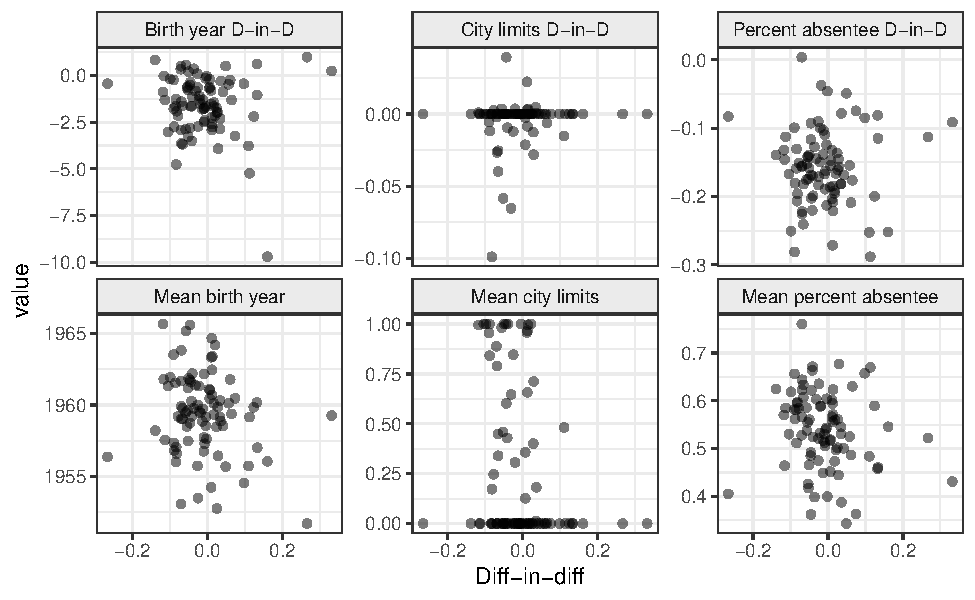
\includegraphics[width=\textwidth]{figures/mt_covar_dId.pdf}

\caption{Montana covariate balance vs. percent Republican support\label{fig:mt_covar_pctR}}
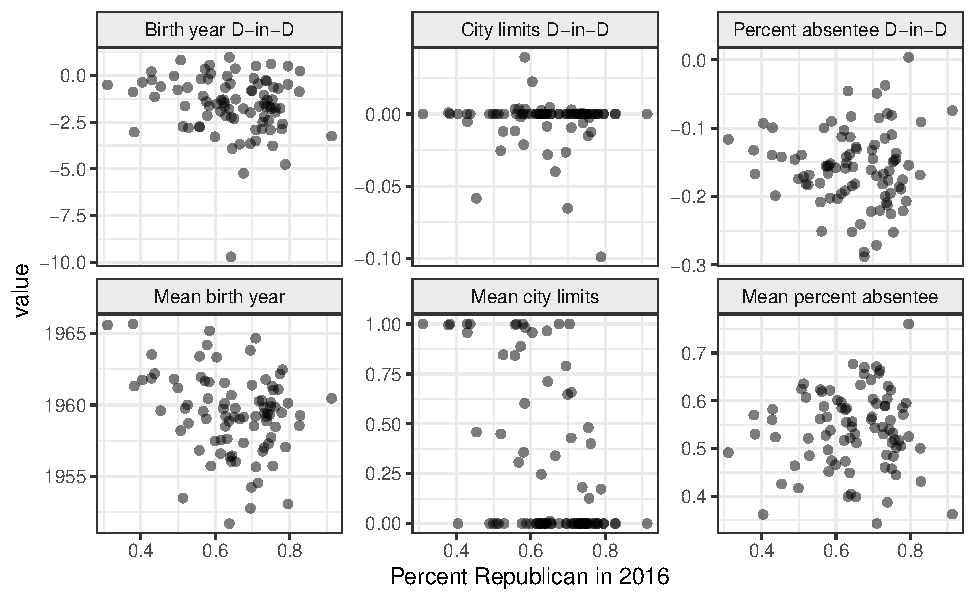
\includegraphics[width=\textwidth]{figures/mt_covar_pctR16.pdf}


\end{figure}
\restoregeometry

\clearpage
\newgeometry{left = 2cm, bottom = 1.1cm, top = 2cm, right = 2cm}
\subsection{Full regression table}

\input{figures/mt_regTab_ctrl.txt}
\vspace{-1cm}

\clearpage
\newpage

\subsection{No-controls regression}

\input{figures/mt_regTab_noctrl.txt}

\clearpage
\newpage

\subsection{Placebo tests}

\input{figures/mt_placeboTab_ctrl.txt}

\clearpage

\input{figures/mt_placeboTab_noctrl.txt}

\restoregeometry
\newpage

\subsection{Relationship between geographic and individual characteristics}

\onehalfspacing

Our Montana study uses the percentage of Republicans in a precinct as an indicator of precinct extremism. To examine the relationship between Republican vote share and individual-level indicators of partisanship and ideology, Figure~\ref{fig:mt_geogVsIndiv} merges data from the 2016 Cooperative Congressional Election Survey (CCES) and county-level returns from the 2016 presidential election. In each panel, the X-axis is the county-level presidential Republican vote share and the Y-axis is one measure of CCES respondents' partisan and ideological leanings. All measures were standardized to have a mean of zero and the standard deviation of one.

Each panel shows that respondents in counties that vote more Republican tend to be more conservative, even within political party. The solid line is a loess line and the dotted line is an OLS regression. The table below displays the slope coefficient for each OLS line with each measure rescaled to [0, 1] for comparability. 

Both the figure and the table show that even within party, more Republican counties have more conservative and Republican voters. The first panel shows that Democrats, independents, and Republicans place themselves as more conservative on a five-point liberal-conservative scale. The second panel shows that Democrats are weaker partisans and Republicans are stronger partisans in areas that vote more Republican. Pure (non-leaning) independents are excluded because they only take one value on the seven-point party identification scale. The third panel shows that in more Republican counties, each partisan group is more disapproving of President Obama. The fourth panel uses item response theory (IRT)-based ideal points computed for \citet{GrahamOrr2020}. Each partisan group is more conservative in counties that vote more Republican. The fifth panel shows the same pattern using the additive score ideal points from the appendix to \citet{GrahamOrr2020}.

\singlespacing

\begin{landscape}
\bgroup
\small
\input{figures/mt_geogVsIndiv.txt}
\egroup
\end{landscape}


\begin{landscape}
\begin{figure}

\caption{Relationship between presidential vote share and within-party conservatism\label{fig:mt_geogVsIndiv}}
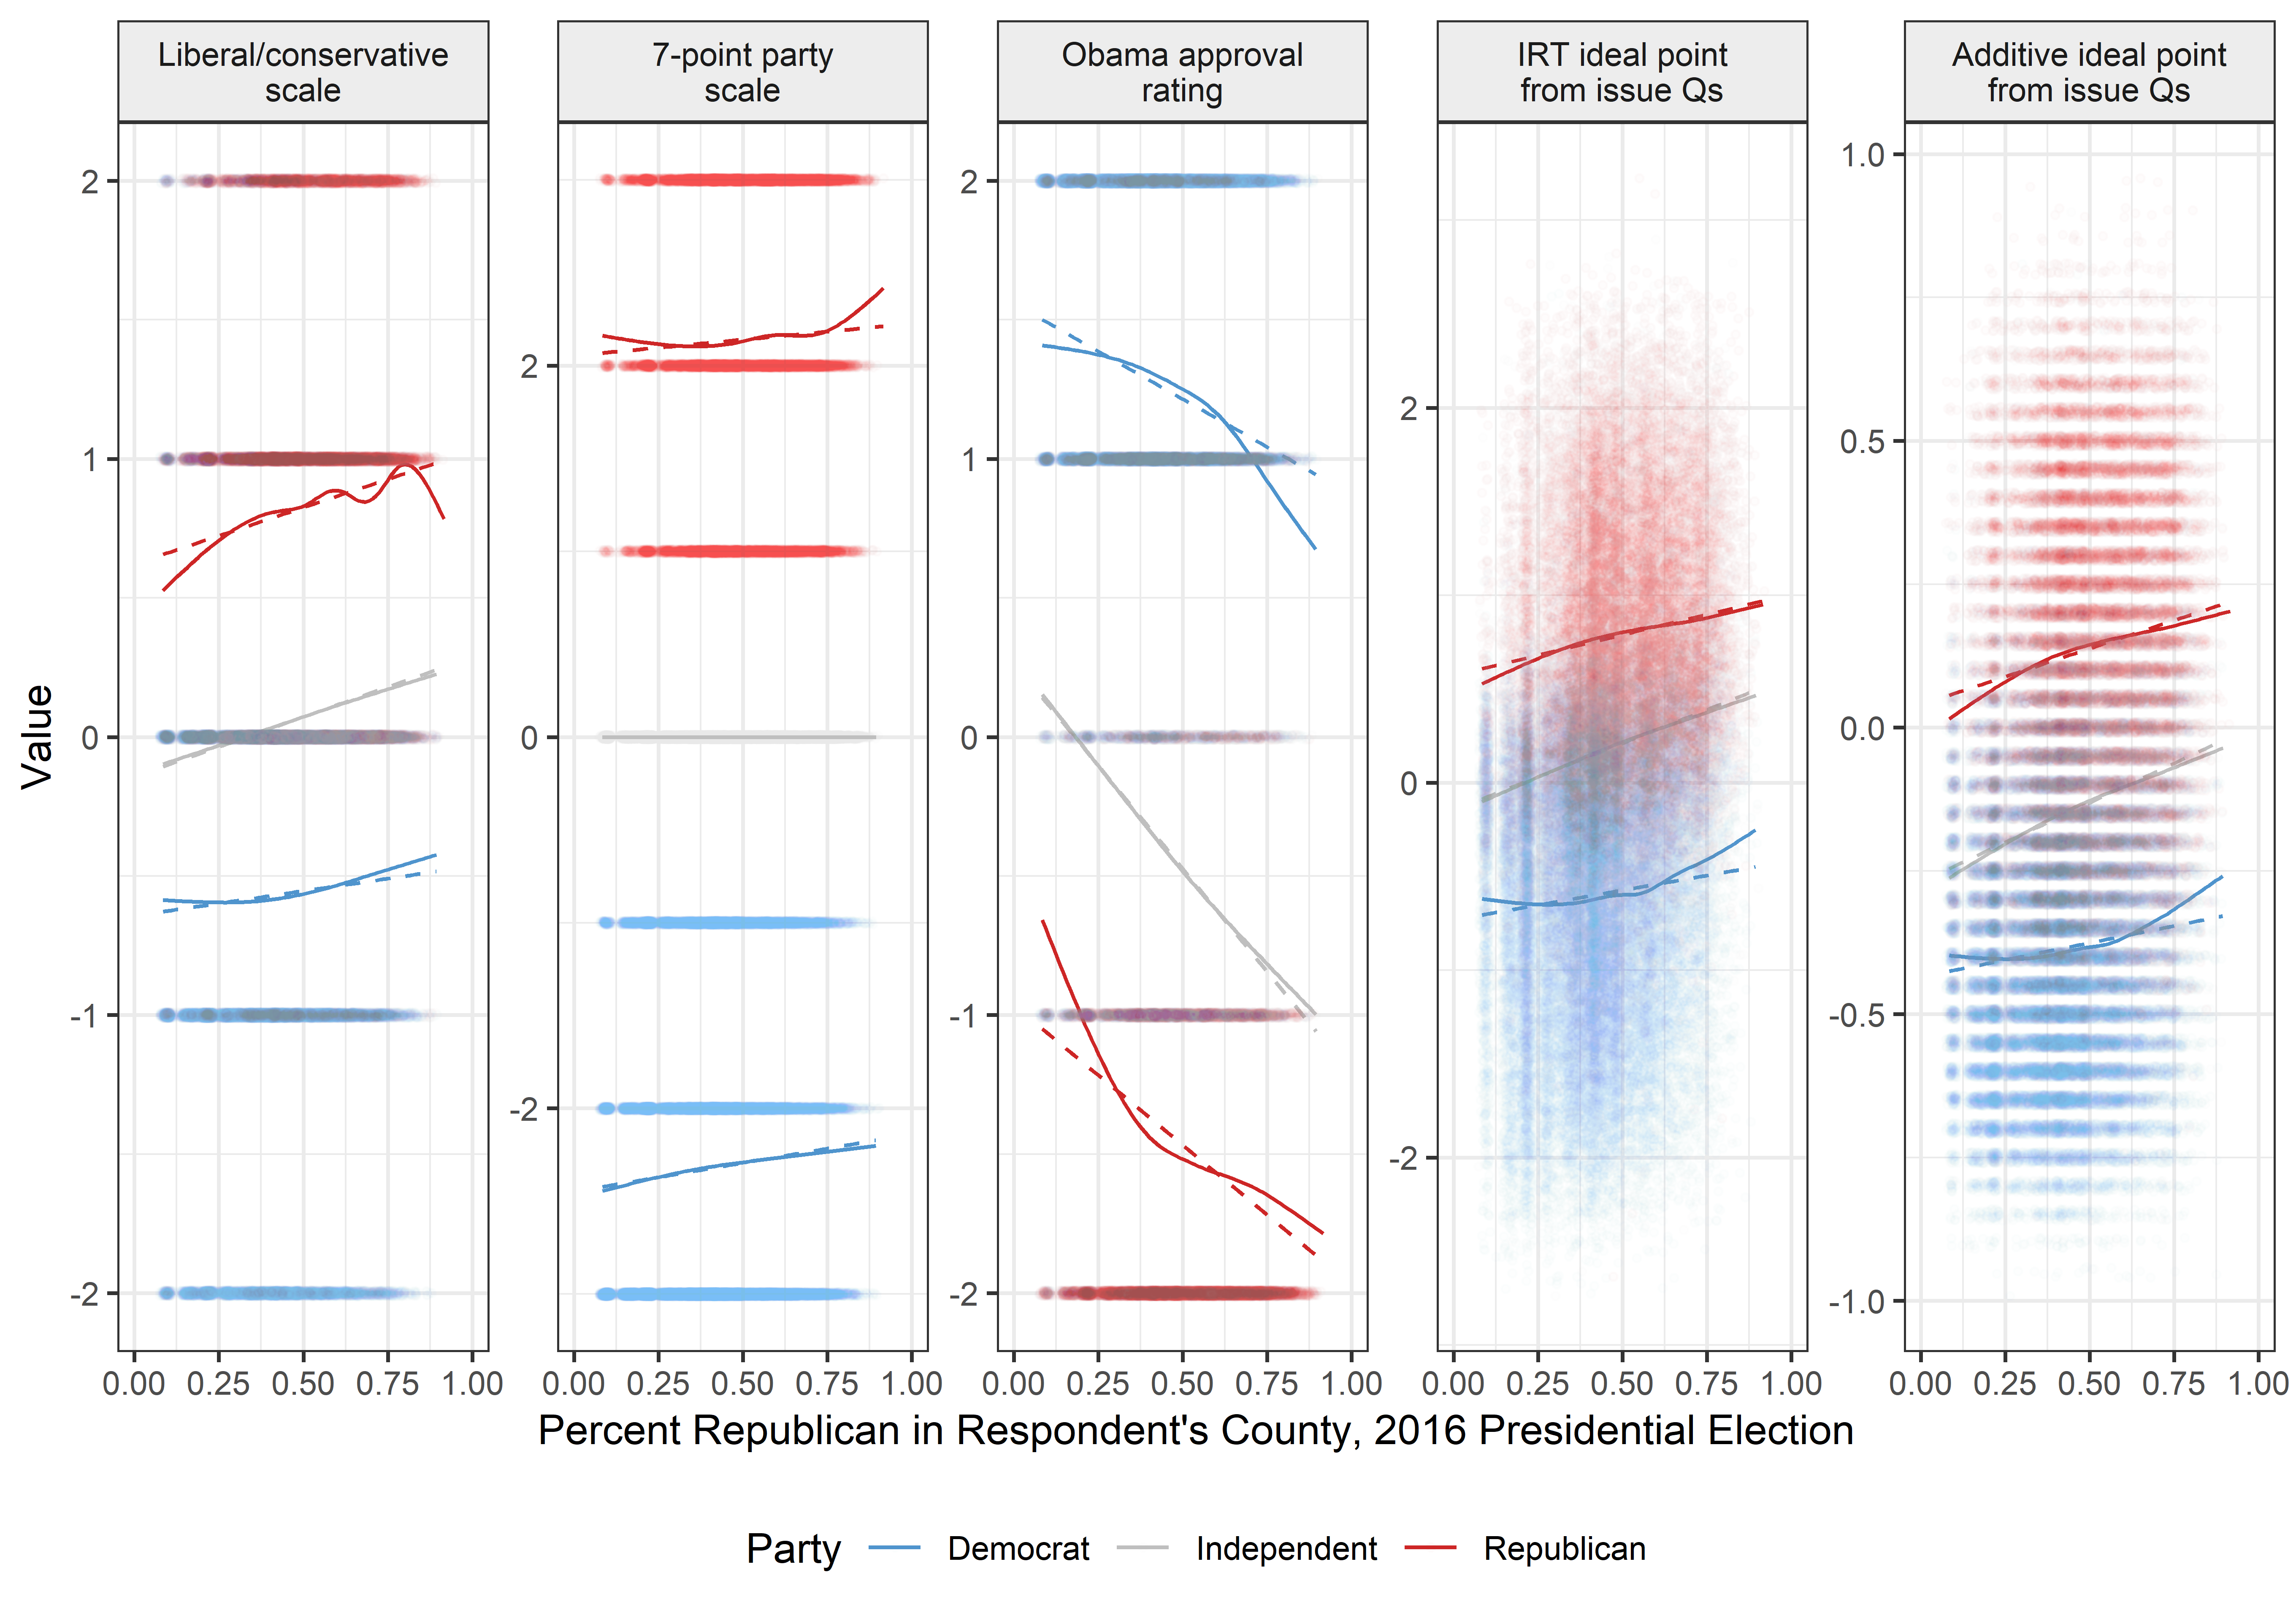
\includegraphics{figures/mt_geogVsIndiv.png}

\end{figure}
\end{landscape}

%%%%%%%%%%%%%%%%%%%%%%%%%%%%%%%%%%%%%%%%%%%%%
%%%%%%%%%%%%%%%%%%%%%%%%%%%%%%%%%%%%%%%%%%%%%
%%%%%%%%%%%%%%%%%%%%%%%%%%%%%%%%%%%%%%%%%%%%%

\clearpage
\newpage


\section{Full Survey Text}

\onehalfspacing

The following pages contain screenshots for each page of the questionnaire, in the order they appeared in one run through the survey. For branching questions (e.g., the ANES 7-point party identification questions), only one possible branch appears.

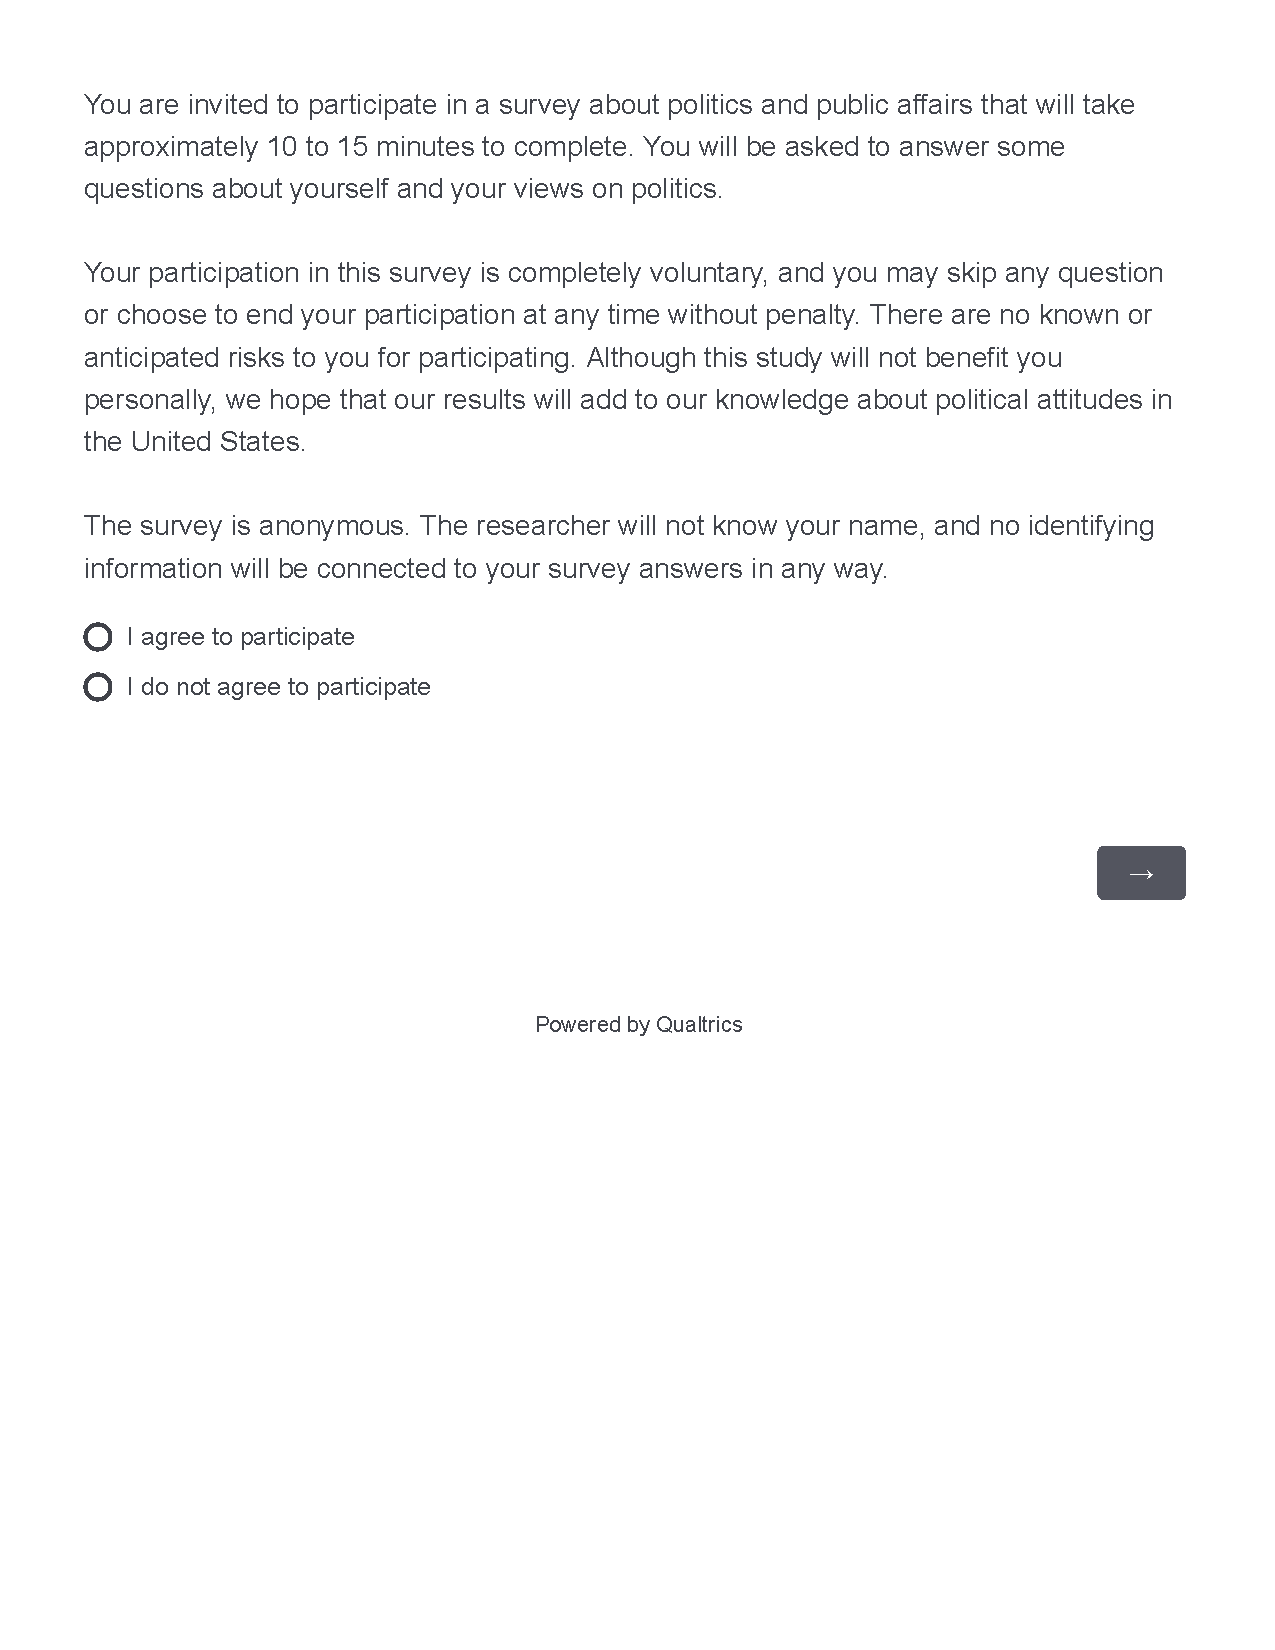
\includepdf[page=-]{figures/screenByScreen_wave1}
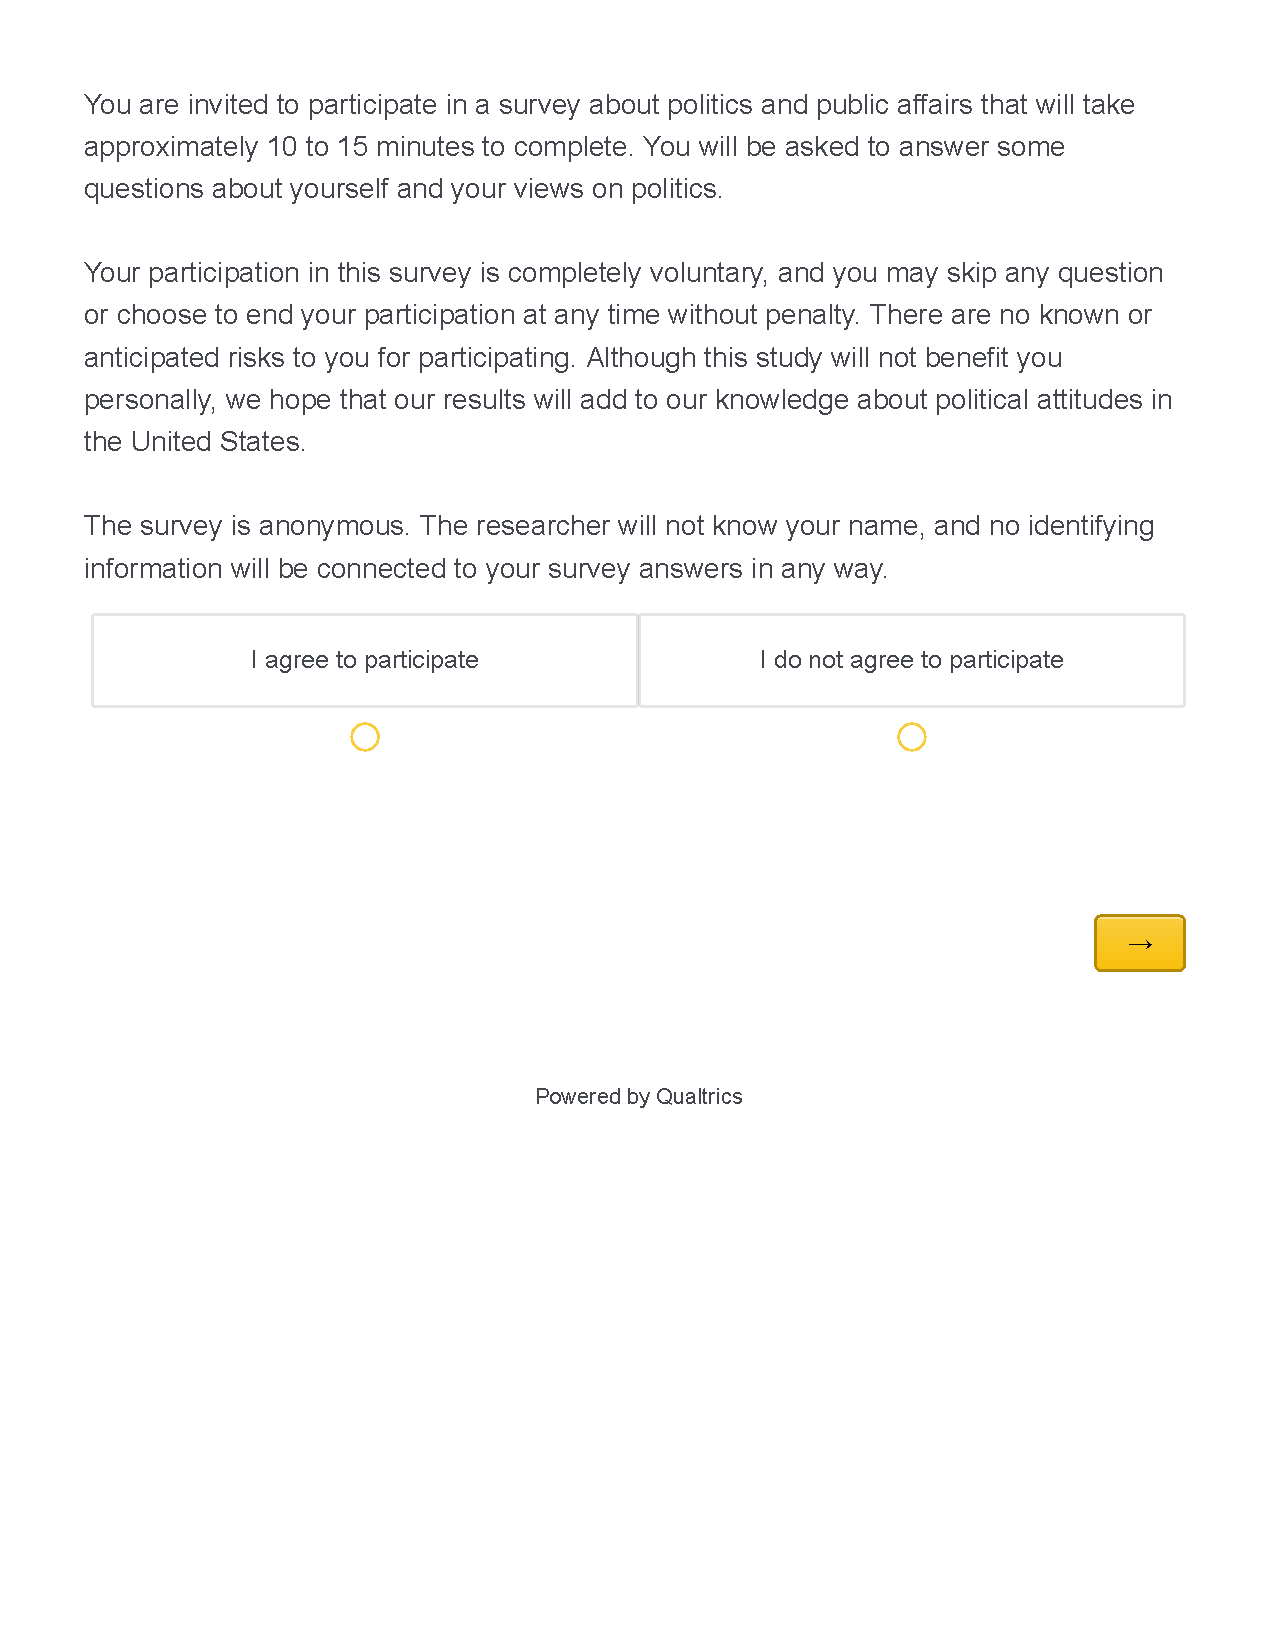
\includepdf[page=-]{figures/screenByScreen_wave2}

\clearpage
\newpage

\singlespacing

\bibliographystyle{myapsr}
\bibliography{combined_bib}

\end{document}

